%%%%%%%%%%%%%%%%%%%%%%%%%%%%%%%%%%%%%%%%%%%%%%%%%%%%%%%%%%%%%%%%%%%%
%% I, the copyright holder of this work, release this work into the
%% public domain. This applies worldwide. In some countries this may
%% not be legally possible; if so: I grant anyone the right to use
%% this work for any purpose, without any conditions, unless such
%% conditions are required by law.
%%%%%%%%%%%%%%%%%%%%%%%%%%%%%%%%%%%%%%%%%%%%%%%%%%%%%%%%%%%%%%%%%%%%

\documentclass[
  digital, %% This option enables the default options for the
           %% digital version of a document. Replace with `printed`
           %% to enable the default options for the printed version
           %% of a document.
  table,   %% Causes the coloring of tables. Replace with `notable`
           %% to restore plain tables.
  lof,     %% Prints the List of Figures. Replace with `nolof` to
           %% hide the List of Figures.
  lot,     %% Prints the List of Tables. Replace with `nolot` to
           %% hide the List of Tables.
  %% More options are listed in the user guide at
  %% <http://mirrors.ctan.org/macros/latex/contrib/fithesis/guide/mu/fi.pdf>.
]{fithesis3}
%% The following section sets up the locales used in the thesis.
\usepackage[resetfonts]{cmap} %% We need to load the T2A font encoding
\usepackage[T1,T2A]{fontenc}  %% to use the Cyrillic fonts with Russian texts.
\usepackage[
  main=english, %% By using `czech` or `slovak` as the main locale
                %% instead of `english`, you can typeset the thesis
                %% in either Czech or Slovak, respectively.
  %%german, russian, czech, slovak %% The additional keys allow
]{babel}        %% foreign texts to be typeset as follows:
%%
%%   \begin{otherlanguage}{german}  ... \end{otherlanguage}
%%   \begin{otherlanguage}{russian} ... \end{otherlanguage}
%%   \begin{otherlanguage}{czech}   ... \end{otherlanguage}
%%   \begin{otherlanguage}{slovak}  ... \end{otherlanguage}
%%
%% For non-Latin scripts, it may be necessary to load additional
%% fonts:
\usepackage{paratype}
\def\textrussian#1{{\usefont{T2A}{PTSerif-TLF}{m}{rm}#1}}
%%
%% The following section sets up the metadata of the thesis.
\thesissetup{
    date          = \the\year/\the\month/\the\day,
    university    = mu,
    faculty       = fi,
    type          = mgr,
    author        = Bc. Pavol Loffay,
    gender        = m,
    advisor       = RNDr. Adam Rambousek\, Ph.D.,
    title         = {Alert Prediction in Metric Data Based on Time Series Analysis},
    TeXtitle      = {Alert Prediction in Metric Data Based on Time Series Analysis},
    keywords      = {Time Series, Hawkular, Alert Prediction, Exponential Smoothing},
    TeXkeywords   = {Time Series, Hawkular, Alert Prediction, Exponential Smoothing},
}
\thesislong{abstract}{
  The aim of the master's thesis is to develop a module for an open source monitoring
  and management platform Hawkular. This module is responsible for predicting
  alerts based on time series and providing data for predictive charts in Hawkular user interface.
}
\thesislong{thanks}{
  I would like to thank my supervisor RNDr. Adam Rambousek, Ph.D., Mgr. Jiri Kremser,
  family and the people from Hawkular team. Next, my thanks goes to Ing. Daniel Němec, Ph.D.
  for consulting theory behind time series analysis.

  Last but not least, I would like to thank to company Red Hat that provided me
  the great opportunity to work on this project.
}
%% The following section sets up the bibliography.
\usepackage{csquotes}
%\usepackage[              %% When typesetting the bibliography, the
%  backend=biber,          %% `numeric` style will be used for the
%  style=numeric,          %% entries and the `numeric-comp` style
%  citestyle=numeric-comp, %% for the references to the entries. The
%  sorting=none,           %% entries will be sorted in cite order.
%  sortlocale=auto         %% For more unformation about the available
%]{biblatex}               %% `style`s and `citestyles`, see:
%% <http://mirrors.ctan.org/macros/latex/contrib/biblatex/doc/biblatex.pdf>.
%\addbibresource{bibliography.bib} %% The bibliograpic database within
                          %% the file `example.bib` will be used.
\usepackage{makeidx}      %% The `makeidx` package contains
\makeindex                %% helper commands for index typesetting.
%% These additional packages are used within the document:
\usepackage{paralist}
\usepackage{amsmath}
\usepackage{amsthm}
\usepackage{amsfonts}
\usepackage{url}
\usepackage{menukeys}
\usepackage{multicol}

%My papckages
%\DeclareUrlCommand\url{\def\UrlLeft{<}\def\UrlRight{>} \urlstyle{tt}}
\usepackage{graphicx}
\usepackage{float}
\usepackage{commath} % abs
\usepackage{listings}
\usepackage{algorithm} %algorithmix
\usepackage[noend]{algpseudocode}
\lstset{language=java}
\usepackage{pgf-pie}
\usepackage{multirow}
\usepackage{tabularx}

\usepackage{xparse}
\NewDocumentCommand{\INTERVALINNARDS}{ m m }{
    #1 {,} #2
}
\NewDocumentCommand{\interval}{ s m >{\SplitArgument{1}{,}}m m o }{
    \IfBooleanTF{#1}{
        \left#2 \INTERVALINNARDS #3 \right#4
    }{
        \IfValueTF{#5}{
            #5{#2} \INTERVALINNARDS #3 #5{#4}
        }{
            #2 \INTERVALINNARDS #3 #4
        }
    }
}

\hyphenation{data-bases}
\hyphenation{gar-bage}
\hyphenation{re-using}

\begin{document}
% Author: Pavol Loffay
% Project: Master thesis - Hawkular alert prediction
% Date 20.2.2015

% Cross-Referencing Conventions:
% chap: chapter
% sec: section
%
% appen: everything from appendix, e.g. appen:img:foo
%
% eq: equation
% img: image
% tab: table
% alg: algorithms
% item: item in itemize
%
% example \label{img:foo-foo}
%%%%%%%%%%%%%%%%%%%%%%%%%%%%%%%%%%%%%%%%%%%%%%%%%%%%%%%%%%%%%%%%%%%
\chapter{Introduction} \label{chap:introduction}
When driving successful business on the internet, it is important to assure application`s health and reliability. One
can achieve that by monitoring subjected resources and setting up clever alerting system.

These features are offered by many monitoring systems, however being predictive in this area can even prevent
undesirable states and most importantly gives administrators more time to react to such \\events. For instance it
can decrease downtime of an application or ability to load balance workload in advance by horizontal scaling of
targeted services.

Alerting systems are sophisticated and can be composed by many conditions. This work focuses on predicting future
metric values \\which are then sent as input for evaluation to alerting system.

The work starts with time series theory by describing various approaches for time series modelling and forecasting.
The chapter describes models which are used within the work, could be used or explains why the decision was made to
use other models.

Following chapter demonstrates models from previous chapter on real time series. It visually shows predictive
capabilities of targeted models and compares produced statistical quantities.

The third chapter briefly describes existing monitoring and management solutions which are to some extend
Hawkular competitors. Java libraries for time series forecasting are also mentioned there.

The fourth chapter describes implementation part of the thesis. It starts with core artifacts for time series
forecasting and continues to building web application and integration into Hawkular.

The last chapter is dedicated to the evaluation of the forecasting accuracy of the implemented solution.
Models from \texttt{forecast} package from language R were chosen as a referential implementation.

    %%%%%%%%
    \section{Hawkular} \label{sec:hawkular}
    The implementation part of the master's thesis is developed as a part of an open source project
    Hawkular\footnote{Available at \url{http://www.hawkular.org}}, therefore, the application architecture and used
    technologies had to fit into the overall project design.

    Hawkular is middleware monitoring and management platform developed by company Red Hat and independent community
    of contributors. It is a successor of very successful RHQ\footnote{Available at
    \url{https://rhq-project.github.io/rhq/}.} project, also known as JBoss Operations Network (JON). By monitoring,
    it is meant that there are agents for diverse applications which push data to the server. These agents can also
    execute application specific actions.

    The monolithic architecture of the RHQ project was due to its size hard to maintain and lacking robust REST API
    lead to fresh development of new application. Hawkular, in contrast, consists of several loosely coupled or even
    independent applications. These independent components are much easier to maintain and what is more important they
    communicate over REST API.

    This architecture of microservices and chosen protocol allow simple development of agents which can be
    written in any programming language. In RHQ only Java agent were available.

    Hawkular as a product itself is customized
    Wildfly\footnote{An open source project of JBoss Enterprise Application Platform.} application server with all
    components deployed in it.

    List of Hawkular main components:
    \begin{itemize}
        \item Console\,--\,user web interface.
        \item Accounts\,--\,authorization subsystem based on Keycloak\footnote{An open
            source single sing-on and identity management for RESTful web services.}.
        \item Inventory\,--\,graph based registry of all entities in Hawkular.
        \item Metrics\,--\,time series metrics engine based on Cassandra\footnote{An open
            source distributed database management system. Hybrid between key-value and
        column-oriented database.}.
        \item Alerts\,--\,alerting subsystem based on JBoss Drools.
    \end{itemize}

    Some of the modules also use Java messaging system (JMS) for inter-component communication.

    Modules are packaged as standard Java web archives (WAR), or enterprise archives (EAR) and deployed into Wildfly.
    Build and package management is performed by Maven and Gulp for user interface modules.

    %%%%%%%%
    \section{Data Mining Goals} \label{sec:goals}
    The goal of this thesis is to develop a module for Hawkular which will provide forecasts for any time series
    metrics collected by agent.

    Module should learn from new incoming metric data and immediately send predicted values for future timestamps to
    alerting subsystem. Based on this values an alert can be triggered. This implies that forecasting engine should
    work on continuous flow of data. Forecast should be also available for user interface in predictive charts.

    One Wildfly agent on average collects hundreds to thousands metrics, therefore module should be capable of
    processing high volume of data. Some of the customers monitor hundreds of servers, each with multiple agents.
    Therefore performance of chosen learning algorithm has to be taken in the account.

    %%%%%%%%
    \section{Metrics in Hawkular} \label{sec:metrics-in-hawkular}
    In Hawkular, there are three types of metrics: gauge, counter and availability. All of them are univariate metrics
    of structure \\$\{timestamp, value\}$. Each of these types is used for collecting dedicated types of metric data.
    For example gauge can increase or decrease over the time, counter monotonically decreases or increases and
    availability represents up or down state of a resource.

%%%%%%%%%%%%%%%%%%%%%%%%%%%%%%%%%%%%%%%%%%%%%%%%%%%%%%%%%%%%%%%%%%%
\chapter{Time Series Models} \label{chap:models}
This chapter focuses on time series theory and various approaches for time series modelling. Models are put in
order from simpler to more complex ones. Only some of the discussed models are selected for the implementation.
Chapter also adds some theory necessary for time series analysis, for example unit root tests,
seasonal decomposition and period identification of seasonal time series.

From the goals from Section \ref{sec:goals} results that selected time series models should be robust enough to work on
arbitrary monitored time series and at the same time to be computationally inexpensive when it comes to learning and
forecasting process.

Firstly, it is important to define time series; it is a sequence of observations $s_t \in \mathbb{R}$ put in order of
time. This thesis focuses only on univariate equidistant discrete time series.

Time series analysis contains many segments, this work aims on forecasting only. It is defined as a process of making
prediction of the future based on the past. In other words, forecasting is possible because future depends on the
past or analogously because there is a relationship between the future and the past. However, this relation is not
deterministic and can be hardly written in an analytical form \cite{otexts}.

Generally there are two forecasting types: qualitative and quantitative. Qualitative methods are mainly based on the
opinion of the subject and are used when past data are not available, hence not suitable for this project. If there
are past data available, quantitative forecasting methods are more suitable.

    %%%%%%%%
    \section{Simple Quantitative Models} \label{sec:simple-models}
    Following methods are the simplest forecasting quantitative models. They can be used for any time series without
    any prerequisites or further analysis.

    \begin{itemize}
        \item Average method\,--\,forecasts are equal to the value of the mean of historical data.
            \begin{eqnarray}
                \hat{y}_{T+h|T} = \overline{y} = (y_{1}+ \dots + y_{T}) / T 
            \end{eqnarray}
        \item Na\"{i}ve method\,--\,forecasts are equal to the last observed value.
            \begin{eqnarray}
                \hat{y}_{T+h|T} = y_{T}
            \end{eqnarray}
        \item Drift method\,--\,variation of na\"{i}ve method which allow the forecasts to increase or decrease
            over time.
            \begin{eqnarray}
                \hat{y}_{T+h|T} = y_{T} + \frac{h}{T-1} \sum_{t=2}^T{y_{t} - y_{t-1}} = 
                    y_{T} + h(\frac{y_{T}-y_{1}}{T-1}) 
            \end{eqnarray}
    \end{itemize}

    There are also seasonal variants of these models which hold one model for each season. These methods in general
    produces high forecasting error but are very easy to implement.

    %%%%%%%%
    \section{Linear Regression} \label{sec:linear-regression}
    Linear regression is a classical statistical analysis technique. It is mostly used to determine whether there is
    linear relationship between dependent and eventually more independent variables \cite{cipra}. It is also used for
    predictions mainly in econometric field.

    Simple linear regression is defined as:

    \begin{eqnarray} \label{eq:linear-regression}
        y = \beta_0 + \beta_1 x + \epsilon
    \end{eqnarray}

    Parameters $\beta_0$ and $\beta_1$ are calculated by minimizing the sum of squared errors:
    
    \begin{eqnarray} \label{eq:linear-regression-estimation}
        SSE = \sum_{i=1}^N \epsilon_{i}^2 = \sum_{i=1}^N (y_i - \beta_0 - \beta_1 x_i)^2
    \end{eqnarray}
    
    Once the parameters are estimated, predictions for any time in the future can be calculated. If modelled time
    series is not stationary and trend changes over time parameters should be periodically reestimated to achieve
    better forecasting accuracy. This means the regression model does not adapt if the underlying time series changes.

    %For econometric analysis it is important to use best linear unbiased estimator,
    %where couple of assumptions has to hold:
    %\begin{enumerate}
    %    \item $E(Y_i) = \beta_0 + \beta_1 X_i$
    %    \item $var(Y_i)=\sigma^2$\,--\,homoscedasticity
    %    \item $cov(Y_i, Y_j)=0$, for $i \neq j$
    %    \item $Y_i$ cames from normal distribution
    %    \item $X_i$ is not random variable
    %\end{enumerate}
    %Where $i$ takes values from $1$ to the number of observed values. These assumptions 

    %%%%%%%%
    \section{Simple Exponential Smoothing} \label{sec:simple-ex}
    The concept behind simple exponential smoothing is to attach larger weights to the most recent observations than
    to the observations from distant past. Forecasts are calculated using weighted averages where the weights
    decrease exponentially as observations come from further in the past \cite{hyndman-state-space}. In other words,
    smaller weights are associated with older observations. Equation for simple exponential smoothing is listed in
    \ref{eq:simple-ex}.

    \begin{gather} \label{eq:simple-ex}
         \hat{y}_{T+1|T} = l_t \\ \nonumber
         l_t = \alpha y_t + (1-\alpha)l_{t-1}
    \end{gather}

    For smoothing parameter $\alpha$ holds $ 0 \leq \alpha \leq 1 $. Note, if $\alpha = 1$ then \\
    $\hat{y}_{T+1|T} = y_{T}$ so forecasts are equal to the na\"{i}ve method. If the parameter $\alpha $ is smaller
    more weight is given to the observations from distance in the past.

    Simple exponential smoothing has a flat forecast function, that means all forecasts are the same.
    Therefore this method is useful if a series does not contain any trend or one is interested only in one step
    ahead prediction. Multi step ahead predictions for time series with trend usually produce high error rate.

    This model is generally used for noise separation or trend estimation.

    %%%%%%%%
    \section{Holt's Liner Trend Model} \label{sec:double-ex}
    Simple exponential smoothing can be extended to allow forecasting of data with a trend. This was done by
    Charles C. Holt in 1957. This method is slightly more complicated than the original one without trend.
    In order to add trend component another equation has to be added \ref{eq:holt}.

    \begin{gather} \label{eq:holt}
        \hat{y}_{t+h|t} = l_{t} + hb_{t} \\ \nonumber
         l_t = \alpha y_t + (1 - \alpha) (l_{t-1} + b_{t-1}) \\ \nonumber
         b_t = \beta (l_t - l_{t-1}) + (1 - \beta)b_{t-1} 
    \end{gather}

    Parameter $b_t$ denotes a slope of the series and the parameter $l_t$ level. There is also a new smoothing
    parameter for the slope\,--\,$\beta$. Its rage is equal to $\alpha$, so $\alpha,\beta \in \interval[{0,1}]$.

    %%%%%%%%
    \section{Holt-Winters Seasonal Model} \label{sec:triple-ex}
    This model is an extension of Holt's linear trend method with added seasonality. It is also called triple
    exponential smoothing. There are three equations in this model \ref{eq:holt-winters}. One for level, second for
    trend and third for seasonality. Each pattern uses smoothing constant $ \alpha,\beta,\gamma \in \interval[{0,1}]$.

    \begin{gather} \label{eq:holt-winters}
        \hat{y}_{t+h|t} = l_{t} + hb_{t} + s_{t+h_m-m}\\ \nonumber
        l_t = \alpha (y_t - s_{t-m}) + (1 - \alpha) (l_{t-1} + b_{t-1}) \\ \nonumber
        b_t = \beta (l_t - l_{t-1}) + (1 - \beta)b_{t-1} \\ \nonumber
        s_t = \gamma (y_t - l_{t-1} - b_{t-1}) + (1-\gamma)s_{t-m}
    \end{gather}

    Where $h_m=[(h-1) \mod m] + 1$, which ensures that the estimates of the seasonal indices came from the correct
    season. This model can be used only if the period of time series is know beforehand. In Hawkular the period  of
    the time series is unknown, therefore period identification should be also implemented.

    Each exponential smoothing model contains parameters which should be precisely estimated ($\alpha, \beta,
    \gamma$), but it is also possible to use default values from literature. However, with default values models produce
    higher forecasting error than with estimated parameters. Estimation process defines objective function which
    value can be mean squared error, mean absolute error or likelihood. Then this objective function is passed to
    non-linear optimization algorithm.

    Time complexity of exponential smoothing models for learning $N$ observations is $O(N)$. With enabled optimization
    the complexity depends on used optimization algorithm.

    Exponential smoothing models have advantage over other more complicated models that if a system needs to achieve high
    performance than default parameters can be used. This would not be possible with ARIMA models for instance.

    %%%%%%%%
    \section{Box\,--\,Jenkins Methodology (ARIMA)} \label{sec:arima}
    Models from Box\,--\,Jenkins methodology are the most widely used in time series analysis for econometric data.
    This methodology is based on analysis of autocorrelation (ACF) and partial autocorrelation \\(PACF) functions.
    
    The most generic model is ARIMA(p, d, q). It combines autoregressive, integrated and moving average parts together.
    An autoregressive model (AR) consist of sum of weighed lagged observations \ref{eq:ar-model}.
    The order of this model is defined by $p$ and can be determined from PACF function \cite{cipra}.

    \begin{gather} \label{eq:ar-model}
        y_t = \phi_1 y_{t-1} + \phi_2 y_{t-2} + \dots + \phi_p y_{t-p} + \epsilon_t \\ \nonumber
        \epsilon_t \overset{iid}{\sim} N(0, \sigma^2)
    \end{gather}

    A moving average model (MA) is a sum of weighted errors of order $q$. The order of this part can be determined
    from ACF function \cite{cipra}. Moving averages model should not be confused with simple moving average from
    \ref{sec:simple-ex} which is used for trend estimation. In moving average model MA(q) the current value is a
    regression against white noise of prior values of the series \cite{wiki-ma-model}. A random noise from each
    point is assumed to come from the same distribution which typically is a normal distribution.  Model of the order
    $q$ is listed in \ref{eq:ma-model}.

    \begin{gather} \label{eq:ma-model}
        y_t = \theta_1 \epsilon_{t-1} + \theta_2 \epsilon_{t-2} + \dots + \theta_p y_{t-q} + \epsilon_t \\ \nonumber
        \epsilon_t \overset{iid}{\sim} N(0, \sigma^2)
    \end{gather}

    The last part of the model is used when a time series is non stationary. There are several ways how to make a
    particular time series stationary. Box\,--\,Jenkins methodology uses differencing\,--\,integration part I(d).  The
    order of differentiated original series is denoted by $d$ letter. Usually first order differences are enough to
    make a time series stationary.

    It is important to mention that models AR(p) and MA(q) are invertible. Therefore any stationary AR(p) model can
    be written as \\MA($\infty$) and with some assumptions vice versa \cite{brockwell}. ARIMA model is often written
    with backshift operator $By_t=y_{t-1}$. With this operator \\ARIMA(p, d, q) is listed in \ref{eq:arima}. On the
    left side of the equation is AR(P) process and on the right MA(q).

    \begin{gather} \label{eq:arima}
        (1- \phi_1B - \dots - \phi_pB^p)(1-B)^d y_t = \\ \nonumber
         c + (1+\theta_1B+\dots+\theta_qB^q) \epsilon_t
    \end{gather}

    The parameters of the model, including AR and MA part can by estimated by non-linear optimization algorithm
    with likelihood as objective function \cite{brockwell}. However this function is much more complicated than for
    exponential smoothing models. For successful estimation a certain number of historical points needs to
    be available. Reference \cite{cipra} advises minimal training size of at least fifty observations.

    After this theoretical part it is clear that ARIMA models are more complicated than family of moving averages.
    To this also refers \cite{hyndman-forecasting} and adds that ARIMA models are less robust than exponential
    smoothing models.

    %%%%%%%%
    \section{Artificial Neural Networks} \label{sec:ann}
    Recently a large number of successful applications using neural networks for time series modeling show that they
    can produce valuable results \cite{ann-forecasting-state-art}. There are several non trivial issues with
    determining the appropriate architecture of the network. This has to be taken into account because it can
    dramatically effect learning performance and forecasting accuracy \cite{ann-model-selecting}.
    Besides the problems with selecting right architecture learning process of artificial neural network is much more
    computationally expensive than selecting appropriate ARIMA or exponential smoothing model \cite{ann-forecasting}.

    Because Hawkular forecasting engine should be capable of predicting thousands of metrics at the same time, models
    based on neural networks would have too high computational requirements, therefore, they are not suitable for our
    environment.

    %%%%%%%%
    \section{Time Series Decomposition} \label{sec:decomposition}
    In modelling time series it is sometimes necessary to decompose series to trend, seasonal and random component
    \cite{otexts}. It is also used for initialization seasonal indices in triple exponential smoothing.

    \begin{itemize}
        \item \textbf{Trend $ T_{t} $}\,--\,exists if there is long term increase or decrease over
            time. Can be linear or nonlinear (e.g. exponential growth).
        \item \textbf{Seasonal $ S_{t} $}\,--\,exists when a series is influenced by seasonal factors.
            Seasonality is always of fixed and known period.
        \item \textbf{Cyclic $ C_{t} $}\,--\,exists if there are long term wave-like patterns.
            Waves are not of a fixed period.
        \item \textbf{Irregular $ E_{t} $}\,--\,unpredictable random value referred as white
            noise. 
    \end{itemize}

    Decomposition can be written in many forms. Two of them are additive \ref{eq:decom-additive} and multiplicative
    \ref{eq:decom-multi}. Which one to use depends on the underlying time series model.

    \begin{gather} \label{eq:decom-additive}
        y_{t} = T_{t} + S_{t} + C_{t} + E_{t} \\
        y_{t} = T_{t} \times S_{t} \times C_{t} \times E_{t} \label{eq:decom-multi}
    \end{gather}

    An algorithm for additive decomposition consists of following steps:

    \begin{enumerate}
        \item Compute a trend component $\hat{T}_t$ using moving average model. If a period is even use
        $2 x MA(period)$. If period is an odd use $MA(period)$. $2 x MA$ for even period is used because it
        has to be symmetric.
        \item Calculate detrended series $y_t - \hat{T}_t$.
        \item Estimate seasonal indices $\hat{S}_t$ for each period by averaging values of given period. For example,
         the seasonal index for Monday is the average for all detrended Monday values in the data. Then the mean of
         seasonal indices is subtracted from each period.
        \item Random component is calculated by subtracting trend and seasonal component from original time series
            $\hat{E}_t = y_t - \hat{T}_t - \hat{S}_t$.
    \end{enumerate}

    %%%%%%%%
    \section{Augmented Dickey\,--\,Fuller Test} \label{sec:adf}
    Time series statistical tests are often used for testing if there is particular characteristics present in time
    series. Unit root tests are used whether a time series is stationary. In this work Augmented \\Dickey\,--\,Fuller
    (ADF) test was chosen for unit root testing.

    Its null hypothesis is \emph{$H_0$: time series contains a unit root}\,--\,it is not stationary. Outcome of this
    test
    is a negative ADF statistics. The more negative it is the stronger the rejection of the hypothesis.
    The full form of ADF test is listen in \ref{eq:adf-test}.

    \begin{gather} \label{eq:adf-test}
        \Delta y_t = \alpha + \beta t + \gamma \Delta y_{t-1} + \dots + \delta{p-1} \Delta y_{t-p+1} + \epsilon_t \\
        ADF = \frac{\hat{\gamma}}{SE(\hat{\gamma})} \label{eq:adf-stat}
    \end{gather}

    There are multiple variants of ADF test. Some of them leave out parts of equation \ref{eq:adf-test}. The most
    important ones and widely used are:

    \begin{itemize}
        \item \emph{nc}\,--\,for regression with no constant nor time trend ($\beta t$)
        \item \emph{c}\,--\,for regression with an intercept but no time trend ($\beta t$)
        \item \emph{ct}\,--\,for regression with an intercept and time trend
    \end{itemize}

    Each of them is good when testing particular type of stationarity. For example for testing if there is trend
    present in the time series \emph{c} version is the best choice.

    The implementation of this test fits multiple linear regression model from equation \ref{eq:adf-test} and
    calculates ADF statistics listed in \ref{eq:adf-stat}. SE denotes standard error of estimated $\hat{\gamma}$.

    %%%%%%%%
    \section{Seasonality Detection} \label{sec:period-detection}
    Forecasting engine in Hawkular system does not have any inside information about period of a time series being
    modelled, therefore, automatic period identification has to be implemented. In practice it is a difficult task and
    result often differs from correct period, especially if there is significant noise present in the series
    \cite{period-meteo}.

    There are several approaches how to implement automatic period identification. The most used ones are based on
    autocorrelation function (ACF) or spectral density \cite{period-hydman}. This work applies ACF method.

    In the following Chart \ref{img:period-acf} ACF function of sine function is shown. The period of this
    function is seven. There are patterns repeated every seven observations and it decreases to zero.

    \begin{figure}[H]
        \begin{center}
            \scalebox{0.73}[0.6]{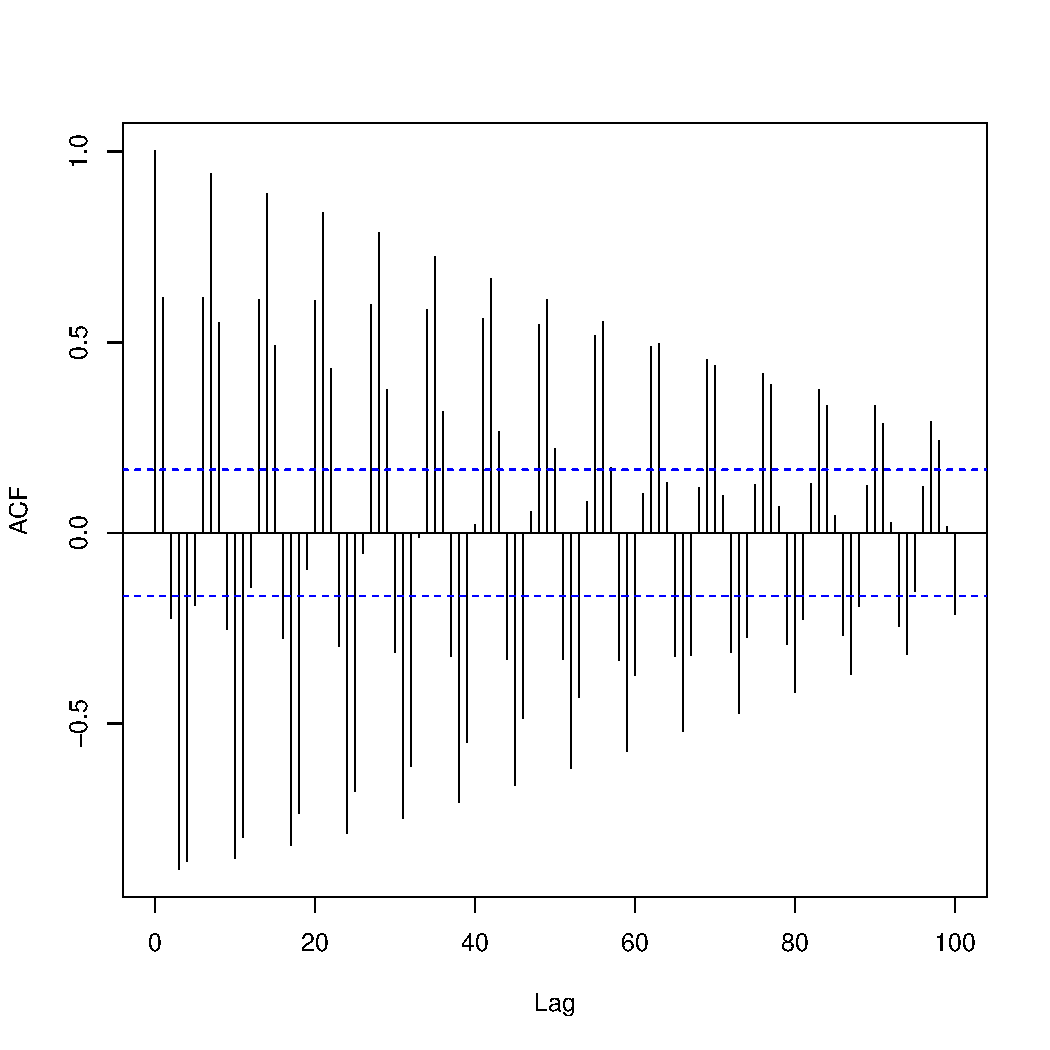
\includegraphics{img/acf-sine.pdf}}
            \caption{Autocorrelation function of sine function.}
            \label{img:period-acf}
        \end{center}
    \end{figure}

    The algorithm for automatic period identification is demonstrated in Algorithm \ref{alg:period-find}.
    It looks for periodically repeated significant values of ACF function. At some rate these values have to
    be decreased to zero. In the infinity ACF function converges to zero.

    The algorithm as input takes only time series. If there is a unit root present, then differencing is applied.
    Calculation of autocorrelation function of input time series follows and finding the index of its highest
    value. Then it checks if there are significant values of ACF present at following $n*period$ indices.
    There have to be present at lease two consecutive values of ACF, so $n$ takes values from $1,2,3\dots$

    \begin{algorithm}
        \caption{Find period of time series} \label{alg:period-find}
        \begin{algorithmic}[1]
        \Function{findFrequency}{$int[] ts$}
            \If{$unitRootPresent(ts)$} \Comment{e.g. ADF test}
                \State $ts \gets diff(ts)$ \Comment{first order differences}
            \EndIf
            \State $acf \gets acf(ts)$ \\
                        \Comment{returns index of the highest value}
            \State $period \gets findHighest(ts, period)$
            \While{$period * 2 < ts.length$}
                \If{$checkPeriodExists(x, ts)$}
                    \State \Return $period$
                \EndIf
              \State $period \gets findHighest(ts, period)$
            \EndWhile
            \State \Return $1$
        \EndFunction
        \end{algorithmic}
    \end{algorithm}

%%%%%%%%%%%%%%%%%%%%%%%%%%%%%%%%%%%%%%%%%%%%%%%%%%%%%%%%%%%%%%%%%%%
\chapter{Analytical Forecasting Process} \label{chap:models-demonstration}
In the previous chapter several time series models were described. However, in Hawkular only few of them were
selected and implemented.

This chapter demonstrates targeted models on real time series. There is also conducted a
statistical comparison of the models. This chapter also contains theory how different models should be compared. At
the end there is a discussion which models were selected for usage in Hawkular.

    %%%%%%%%
    \section{Evaluating Forecasting Accuracy} \label{sec:mse-mae}
    In order to evaluate a forecasts produced by particular model it is important to calculate the errors of the
    forecasts. There are several statistics for evaluating forecasting accuracy. The most used ones are mean squared
    error (MSE) \ref{eq:accuracy-mse} and mean absolute error (MAE) \ref{eq:accuracy-mae} \cite{statistika}. The
    difference between them is that MSE emphasizes the extremes while MAE is more robust to outliers
    \cite{hyndman-forecasting}.

    \begin{gather} \label{eq:accuracy-mse}
         MSE = \frac{1}{n} \sum_{i=1}^{n}(y_i - \hat{y_i}) \\
         MAE = \frac{1}{n} \sum_{i=1}^{n} \abs{y_i - \hat{y_i}} \label{eq:accuracy-mae}
    \end{gather}

    %%%%%%%%
    \section{Measuring Model Quality} \label{sec:model-quality}
    When comparing multiple models, statistics like MSE or MAE are not the best objective functions. Comparison
    based on this statistics can select complicated model with lots of parameters, which may overfit training data
    and most importantly it selects less robust model \cite{cipra}. Therefore for comparison multiple models another
    factors have to be added to the objective function. These factors are number of parameters of the model.

    The most used criteria for model sections are: Akaike information criterion (AIC) and Bayesian information
    criterion (BIC). Model with lower information criterion is preferred.

    \begin{gather} \label{eq:aic}
        AIC = 2 k - \ln(L) \\ \nonumber
        BIC = k \ln(n) - 2 \ln(L)
    \end{gather}

    Equations for AIC and BIC are listed in \ref{eq:aic}. Number of parameters of the model is represented by $k$.
    Number of observations is denoted by $n$ and $L$ stands for maximized value of the likelihood function of the
    model. In case for exponential smoothing it is minimized sum of squared error of one step ahead prediction of
    training data set.

    From the equations it can be seen that BIC penalizes models with more parameters. There is also AIC criterion with
    correction form \ref{eq:aicc}. Corrected version of AIC more penalizes longer models.

    \begin{eqnarray} \label{eq:aicc}
        AICc = AIC + \frac{2k(k+1)}{n-k-1}
    \end{eqnarray}

    %%%%%%%%
    \section{Models Demonstration} \label{sec:models-demonstration}
    An analytical process of modelling time series starts with plotting the data and fitting various models chosen by
    forecaster's previous experience. In second step forecaster compares statistics of those models and chooses the one
    that describes data the best.

    In this section real time series is modelled using time series models discussed in Chapter \ref{chap:models}.
    Chosen time series is \emph{austourists} from R package \texttt{fpp}. This series is a measurement of quarterly
    visitor nights spent by international tourists in Australia. It was chosen on purpose because it contains trend
    and seasonality.

    On the first Chart \ref{img:simple-models} there is depicted na\"{i}ve, average and drift model. Average model is
    just an overall average of the whole time series. It does not change over time. However there could be an online
    version of this algorithm for which an average would be calculated for each new value.

    Na\"{i}ve and drift model copy values of time series with lag of one observation. These two models differs in
    forecasts where drift model is capable of forecasting trends.

    \begin{figure}[H]
        \begin{center}
%            \resizebox{12cm}{8cm}{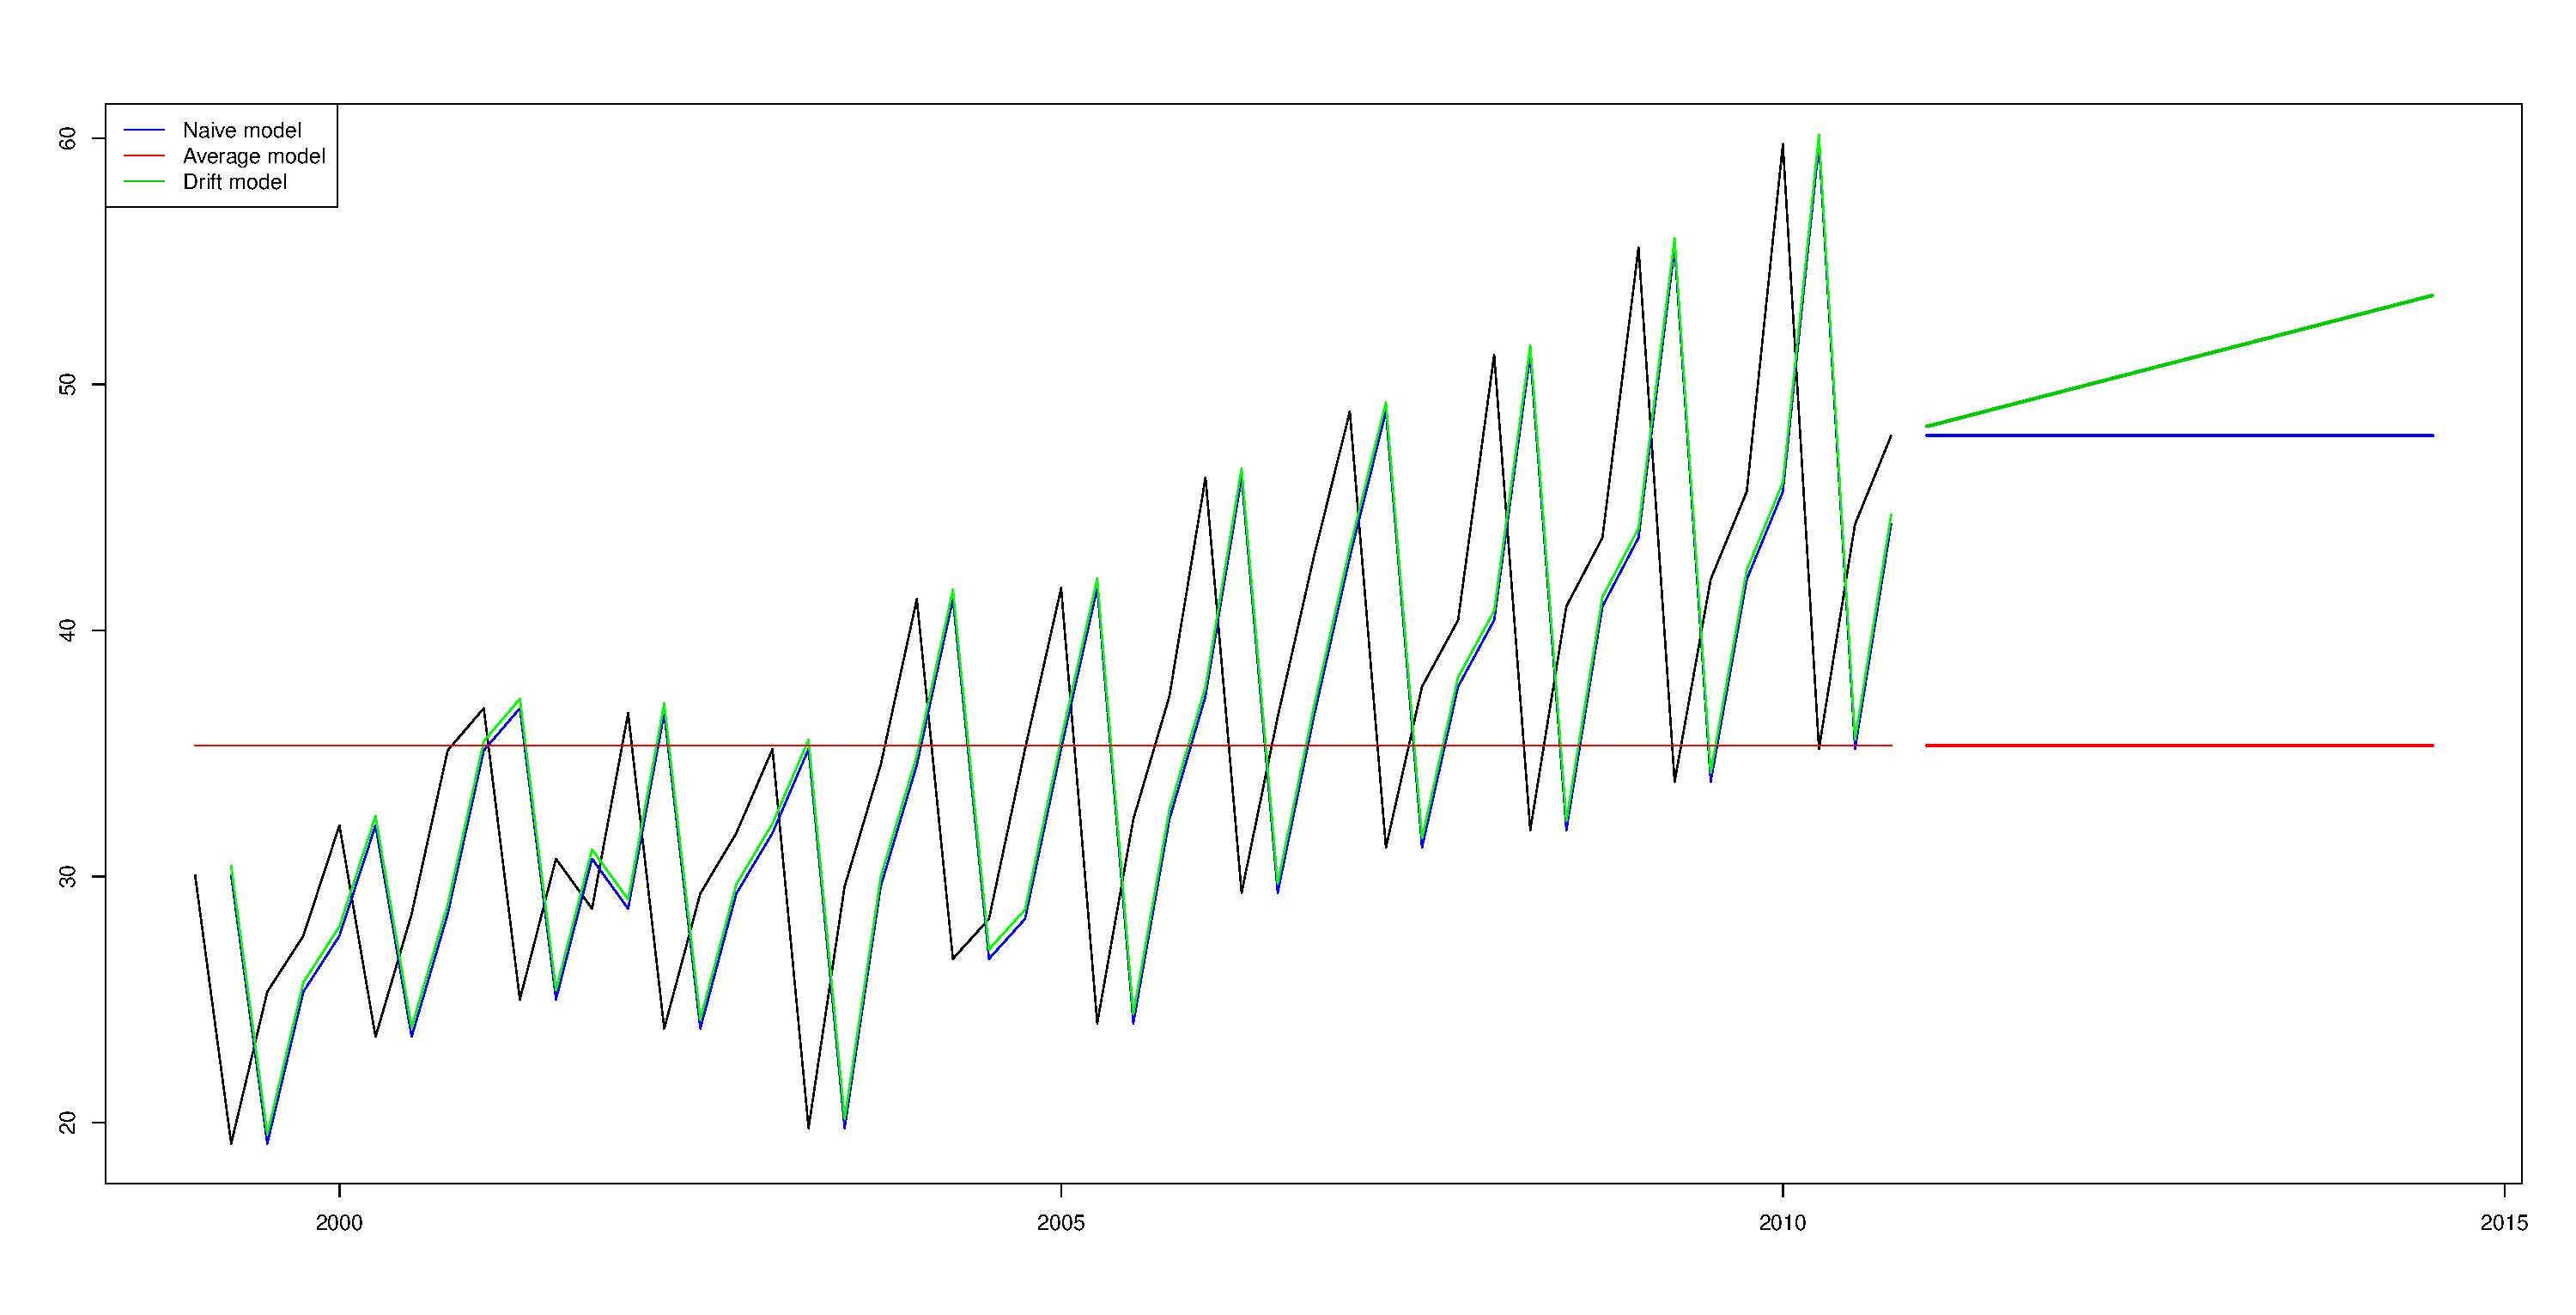
\includegraphics{img/simple-models.pdf}}
            \scalebox{0.255}[0.4]{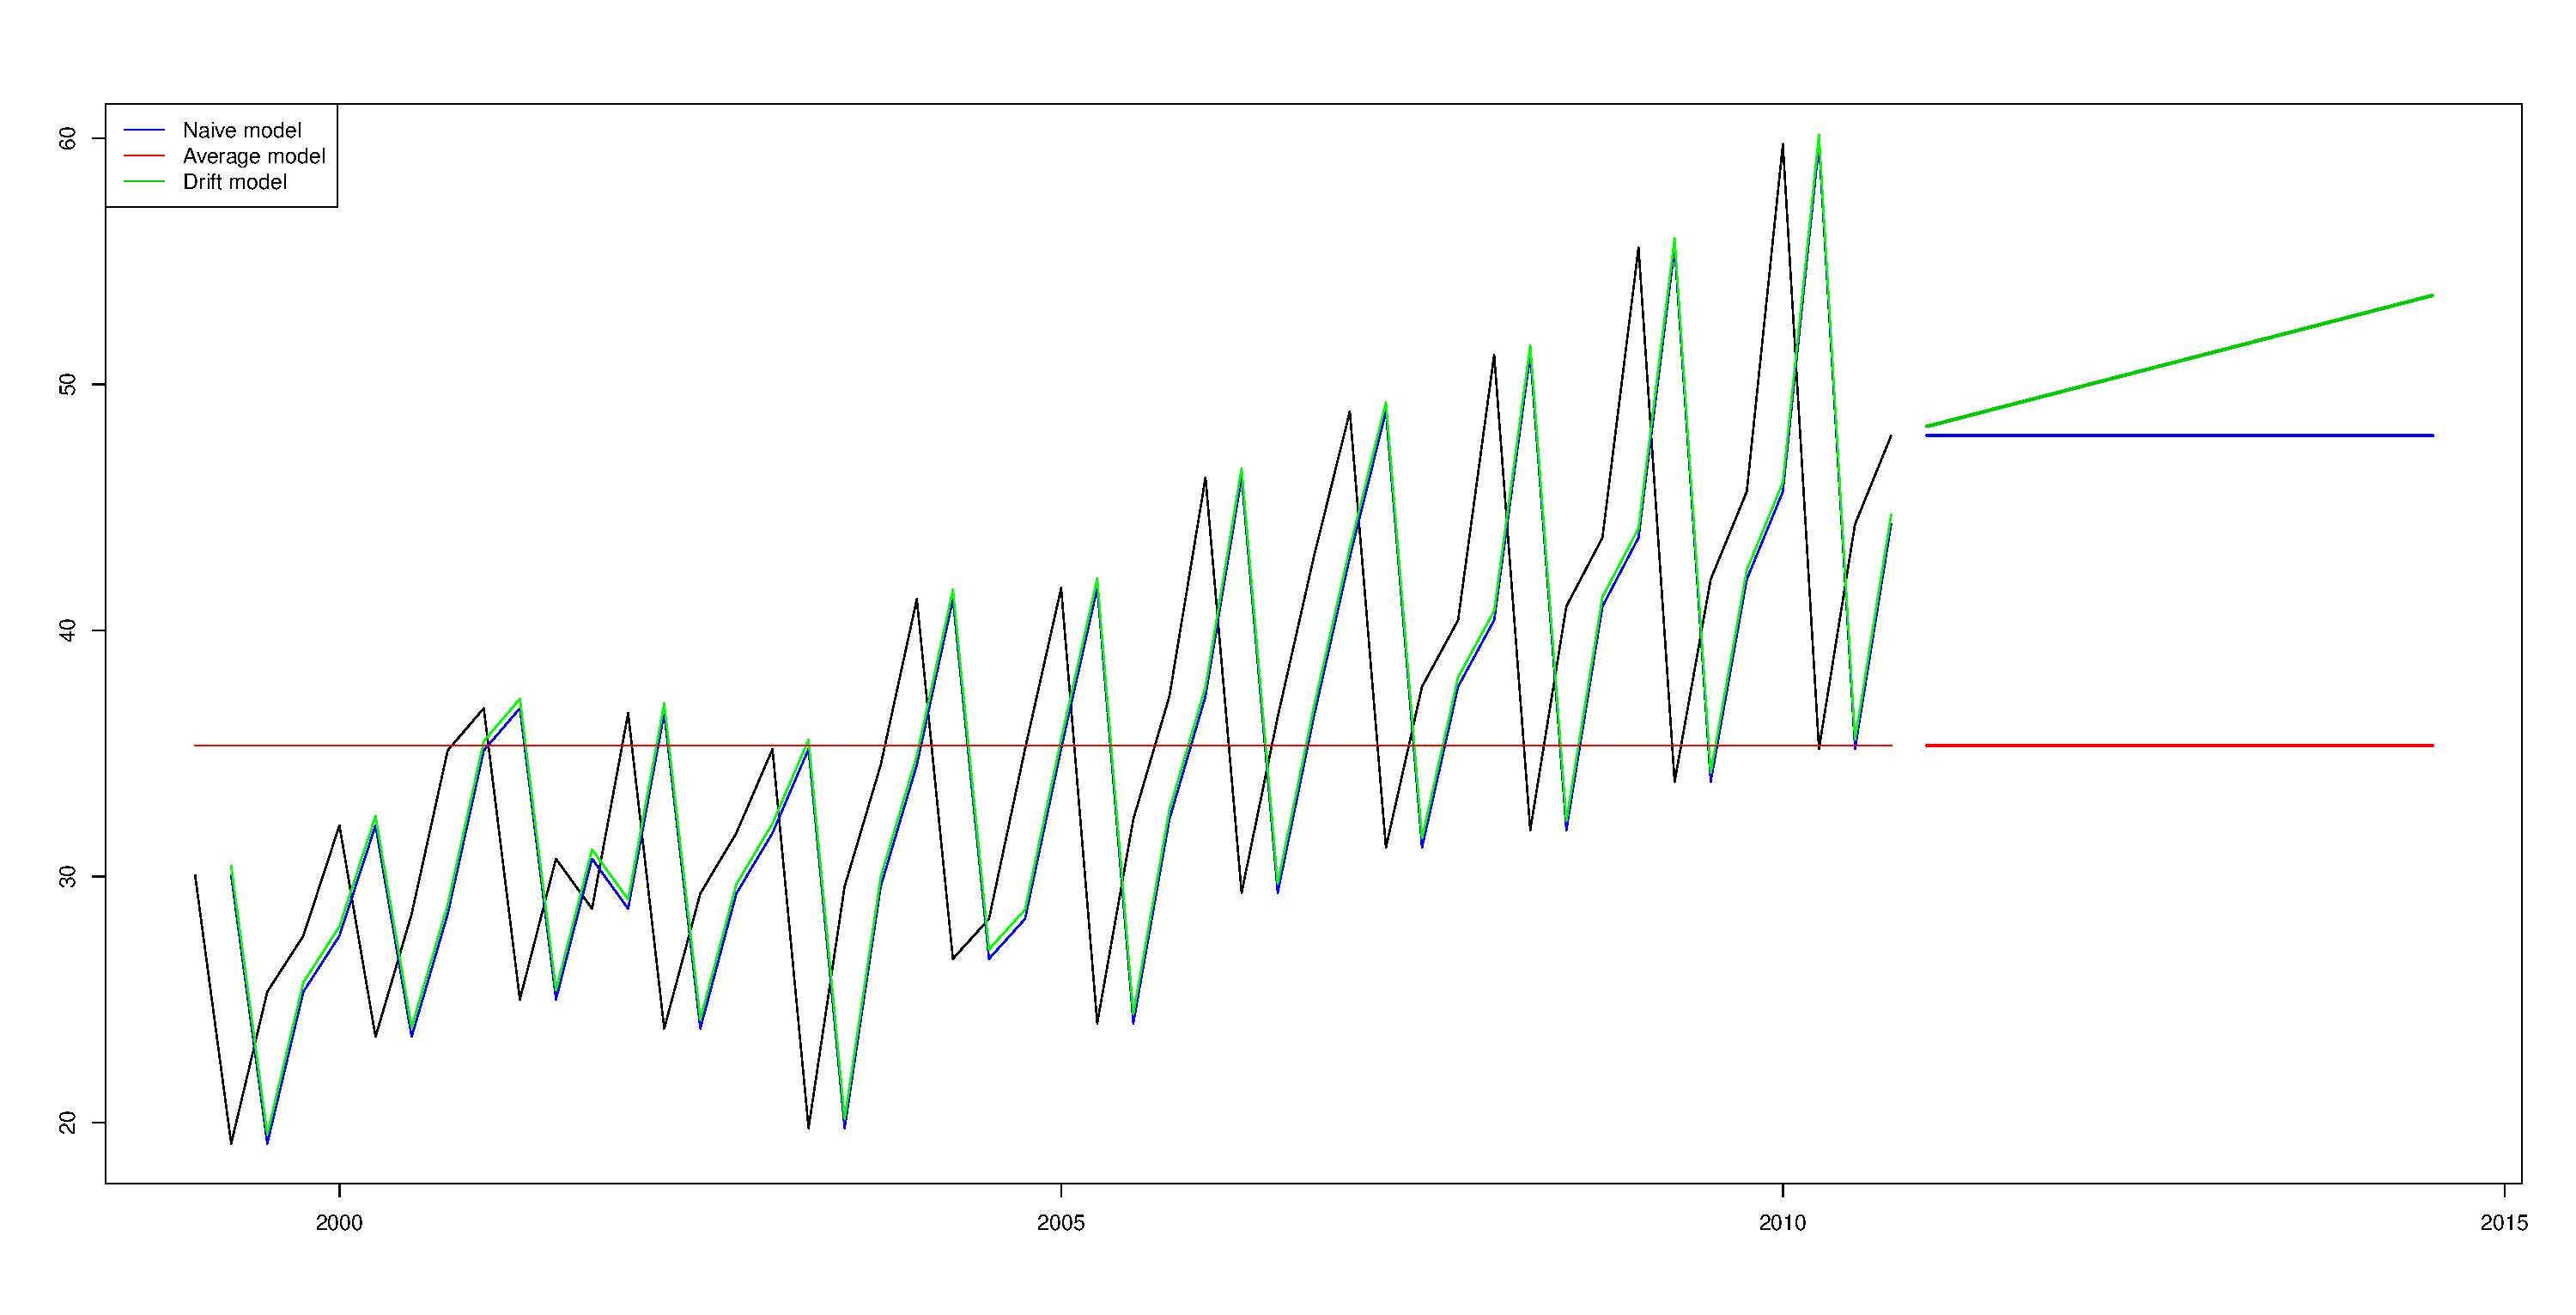
\includegraphics{img/simple-models.pdf}}
            \caption{Simple models on \emph{austourists}.}
            \label{img:simple-models}
        \end{center}
    \end{figure}

    Exponential smoothing models are depicted in Chart \ref{img:exp-smoothings}. For this particular series it is
    obvious that seasonal model is the best describing modelled time series.

    In the beginning it can be seen how is the seasonal model changing and learning the seasonal pattern from data.
    Learning and adaptivity to new trends depends on smoothing parameters of the models. Higher values of parameters
    allows the model quicker adapt to changes. Models with lower smoothing parameters are more robust to the changes.

    \begin{figure}[H]
        \begin{center}
            \scalebox{0.255}[0.27]{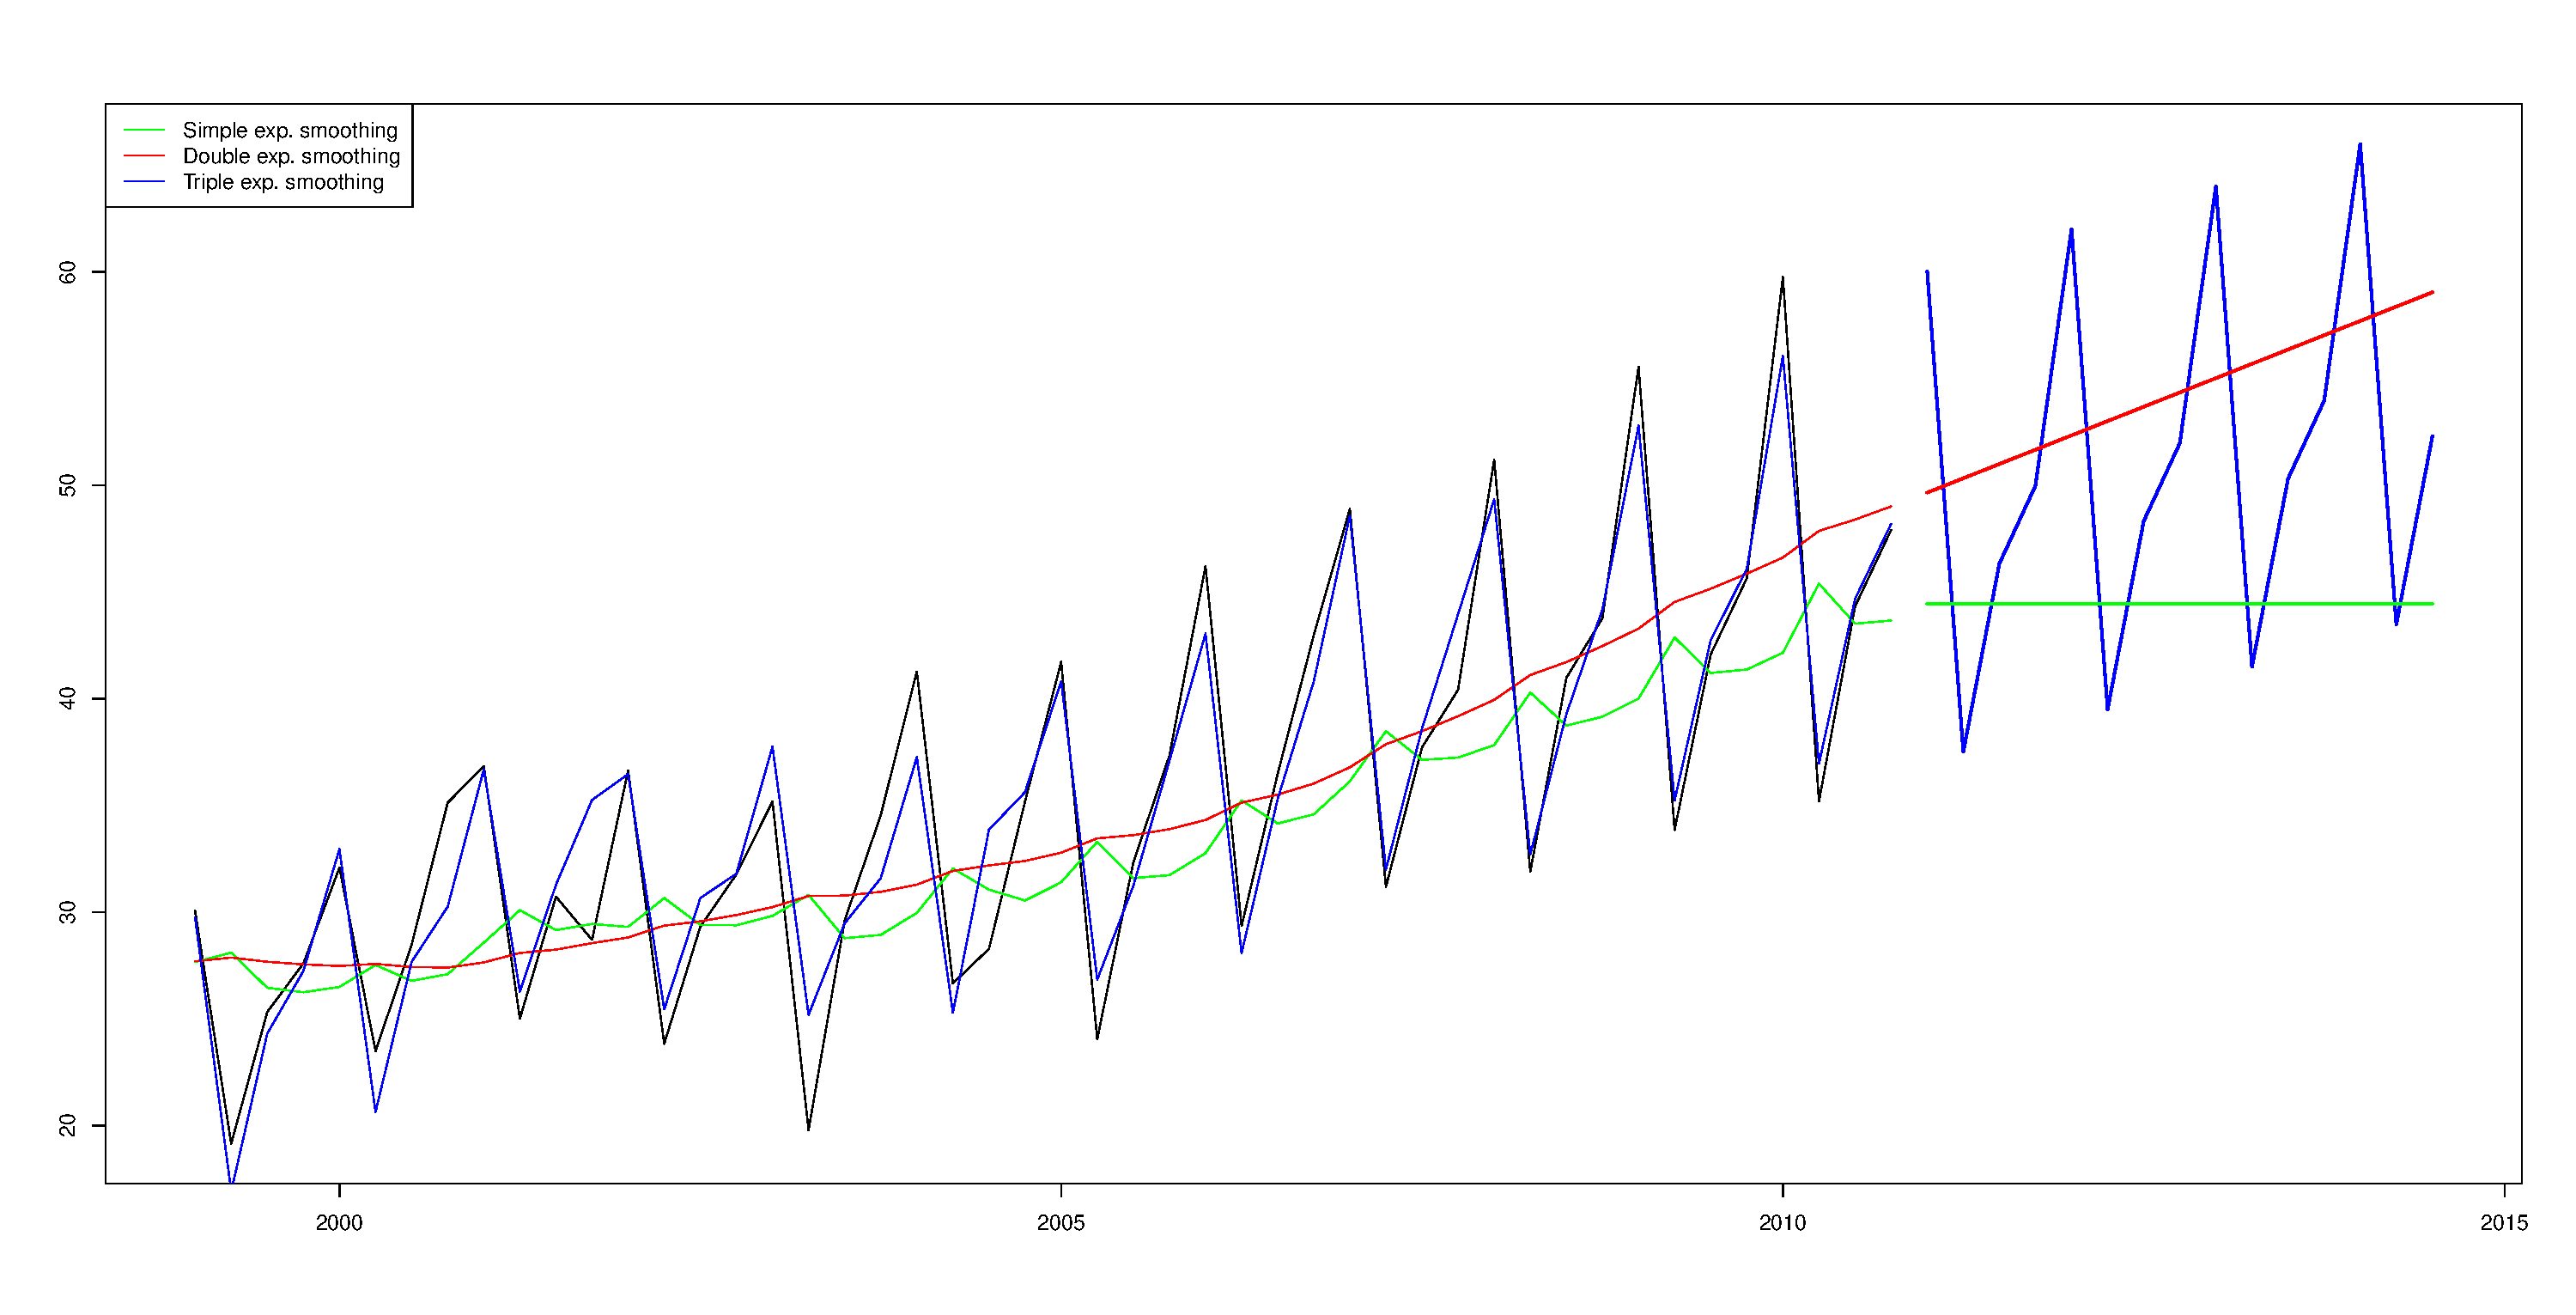
\includegraphics{img/exp-smoothings.pdf}}
            \caption{Exponential smoothing models on \emph{austourists}.}
            \label{img:exp-smoothings}
        \end{center}
    \end{figure}

    \begin{figure}[H]
        \begin{center}
            \scalebox{0.255}[0.27]{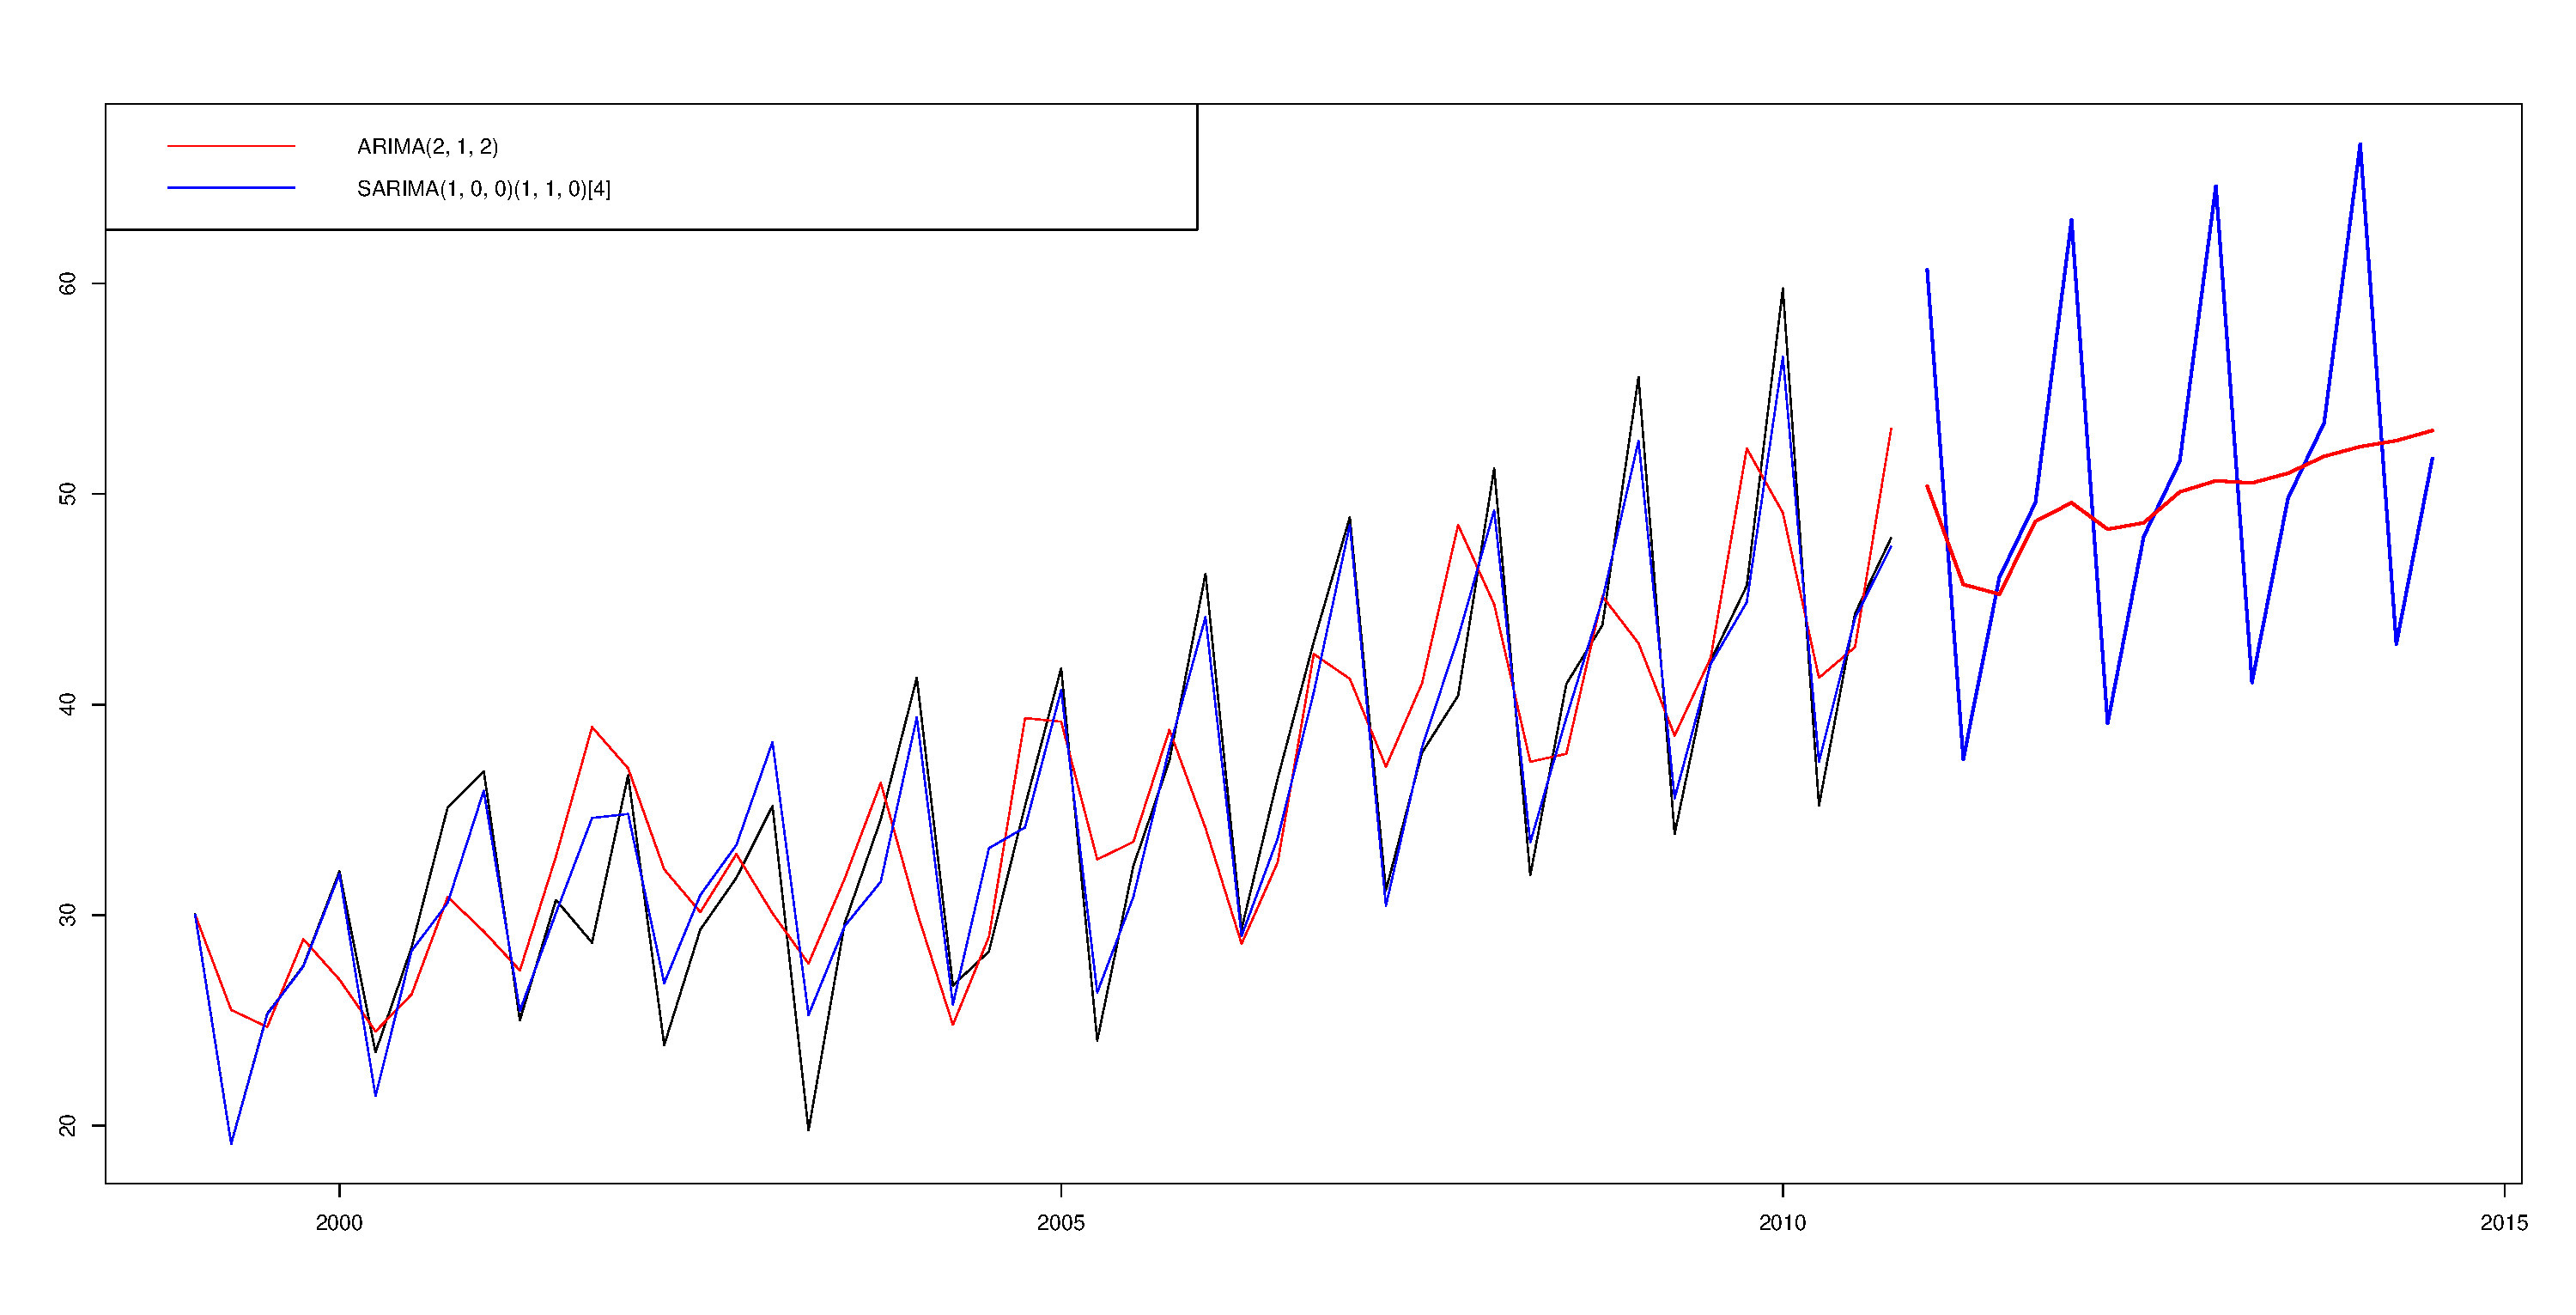
\includegraphics{img/arima-sarima.pdf}}
            \caption{Arima models on \emph{austourists}.}
            \label{img:arimas}
        \end{center}
    \end{figure}

    ARIMA models are shown in Chart \ref{img:arimas}. Non-seasonal model is already capable of capturing some seasonal
    patterns but it is more random whereas seasonal patterns should be of fixed period. Therefore seasonal ARIMA with
    dedicated model for each period is more appropriate.

    \begin{table}[h]
        \begin{center}
            \begin{tabular}{l|r|r|c}
                    \textbf{Model} & \textbf{MSE} & \textbf{MAE} & \textbf{AIC} \\ \hline \hline
                    Na\"{i}ve & 104.74 & 8.64 & \\
                    Drift & 104.60 & 8.47 & \\
                    Average & 79.91 & 7.14 & \\ \hline
                    Simple exp. smoothing & 53.54 & 5.91 & 380.88 \\
                    Double exp. smoothing & 44.41 & 5.28 & 375.90 \\
                    Triple exp. smoothing & 5.34 & 1.71 & 282.73 \\ \hline
                    Linear regression & 41.85 & 5.10 & 321.46 \\ \hline
                    ARIMA(2, 1, 2) & 30.88 & 4.35 & 310.6 \\
                    SARIMA(1, 0, 0)(1, 1, 0)[4] & 4.79 & 1.63 & 206.95 \\
            \end{tabular}
            \caption{Statistics of models.}
            \label{tab:models-stat}
        \end{center}
    \end{table}

    Statistics produced by each model are listed in Table \ref{tab:models-stat}. Models with the lowest one
    step ahead prediction error are seasonal ARIMA and triple exponential smoothing which is correct for this highly
    seasonal time series.

    As it was discussed in Section \ref{sec:model-quality} AIC criterion should be used for models comparison. From
    Table \ref{tab:models-stat} it can be seen that AIC and MSE are related, however MSE of double exponential smoothing
    is $8.3$ times higher than MSE of triple exponential smoothing, whereas AIC of double exponential smoothing is
    only $1.3$ times higher. From this example it is obvious how AIC discriminates models with more parameters.

%%%%%%%%%%%%%%%%%%%%%%%%%%%%%%%%%%%%%%%%%%%%%%%%%%%%%%%%%%%%%%%%%%%
\chapter{Existing Solutions}
Before going directly to the design and implementation let's briefly look at existing monitoring solutions and libraries
for time series modelling.

In the next section not only direct competitors of Hawkular are described but also
generally available software of this kind. Because Hawkular is still only an upstream project and not deliverable
product for the customers, thereby Jboss Operations Network (JON) is considered as its alternative.

However, this work does not focus on precise comparison of monitoring applications. It is only mentioned for wider
overview of this domain.

    %%%%%%%%
    \section{Monitoring and Management Applications}
    There are many monitoring solutions available out there. Some of them are offered as service (SaaS) and other need
    to be deployed in customer's environment.

    The most important features for each application are highlighted altogether with information how it differs from its
    competitors and if application offers predictive capabilities.

        %%%%%%%%
        \subsection{New Relic}
        New Relic was the first monitoring solution offered as SaaS \cite{new-relic}. It focuses on application
        performance rather than infrastructure view.

        Monitoring of Java applications is done by agents. Because agent manipulates with bytecode it is able to
        identify business transactions and monitor for instance utilization of REST endpoints.

        Agents also automatically discover databases connected to the application being monitored. From alert
        prediction perspective New Relic does not offer any alert prediction or predictive charts.

        %%%%%%%%
        \subsection{Dynatrace Ruxit}
        Ruxit is another popular SaaS solution for monitoring middleware applications. Monitoring is also done by agents
        which instrument bytecode so the application is also able to monitor business transactions. Ruxit differs from
        others in offering root cause analysis rather than firing multiple alerts \cite{ruxit}. It directly shows
        causing problems with visual representation. Ruxit does not offer any predictive alerting or charts.

        %%%%%%%%
        \subsection{Open Source Projects}
        As Hawkular is an open source project it is important to mention its direct competitors from this area.
        There are two major open source projects. The first one is Nagios and second Zabbix. Nagios was started in
        1991 and Zabbix in 2001 therefore both are more than fifteen years old.

        In comparison to Hawkular, Ruxit or New Relic the user interface of these two projects feels much older.
        At the time of writing this thesis last contribution to Nagios was from 17th September 2015 and Nagios
        project was active until the last moment. Both of these projects do not offer alert prediction.

        %%%%%%%%
        \subsection{HP OpenView and IBM Tivoli}
        The biggest monitoring solutions offered by these two software giants are HP OpenView and IBM Tivoli. Both are
        composed of many independent products. Solution from HP does not offer any predictive capabilities.

        Operations Analytics, one of IBM Tivoli products can automatically detect correlations between
        metrics which can lead to detection of application issues, for example an anomaly detection
        \cite{tivoli-predictive-insights}.

        Another part of Tivoli solution\,--\,Netcool Network Management is capable
        of predicting events. There is also another predictive analysis in Tivoli Monitoring
        module\footnote{Available at
        \url{https://www.ibm.com/developerworks/community/wikis/home?lang=en\#/wiki/Tivoli+Monitoring/}.}.
        In the online document there it is mentioned that predictive engine does not work on real time streams of data.
        Tivoli is definitely a big solution and in order to get real predictive capabilities it would require to
        contact IBM support.

    %%%%%%%%
    \section{Libraries For Time Series Forecasting} \label{sec:libraries-for-ts}
    In Java there is only one publicly available library for time series modelling. The library is called
    OpenForecast\footnote{Available at \url{http://www.stevengould.org/software/openforecast/index.shtml}.}. It contains
    models like na\"{i}ve, linear regression and exponential smoothing models. Whereas the library is open source, code
    was reviewed and tested. Some assumptions about the implementation were made. The parameters of some models are
    not estimated correctly. For example in linear regression slope and intercept are not estimated by minimizing
    sum of squared errors.

    The library provides nice feature called automatic forecaster which selects the best model for given
    time series, however the code produces null pointer exception. The bug was identified but the library is not
    maintained anymore.

    The performance of the library was also tested. Table \ref{tab:open-forecast-perf} contains execution times of
    optimizers for simple, double and triple exponential smoothing models. The tested time series is generated sine
    function of length 200 observations. The result is compared against execution times of R's function \texttt{ets}
    from \texttt{forecast} package.

    \begin{table}[h]
        \begin{center}
            \begin{tabular}{l|c|c}
                \textbf{Model} & \textbf{OpenForecast} & \textbf{R \texttt{forecast}} \\ \hline \hline
                Simple ex. & 4.91 sec. & 0.003 sec.\\
                Double ex. & 9.31 sec. & 0.006 sec.\\
                Triple ex. & 6.45 sec. & 0.209 sec.\\
            \end{tabular}
            \caption{Execution time of parameters estimation for exponential smoothing models.}
            \label{tab:open-forecast-perf}
        \end{center}
    \end{table}

    From the table it is obvious that R's implementation is much faster. For example optimization of thousand double
    exponential smoothing models would take about two and half hours. This results are not acceptable for Hawkular in
    real time environment.

    Another possibility is to directly use R implementation. There are various libraries\footnote{The most widely used:
    RCaller and JRI.} which allow executing R code from Java, however it requires installed R system in the target
    environment.

    Other possible solution is to use Rengin\footnote{Available at \url{http://www.renjin.org/}}\,--\,JVM interpreter
    for R. However \texttt{forecast} package depends on other package which invocates native C++ code for optimized
    computations. Therefore \texttt{forecast} package can not be used with Rengin.

%%%%%%%%%%%%%%%%%%%%%%%%%%%%%%%%%%%%%%%%%%%%%%%%%%%%%%%%%%%%%%%%%%%
\chapter{Design and Implementation} \label{chap:design-impl}
The module for an alert prediction is named Hawkular Data Mining. Source code is versioned in Git and
hosted on Github\footnote{Available at \url{https://github.com/hawkular/hawkular-datamining}.} under
license Apache version 2.0.

The project is split into several Maven artifacts. This approach decomposes problem into smaller parts
which have dedicated functionality and can be easy reused in other projects. It also ensures that
third party dependencies are loaded only for certain artifacts, where are needed.

Figure \ref{appen:maven-deps} shows dependency tree of \texttt{datamining-dist}, which is the top level artifact.
The most important modules are listed in Table \ref{tab:datamining-modules}. All ids of the listed artifacts have prefix
\texttt{hawkular-datamining}.

\begin{table}[h]
    \begin{center}
        \begin{tabular}{l|l}
            \textbf{Artifact Id} & \textbf{Description} \\ \hline \hline
            \texttt{parent} & Manages shared dependencies and versions. \\
            \texttt{forecast} & Core library for time series modeling and forecasting. \\
            \texttt{api} & API used within Data Mining. \\
            \texttt{cdi} & Support for context dependency injection. \\
            \texttt{rest} & Web archive for standalone usage without Hawkular. \\
            \texttt{dist} & Web archive with Hawkular integration code. \\
            \texttt{itest} & Artifact for integration tests.
        \end{tabular}
        \caption{Hawkular Data Mining modules.}
        \label{tab:datamining-modules}
    \end{center}
\end{table}

In the following sections the most important parts of the implementation are described. This text focuses on
design of data structures, interaction between them and algorithms.

    %%%%%%%%
    \section{Forecast Package}
    The forecast package is time series modelling and forecasting library. It contains several time series models
    and utility classes for time series modelling. It is designed to be easy used in any Java project. \\The footprint
    of the artifact is small. It depends only on Apache Math, Commons, Guava and Jboss logging.

    The core data structures from \texttt{datamining-forecast} package are interfaces of time series models
    and forecasters. Some of the methods are listed in Algorithm \ref{alg:models}. These two interfaces are related but
    not the same. Each time series model should be capable of predicting and learning. Models also collect
    initialization and running statistics so it is possible to make assumptions of the forecasting accuracy.

    The main difference between forecaster and time series model is that forecaster is designed for online learning
    and it autonomously selects the most appropriate time series model. Time series models by default are not
    designed for online learning, however it can be accomplished with a wrapper class.

    Metric in the Data Mining is represented as structure \texttt{MetricContex} which contains metadata like
    collection interval, metric id and tenant id. Collection interval is necessary for calculating timestamps of
    predicted points.

    \begin{lstlisting}[caption={Interface for time series models.}, language=Java, label={alg:models}]
interface TimeSeriesModel {
    void learn(List<DataPoint> ts);
    List<DataPoint> forecast(int steps);
    int numberOfParameters();
    MetricContext context();
    AccuracyStatistics initStatistics();
    AccuracyStatistics runStatistics();
    ...
     }
    \end{lstlisting}

    List of implemented models, statistical and utility classes for time series manipulation:

    \begin{multicols}{2}
        \begin{itemize}
            \item Simple ex. smoothing
            \item Double ex. smoothing
            \item Triple ex. smoothing
            \item Weighted moving average
            \item Automatic forecaster
            \item Augmented Dickey\,--\,Fuller test
            \item Time series decomposition
            \item Autocorrelation function
            \item Time series lagging
            \item Time series differencing
            \item Automatic period identification
        \end{itemize}
    \end{multicols}

        %%%%%%%%
        \subsection{Automatic Forecaster}
        One of the most important forecasting classes in Data Mining is \\\texttt{AutomaticForecaster}. This class
        autonomously decides which time series model should be used for modelled time series. Currently it decides from
        three implemented models: simple, double and triple exponential smoothing. Other models which implement
        interface \\\texttt{TimeSeriesModel} can be easily added.

        Most importantly, this class is capable of dealing with concept drift. It holds circular buffer of historical
        metrics and if statistical properties of the underlying time series changes content of the buffer is used for
        selecting new model.

        The strategy when a new model should be selected is configurable. The system currently
        supports two strategies. The first strategy selects new model periodically each $n$ observations.
        The second one is more sophisticated and it selects a new model only when the error produced on learning data
        exceeds by $x\%$ error calculated on learning points when model was initialized.

        Model selection is based on information criterion from Section \ref{sec:model-quality}. Automatic forecaster in
        successive steps calls optimizers of given models and then selects the best with the lowest information
        criterion. Used criterion is configurable for each forecaster.

        %%%%%%%%
        \subsection{Model Optimizers}
        Model optimizers are the most important part of the models implementation. If the model parameters are not
        estimated correctly, model produces high forecasting error.

        The idea behind optimization is to find such
        parameters that describe training data the best \cite{hyndman-state-space}. Optimization criterion can be: mean
        squared error, mean absolute error and likelihood. These criterion basically computes errors produced by ahead
        predictions. The number of prediction steps depends on the forecaster's objective. The most common is to use
        only one step ahead. Data Mining currently supports only MSE criterion but others can be easy added.

        The criterion is returned from model's objective function. This objective function is then passed to non-linear
        optimization algorithm from Apache Math Commons. This library implements several optimization algorithms:
        Nelder-Mead simplex, multi-directional simplex and bound optimization by quadratic approximation (BOBYQA).
        These algorithms do not need computed derivatives of the cost function.

        In terms of the lowest execution time and quality of the estimated parameters the best results were produced by
        Nelder-Mead simplex algorithm.

        Table \ref{tab:open-forecast-perf} contains comparison of optimizers execution times from \texttt{OpenForecast}
        and R implementation. This section adds execution time of Data Mining implementation. Complete execution times
        are listed in Table \ref{tab:datamining-perf}. Execution times of Data Mining's optimizers are in some
        cases faster than R. Quality of the produced forecasts is discussed in Chapter \ref{chap:evaluation}.

        \begin{table}[h]
            \begin{center}
                \begin{tabular}{l|c|c|c}
                    \textbf{Model} & \textbf{OpenForecast} & \textbf{R \texttt{forecast}} &
                        \textbf{Data Mining}\\ \hline \hline
                    Simple ex. & 4.91 sec. & 0.003 sec. & 0.033 sec.\\
                    Double ex. & 9.31 sec. & 0.006 sec. & 0.002 sec. \\
                    Triple ex. & 6.45 sec. & 0.209 sec. & 0.023 sec. \\
                \end{tabular}
                \caption{Execution time of parameters estimation for exponential smoothing models.}
                \label{tab:datamining-perf}
            \end{center}
        \end{table}

    %%%%%%%%
    \section{API Package}
    The next package is \texttt{api}. It depends on \texttt{forecast} and it eventually could
    depend on another library for data analysis, for instance a library for an outlier detection. In this package there
    is a code necessary for using Data Mining as application which analyzes multiple metrics, for example classes for
    accessing data analysis objects for given metric.

    The interface \texttt{SubscriptionManager} was designed for accessing time series analysis objects. Some of its
    methods are listed in Algorithm \ref{alg:sub-manager}. Implementation of this interface could store entities in
    database. However, Data Mining directly does not use any database. Therefore \\ \texttt{SubscriptionManager}
    holds all objects in memory. Internally it stores objects in a map where the key is tenant and value another
    map where the key is metric id and value the object for data analysis\,--\,\texttt{Subscription}.

    \begin{lstlisting}[caption={Interface \texttt{SubscriptionManager}.}, language=Java, label={alg:sub-manager}]
interface SubscriptionManager {
     void subscribe(Subscription, Owner);
     void unsubscribe(tenant, metric, Owner);
     Subscription model(tenant, metric);
     ...
     }
    \end{lstlisting}

    For subscribing it is necessary to specify the owner of the prediction configuration. It was specially added for
    integration with Inventory. It is more described in Section \ref{sec:dist}.

    Object \texttt{Subscription} holds instance of \texttt{AutomaticForecaster} and it could also hold another
    data analysis objects. Its role is to delegate calls to the business logic objects.

    Class diagram of the most important classes from \texttt{forecast} and \texttt{api} is depicted in Appendix
    \ref{appen:class-diagram}.

    Some of the service classes like \texttt{SubscriptionManager} are used in several other classes and also multiple
    implementation could exist (in memory or database implementation). Therefore dependency injection
    design pattern was introduced. Used technology is Java context dependency injection (CDI). In order to keep
    API classes clean module \texttt{cdi} with CDI configuration was introduced. It directly depends on \texttt{api},
    but does not add any other business logic.

    %%%%%%%%
    \section{REST Package}
    Package \texttt{rest} contains implementation of REST services provided by Data Mining. Implementation is
    compatible with standard JAX-RS.

    Data Mining REST API is designed to operate on the forecasting engine. When the module is deployed into Hawkular
    main interaction with Data Mining goes through Inventory REST API and metric data are collected from JMS topic.
    However, this is not limited and Data Mining offers alternative REST endpoints which can be used for
    example in standalone deployment.

    REST API provides following capabilities:

    \begin{itemize}
        \item Operate on subscriptions\,--\,enable and disable prediction.
        \item Push learning data to the engine.
        \item Get predictions for any number of steps ahead.
        \item Configure automatic forecaster.
        \item Get information about model being used and statistics of the predictions.
    \end{itemize}

    Accurate and more comprehensive REST API documentation is available on Hawkular web page\footnote{Available at
    \url{http://www.hawkular.org/}.}. This documentation is automatically generated using Swagger framework.

    %%%%%%%%
    \section{Distribution Package\,--\,Integration into Hawkular} \label{sec:dist}
    As it was mentioned before, the build produces two web archives, one for standalone usage and another for
    deployment into Hawkular. The second web archive adds extra functionality for interacting with the other Hawkular
    components.

    In Hawkular all entities are stored in Inventory, therefore Data Mining uses this module
    for querying metric definitions and it adds some extra attributes necessary for predictions. Another module
    \\which is used by Data Mining is Hawkular Metrics. Diagram \ref{img:hawkular-interaction} shows Data Mining
    integration into Hawkular.

    \begin{figure}[H]
        \begin{center}
            \scalebox{0.32}{\includegraphics{img/src/architecture.pdf}}
            \caption{The integration into Hawkular.}
            \label{img:hawkular-interaction}
        \end{center}
    \end{figure}

    When Data Mining is deployed into Hawkular, users can enable predictions by creating Relationship\footnote{Entity
    from Inventory which can be created between arbitrary two entities.} from tenant to the target entity. Target
    entity can be metric, metric type or tenant. When relationship is created from tenant to tenant, predictions are
    enabled for all metrics under given tenant. Similarly, when a target entity is a metric type, predictions are
    enabled for all metrics of that type. In Figure \ref{img:relationship} is depicted part of the structure of
    inventory with enabled predictions.

    Relationships also store properties needed for predictions. One of them is forecasting horizon which tells how
    many prediction steps are performed for each incoming metric data point. With this approach of storing
    relationships in Inventory, Data Mining does not have to use any database for entities related to predictions.
    This approach was achieved without any changes to Inventory data model, this shows that Inventory's generic data
    model build on top of graph database\footnote{Compatible with Apache Tinkerpop.} is good approach for storing data
    model in this domain.

    \begin{figure}[H]
        \begin{center}
            \scalebox{0.35}{\includegraphics{img/src/inventory.pdf}}
            \caption{Relationship between entities of Inventory.}
            \label{img:relationship}
        \end{center}
    \end{figure}

    Any changes in Inventory are propagated to Data Mining by subscribing to specific events. This propagation is done
    through JMS topic where Inventory sends these events. However, on application start Data Mining also needs to query
    all predictive relationships from Inventory. For this purpose JMS request-response communication was implemented in
    Inventory. Any component which has access to internal messaging subsystem can construct a query and send it for
    execution to Inventory. REST API approach was also proposed but it could expose vulnerability\,--\,client
    could access any data objects of any tenant. Diagram \ref{img:sequence-enab-pred} depicts sequence of calls
    when prediction gets enabled.

    \begin{figure}[H]
        \begin{center}
            \scalebox{0.30}[0.20]{\includegraphics[angle=0]{img/src/uml-enable-predictions-sequence.pdf}}
            \caption{Sequence diagram of enabling predictions.}
            \label{img:sequence-enab-pred}
        \end{center}
    \end{figure}

    From Diagram \ref{img:sequence-enab-pred} it is clear that when a prediction gets enabled, historical metrics
    are queried from Metrics module. This means that Data Mining needs to access metrics of all tenants. It is
    similar scenario to getting all predictive relationships from Inventory. It could not be implemented via REST API
    because of potential vulnerability and JMS based query was rejected by Metrics developers.

    Another two solutions were proposed. The first was to bypass Metrics and query data directly from Cassandra.
    The second was to inject Metrics as CDI bean and directly use its Java API. The first solution was refused because
    the schema is maintained by Metrics and it can eventually change and also the backed database (Cassandra) can
    change. The final and implemented solution injects Metrics as CDI bean. This approach assumes that Metrics
    are deployed in the same application server as Data Mining. From the performance perspective it is faster that
    JMS or REST calls.

    Diagram \ref{img:sequence-incoming-data} shows complete data flow from agent to alerts evaluation engine.
    First metric data is sent by agent to Metrics where it is stored to database. Then it is sent to JMS topic
    and consumed by Alerts and Data Mining. In parallel Alerts evaluates alerts criteria and Data Mining computes
    predictions. After computation the predicted data are sent back to the same JMS topic and consumed by Alerts.
    At this point an alert of predicted metrics can be triggered.

    Data Mining changes \texttt{id} of predicted points in order to be able to distinguish original time series from
    predicted. For predicted metrics Alerts can evaluate the same conditions as for original time series or use
    different ones, more in Section \ref{sec:alerts-conditions}.

    \begin{figure}[H]
        \begin{center}
            \scalebox{0.33}[0.24]{\includegraphics[angle=0]{img/src/uml-incoming-data-sequence.pdf}}
            \caption{Sequence diagram of incoming data from agent.}
            \label{img:sequence-incoming-data}
        \end{center}
    \end{figure}

        %%%%%%%%
        \subsection{Alerts and Conditions} \label{sec:alerts-conditions}
        In this section it is briefly described how the alerting system works. Alerts is a separate module
        which is responsible for firing alerts based on defined conditions. As it is depicted in Diagram
        \ref{img:sequence-incoming-data} Alerts listens to the JMS topic and if conditions for given metric are
        positively evaluated an alert is fired.

        Alerts data model is little bit more complicated though, as for each unique metric id multiple conditions can be
        defined. These conditions are evaluated for every received metric data point on the bus. Conditions are
        grouped under a trigger. If the result of evaluation is positive than the trigger triggers an action. This
        action can be for instance sending an email, sms or perform a webhook\dots

        Triggers can be grouped which facilitates creation of the similar triggers. Particularly this can be used for
        creating triggers for predictive metrics. If there is a trigger defined for the original metric it can be
        duplicated and used for predicted metrics.

        If necessary the conditions can be changed in
        order to not trigger an alert if the predictions are not very accurate. Trigger dampening can be used for this.
        So for the trigger which operates on predicted metrics dampening can be set as follows: \emph{``fire an alert if
        $X$ consecutive evaluations of conditions are positive``}.

        %%%%%%%%
        \subsection{Hawkular UI}
        Predictive charts in Hawkular are located in Metric explorer tab. In Figure \ref{img:hawkular-explorer}
        predictive chart for metric accumulated garbage collection duration is shown. In this case automatic
        forecaster decided to use seasonal model of some automatically identified period. Note that for displaying
        original time series in the chart buckets were used, so the periods would be more easily seen on raw data
        points.

        \begin{figure}[H]
            \begin{center}
%                \scalebox{0.33}[0.24]{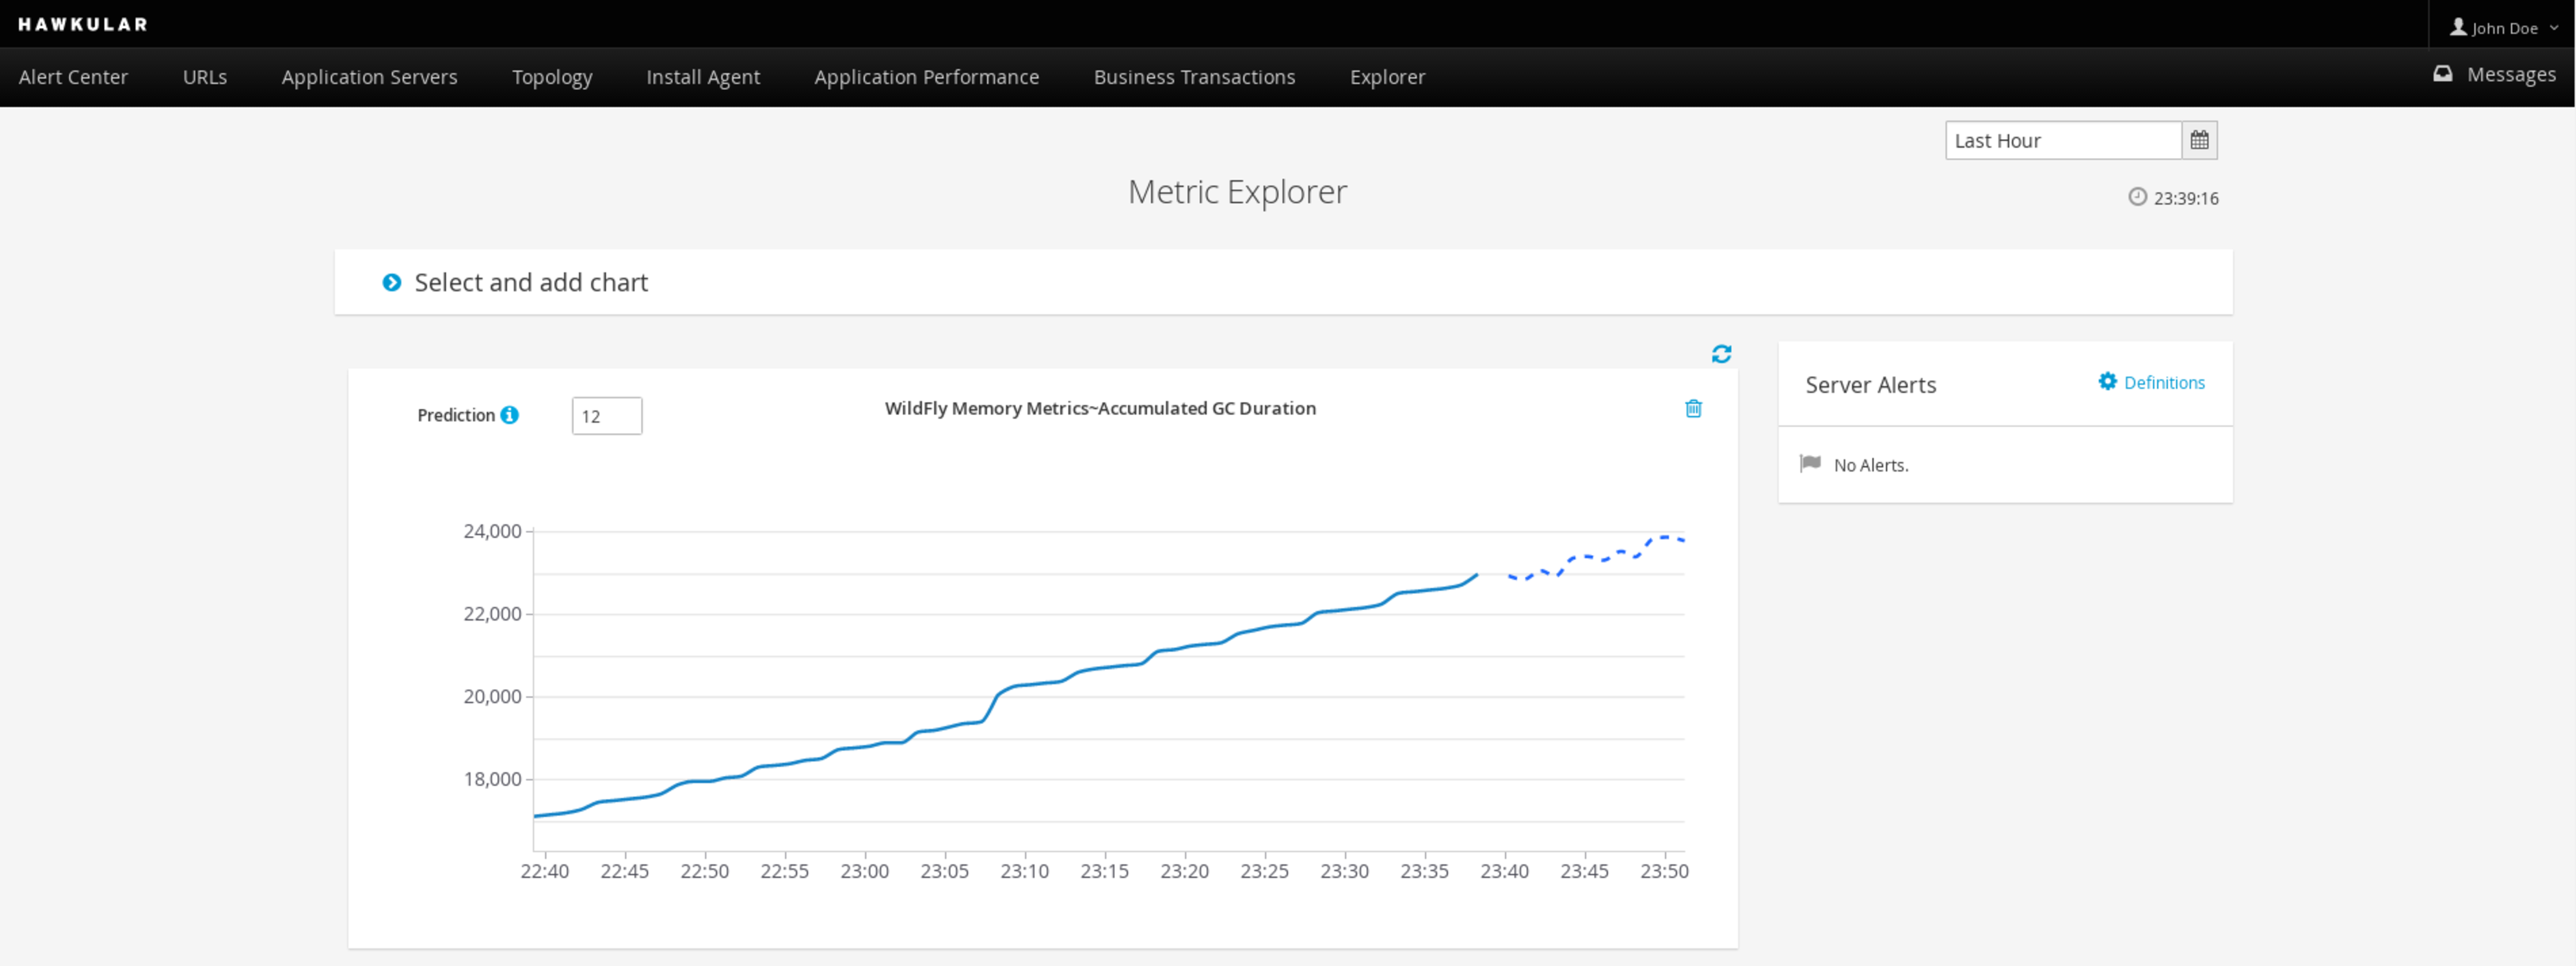
\includegraphics[angle=0]{img/hawkular-explorer.pdf}}
                \scalebox{0.185}[0.28]{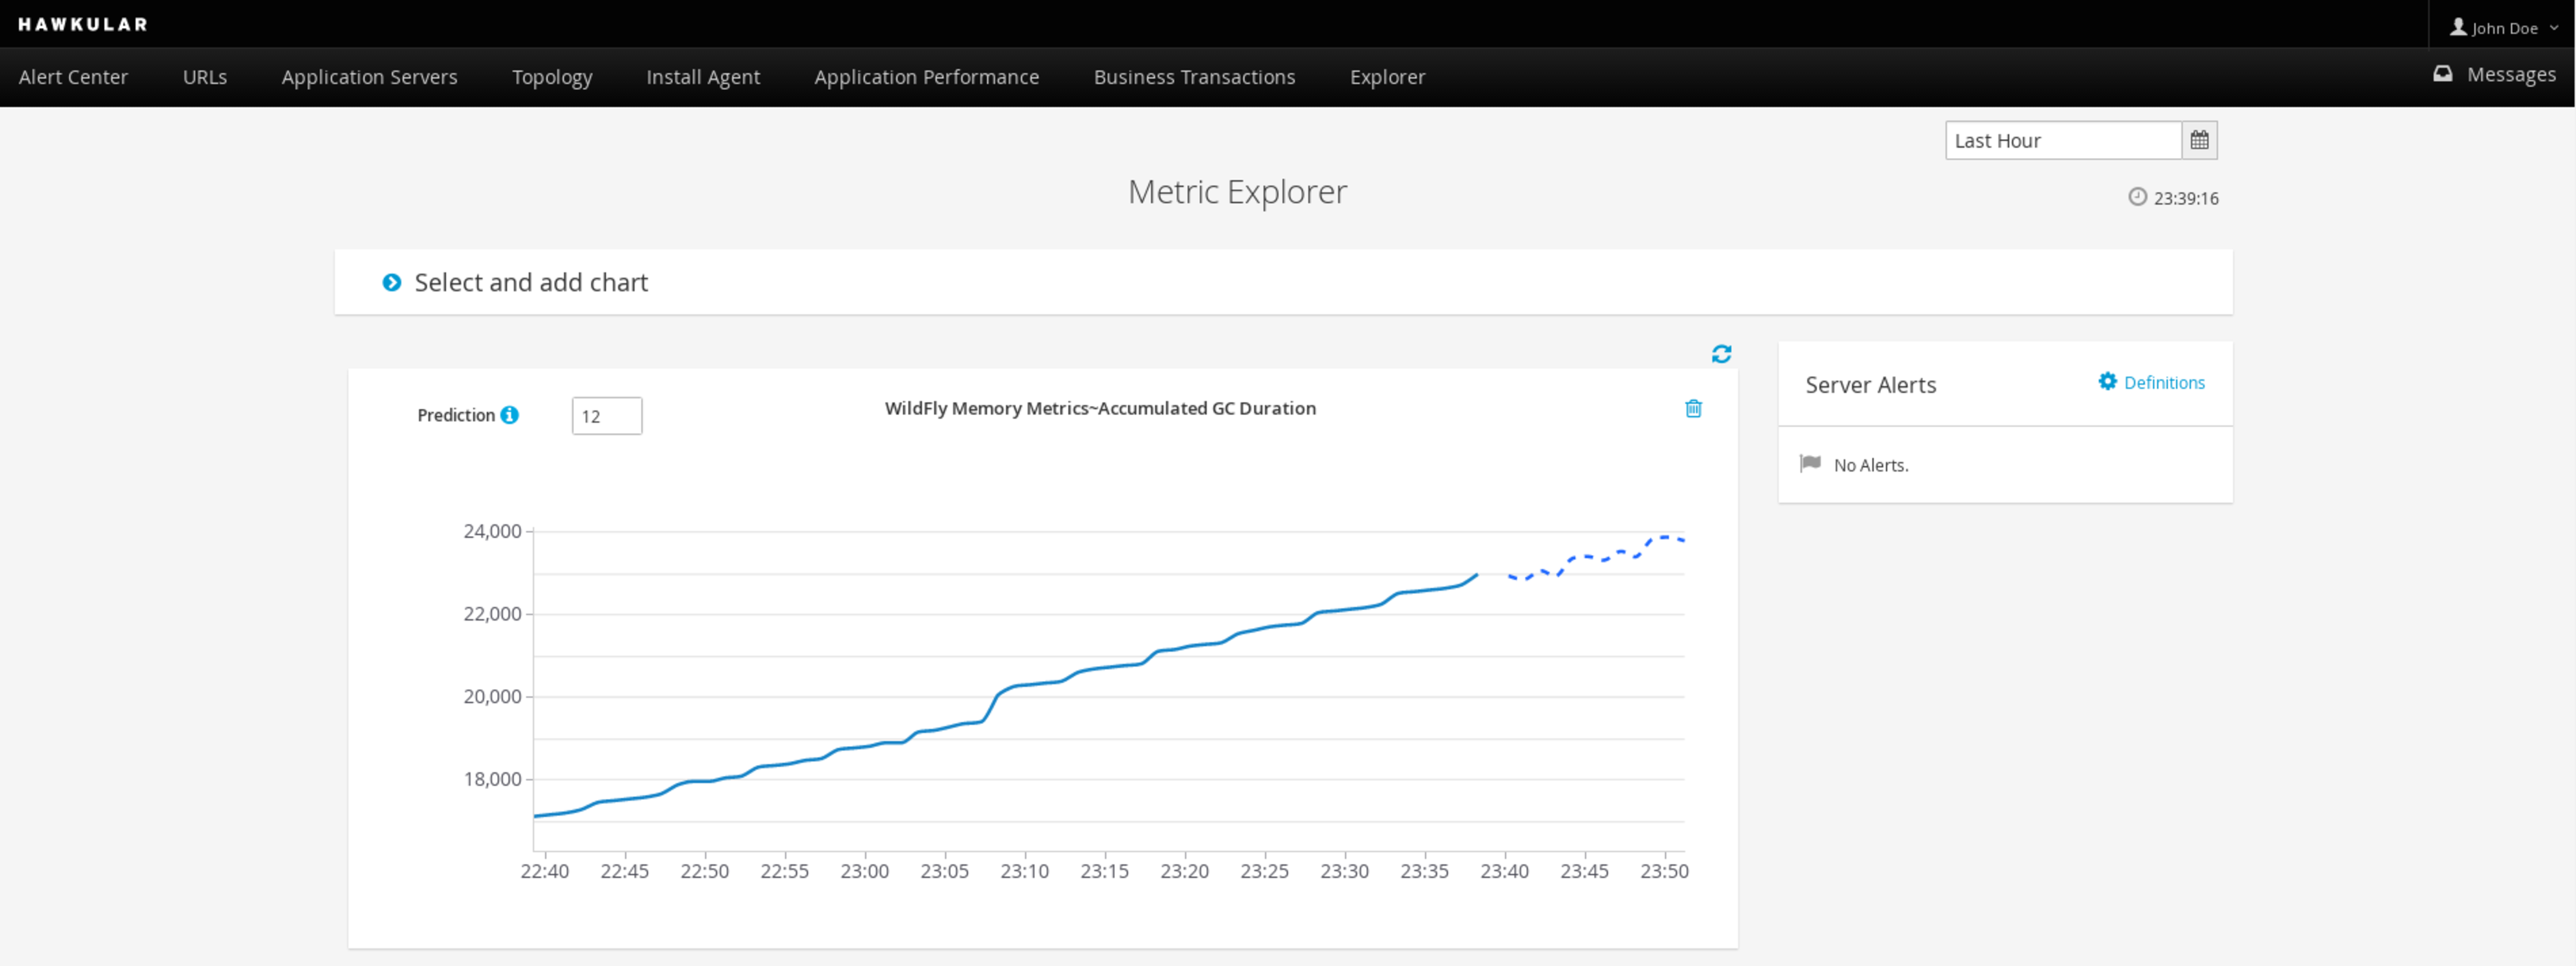
\includegraphics[angle=0]{img/hawkular-explorer.pdf}}
                \caption{Metric explorer tab in Hawkular user interface.}
                \label{img:hawkular-explorer}
            \end{center}
        \end{figure}

        After adding concrete chart predictions can be enabled by increasing prediction horizon input.
        So there is no need to enable predictions manually by creating relationship in Inventory.

        Predictive charts were used from repository \texttt{hawkular-charts}. These charts are built on top of
        D3\footnote{Avalilable at \url{https://d3js.org/}.} library and encapsulated as Angular directives.

    %%%%%%%%
    \section{Test Automation and Documentation}
    Core functionality of the application is covered by unit tests. Junit framework is used for this type of tests.
    Because Data Mining interacts with other applications and modules, integration tests are also implemented. These
    tests are executed from Maven profile which starts web server with necessary modules deployed.

    The last type of implemented tests are end-to-end tests which call REST endpoint of one module and expect result
    in call from another module. These types of tests are also executed in Maven profile with running web server.
    End-to-end tests for Data Mining project live in the main Hawkular integration repository\footnote{
    Available at \url{https://github.com/hawkular/hawkular}.}.

    All tests are automatically executed every time developer creates a pull request or pushes code to the master
    branch. For this Travis continuous integration platform was used, which is available for free for open source
    projects on Github.

    Documentation is directly written in Java code as javadoc. REST API documentation is also directly
    written in source code using Swagger framework and automatically generated at build time
    \footnote{Available at \url{http://www.hawkular.org/docs/rest/rest-datamining.html}.}.

    %%%%%%%%
    \section{Releases}
    At the time of writing this thesis, there was only one release with version \texttt{0.1.Final}. It is also available
    in the Maven central repository. Complete group id is \texttt{org.hawkular.datamining}. The most important
    artifact ids are listed in Table \ref{tab:datamining-modules}. Release notes are available on
    Github\footnote{Available at \url{https://github.com/hawkular/hawkular-datamining/releases}.}.

    %%%%%%%%
    \section{Retrospective}
    In this section it is mentioned how the project was changing during the implementation, what did not worked well and
    what could have been done better.

    At the beginning of the project Apache Spark\footnote{Open source cluster computing framework available at
    \url{https://spark.apache.org/}.} was used for building regression models. Its machine learning library (MLIB)
    offers several learning algorithms. In Data Mining linear regression with stochastic gradient descent was used.
    Because the gradient is stochastic, produced predictions are not very robust and quickly change by significant
    value.

    Spark was mainly used because of its streaming extension that can handle
    high-throughput stream data \cite{apache-spark}. There is also time series library
    \texttt{spark-ts}\footnote{Available at \url{https://github.com/sryza/spark-timeseries}.} which contains some
    time series models but does not offer functionality of automatic model selection.

    Due to the problems with linear regression discussed in Section \ref{sec:linear-regression} and lack of automatic
    forecaster, decision was made to drop Spark and directly implement exponential smoothing models.

    During the implementation a lot of time was spent on integration with other modules, with Inventory in particular.
    The problem was that Inventory is developed by another party and any concrete document
    describing the integration was not proposed. The design of the integration was understood differently
    by both parties, which lead to reimplementing of some parts. Therefore it is better to precisely define the
    integration interface with other modules or projects.

%%%%%%%%%%%%%%%%%%%%%%%%%%%%%%%%%%%%%%%%%%%%%%%%%%%%%%%%%%%%%%%%%%%
\chapter{Evaluation of Implemented Models} \label{chap:evaluation}
Evaluation process compares predictive capabilities of the implemented models to statistics produced by similar models
from R language. Models from R language are selected because they are widely used by forecasters all around the
world and de facto standard for statistical science \cite{kleiber2008applied}, therefore, for this work considered
as referential.

To be specific used models are from package
\texttt{forecast}\footnote{Available at \url{https://cran.r-project.org/web/packages/forecast/index.html}.}.
Function used for fitting models is \texttt{ets}. This function accepts several configuration parameters for instance:
what model should be used, statistics for objective function, information criterion\dots For testing in this work model
parameter is set to \texttt{ANN}, \texttt{AAN} and \texttt{AAA} for simple, double and triple exponential smoothing,
objective statistics for minimization is MSE and parameter damped set to false.

The used methodology and more comprehensive description of tested objectives is listed in Section \ref{sec:methodology}.

    %%%%%%%%
    \section{Methodology} \label{sec:methodology}
    In order to evaluate forecasting quality of the implemented models it is necessary to use well defined
    methodology with test data which contains broad range of patterns: white noise, monotonicity, random
    shocks, trend and seasonality.

    Most importantly methodology should not evaluate forecasting accuracy how well model
    fits the historical data. Instead it should evaluate forecast accuracy using genuine forecasts\,--\,test
    how well \\model performs on new data \cite{otexts}. Therefore it is necessary to split time series into training
    and test set.

    The size of the test set is usually 20\% of the total sample. Albeit the size of test set depends on how
    long all the sample is and how far ahead one wants to forecast.
    \newpage
    Outline of the methodology used in this work:
    \begin{enumerate} \label{enum:methodology}
        \item Divide data sample into training and test set.
        \item Set $k = size(trainingSet)$.
        \item Train model on the training set. And learn up to $k^{th}$ observation. \label{item:train}
        \item Compute n-step ahead forecast $\hat{y}$ and error $\epsilon = y-\hat{y}$.
        \item Set $k = k+1$ and continue at step \ref{item:train} until $k=size(trainingSet + testSet)$.
        \item Calculate MSE of produced errors.
    \end{enumerate}

    As it was described earlier time series used for testing should contain one or even combine more patterns together.
    Test samples used in this work are depicted in Appendix \ref{appen:testing-samples}. Each sample contains white
    noise, random shocks and one or more of the following patterns: monotonicity, trend and seasonality. Names and
    description of test samples are listed in Table \ref{tab:test-samples-description}.

    \begin{table}[h]
        \begin{center}
            \begin{tabular}{l|l}
                \textbf{Time Series Name} &  \textbf{Description} \\ \hline \hline
                \texttt{wn} & Constant white noise. \\
                \texttt{trendUpLow} & Upward trend with white noise. \\
                \texttt{trendDownHigh} & Downward trend of high variance. \\
                \texttt{sine} & Constant sine with white noise. \\
                \texttt{sineTrend} & Sine with trend and white noise. \\
            \end{tabular}
            \caption{Description of test samples.}
            \label{tab:test-samples-description}
        \end{center}
    \end{table}

    The last part what figures in our methodology is training size. Let's say that one would like to forecast one hour
    ahead and Wildfly Agent collects most of the metrics in five minute intervals. Thus forecasting horizon of one
    hour corresponds to 12 observations and training set should be at least long 48 observations.

    Interesting is also to find out if forecasting accuracy changes for larger training set. Therefore it
    was decided to add training sets of length 100 and 200 observations.

    In the following sections each model is tested using methodology from Section \ref{enum:methodology} on
    samples from Table \ref{tab:test-samples-description} of training size of 48, 100 and 200 observations with
    forecasting horizon set to: 1, 6 and 12 steps ahead. The size of test set is always 12 observations.

    Following notation is used to identify test cases:
    \begin{itemize}
        \item \emph{trainSampleSize\,--\,testSampleSize (forecastingHorizon)}
    \end{itemize}
    So for instance 48\,--\,12(1) denotes: training sample of size 48 observations, 12 test observations and
    forecasting horizon 1 step ahead.

    %%%%%%%%
    \section{Results}
    Complete test results are listed in Appendix \ref{appen:chap:results}. The top value in each cell is the result
    from R and below is the result from Data Mining. All measured values are in mean squared error. The table contains
    lot of data, however this work focuses on answering these two questions:

    \begin{enumerate}
        \item \emph{How well do the Data Mining models perform compared to R models?} \label{itm:question2}
        \item \emph{Does the size of training set affect quality of the forecasts?} \label{itm:question1}
    \end{enumerate}

    The first question can be answered by calculating ratios of Data Mining MSE to R MSE. If the ratio is lower than
    one it means that Data Mining model forecast more accurately.

    From the test results it can be shown how many tests cases have lower ratio or even better it is to split ratios
    into following intervals:
    lower than 1, \interval[{1,1.01}], \interval[{1.01,1.05}], \interval[{1.05,1.10}], \interval[{1.1,1.2}]
    and higher than 1.2. More aggregated representation is to calculate averages of these ratios for each test case.

    In order to get the answer for the second question it is necessary to compare MSE statistics produced by Data
    Mining models. For instance compare the result of test case 48\,--\,12(1) on \texttt{wn} sample to the same test
    case but with longer training set and analogously for other test samples and longer forecasting horizons. With
    this approach there would be too many results to compare. So this work first calculates averages of mean squared
    error of each test case, so the average for 48\,--\,12(1) is the average of all test samples (\texttt{wn},
    \texttt{trendUpLow}\dots) \\ of given test case.

    Chart with clear results is constructed for each of these two questions. The results of these charts are
    described in the following sections.

        %%%%%%%%
        \subsection{Simple Exponential Smoothing} \label{sec:results-simple}
        Raw results for simple exponential smoothing are listed in Table \ref{appen:tab:simple-results}.
        Pie Chart \ref{img:results-simple-pie} shows that Data Mining simple exponential smoothing model produces
        lower MSE than R in 38\% of all forty-five test cases and 38\% tests results are equal or worse at mosts than
        1\%. The test with worst result has 8\% higher MSE than equivalent R model.

        Data Mining's best result has 23\% lower MSE than the result from R model. It is for test case 100\,--\,12(1)
        on test sample \texttt{trendUpLow}.

        \begin{figure}[H]
            \begin{center}
                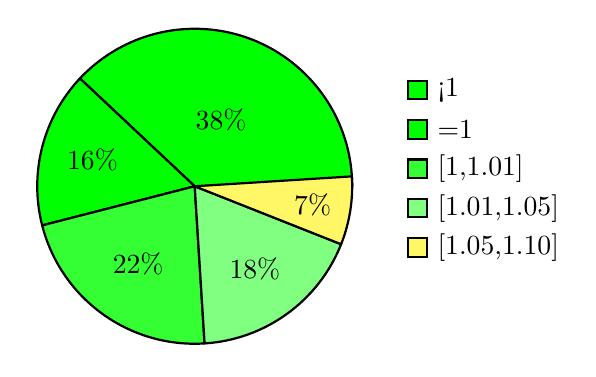
\begin{tikzpicture}
                    \pie[text=legend, radius=2, color={green!100 , green!100, green!80, green!50, yellow!60}]
                    {38/<1,
                    16/=1,
                    22/\interval[{1,1.01}],
                    18/\interval[{1.01,1.05}],
                    7/\interval[{1.05,1.10}]}
%                    0/ \interval[{1.1,1.2}],
%                    0/ >1.2}
                \end{tikzpicture}
                \caption{The proportion of Data Mining MSE to R MSE ratios split into intervals.}
                \label{img:results-simple-pie}
            \end{center}
        \end{figure}

        Chart \ref{img:results-simple-r} shows average ratios of Data Mining MSE to R MSE for each test case. These
        results are finer variants of results from Chart \ref{img:results-simple-pie}. It highlights that only three
        test cases out of nine have in average higher MSE than R and at most 2\% higher. It also shows that for
        larger training set Data Mining simple exponential smoothing in average produces lower MSE than R and
        on shorter training set R produces lower MSE than Data Mining.

        \begin{figure}[H]
            \begin{center}
                \scalebox{0.65}[0.45]{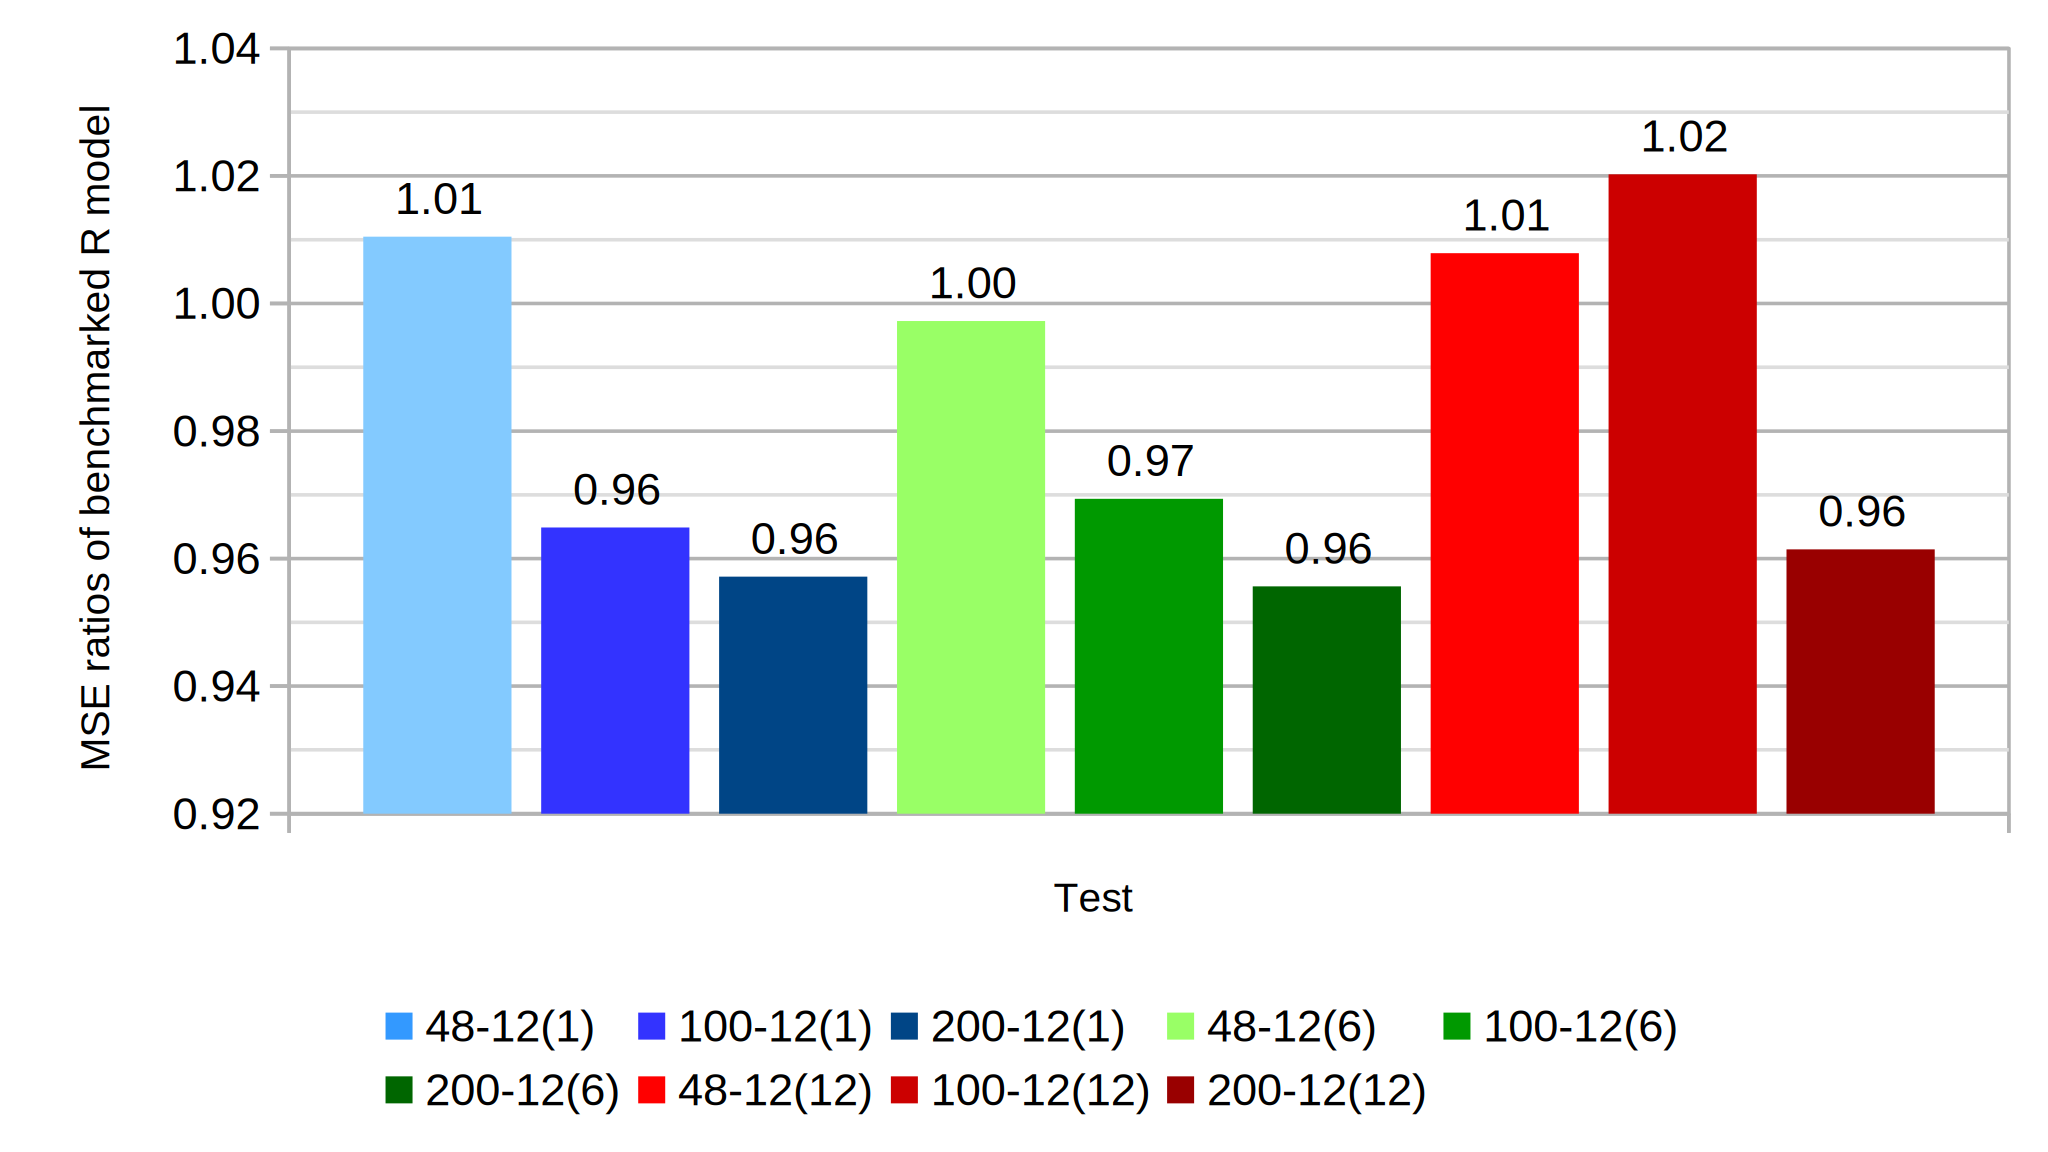
\includegraphics[angle=0]{img/src/results-simple-r.pdf}}
                \caption{Test results for triple exponential smoothing. Comparison to reference R model.}
                \label{img:results-simple-r}
            \end{center}
        \end{figure}

        Averages for each test case of Data Mining MSE are listed in Chart \ref{img:results-simple-mse}. This chart
        shows that the lowest average MSE are produced in test cases with training size of 48 observations. Therefore
        for simple exponential smoothing it is not necessary to use longer training set in order to get lower prediction
        error. Note that training samples contains randomly generated shocks. Therefore if more shocks are located later
        in time series than test cases for larger training sample can have higher MSE.

        \begin{figure}[H]
            \begin{center}
                % width, height
                \scalebox{0.65}[0.44]{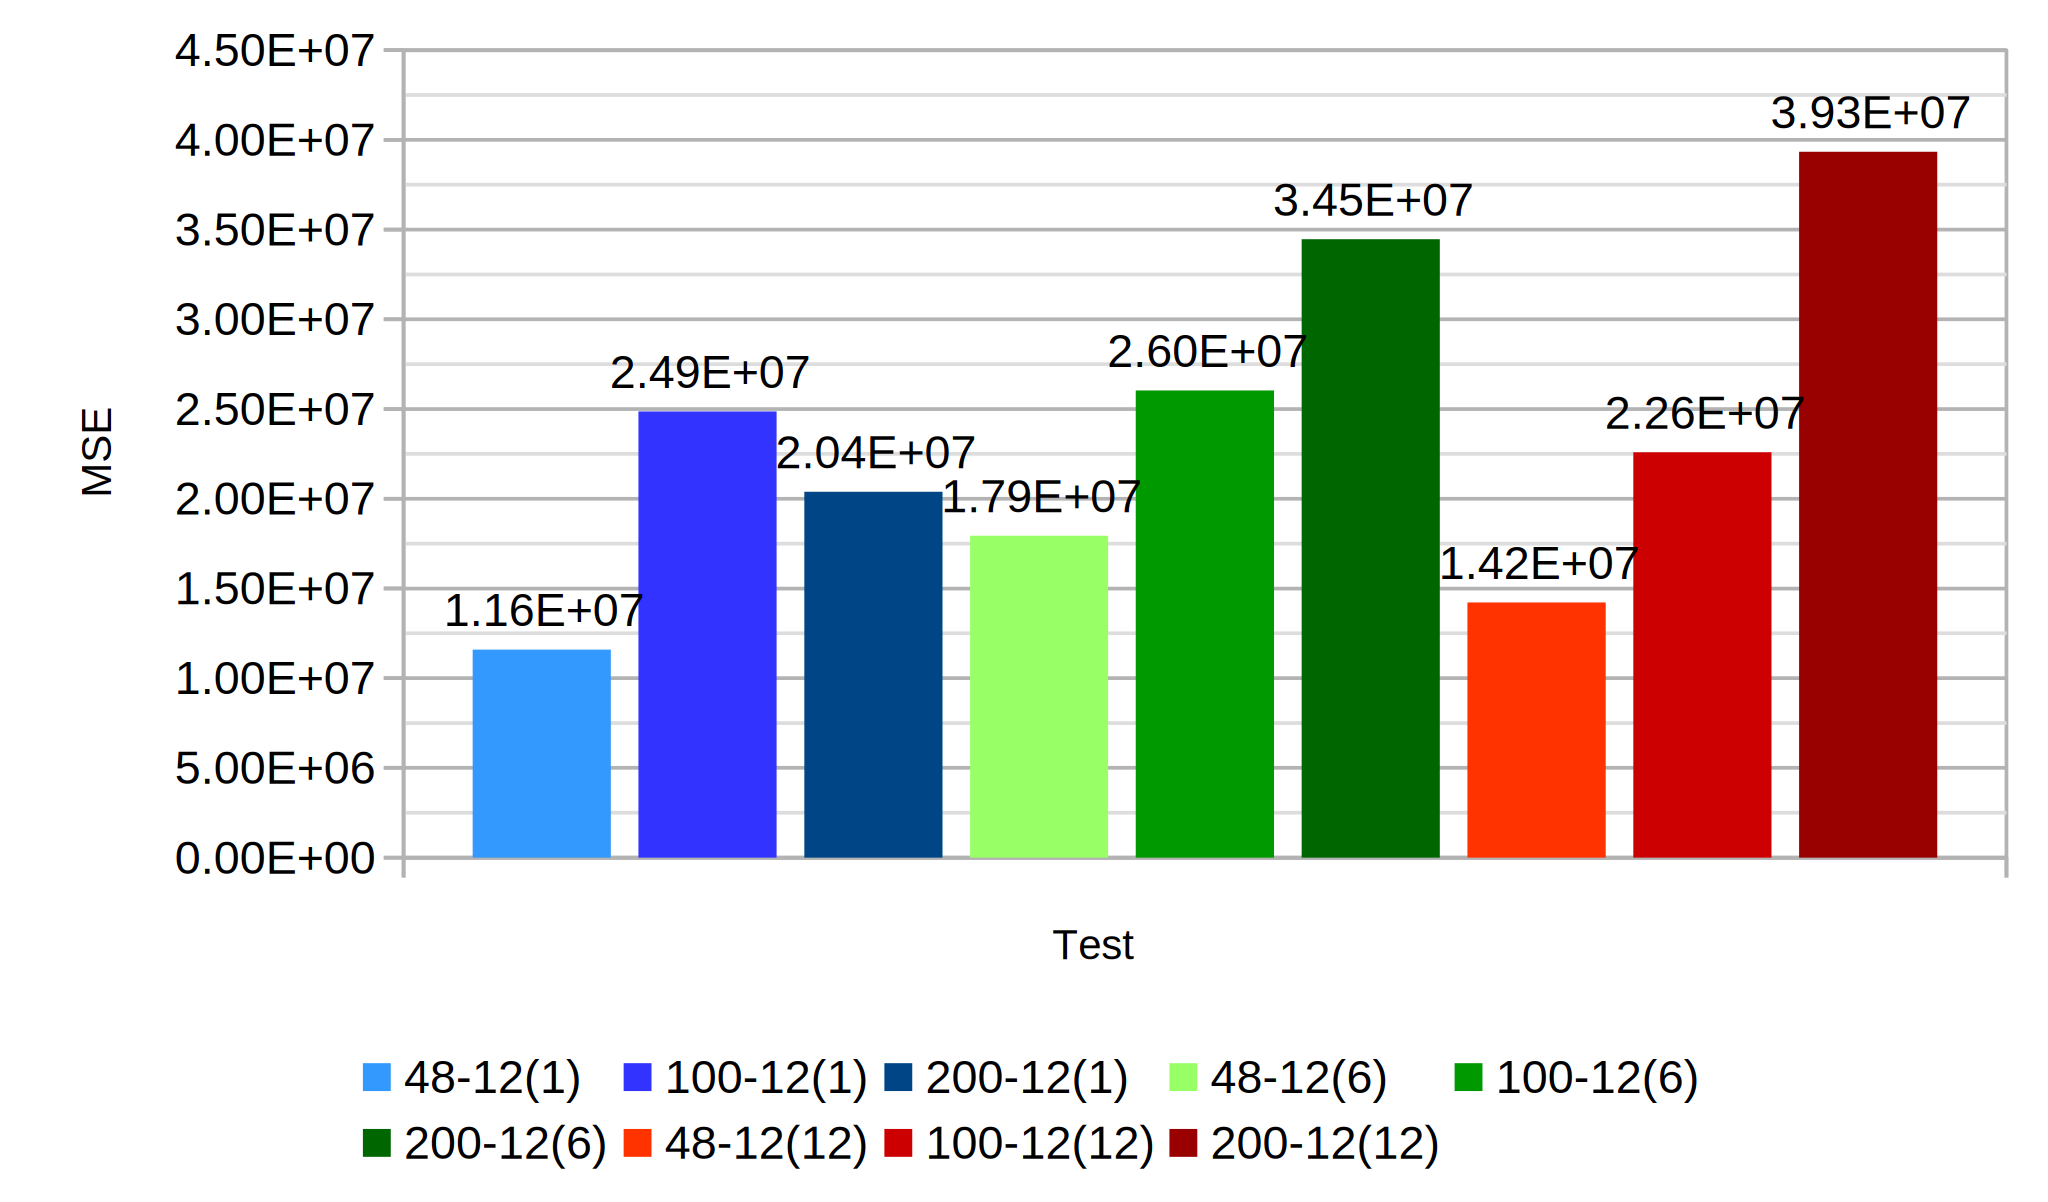
\includegraphics[angle=0]{img/src/results-simple-mse.pdf}}
                \caption{Test results for simple exponential smoothing. Average values of MSE for all tests samples.}
                \label{img:results-simple-mse}
            \end{center}
        \end{figure}

        %%%%%%%%
        \subsection{Double Exponential Smoothing} \label{sec:results-double}
        Complete raw tests results for double exponential smoothing are listed in Table \ref{appen:tab:double-results}.
        Chart \ref{img:results-double-pie} emphasizes that in 51\% tests Data Mining produces lower MSE than the
        equivalent R model. Five tests fall into the interval \interval[{1.1,1.2}] and one test has higher
        MSE than 20\%. Best result is for test case 100\,--\,12(12) where Data Mining produces lower MSE of 13\%.

        Averages of MSE ratios are depicted in Chart \ref{img:results-double-r}. Only three test cases have higher
        MSE than 1\% to maximum 6\%. The chart also shows that in average the
        lowest MSE ratios are for training set of length 48 observations. It meas that if results are compared to
        R in terms of training size R produces higher mean square error for larger training sets.

        \begin{figure}[H]
            \begin{center}
                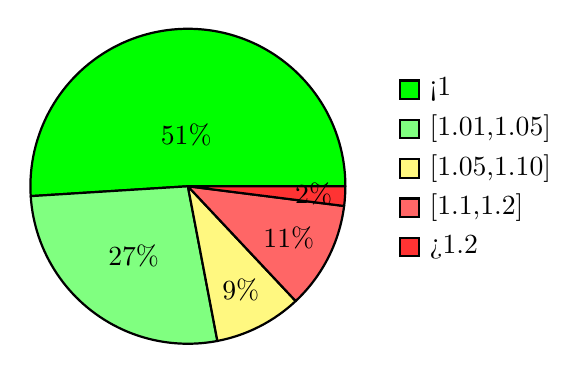
\begin{tikzpicture}
                    \pie[text=legend, radius=2, color={green!100 , green!50, yellow!50, red!60, red!80}]
                    {51/<1,
                    27/\interval[{1.01,1.05}],
                    9/\interval[{1.05,1.10}],
                    11/\interval[{1.1,1.2}],
                    2/>1.2}
                \end{tikzpicture}
                \caption{The proportion of Data Mining MSE to R MSE ratios split into intervals.}
                \label{img:results-double-pie}
            \end{center}
        \end{figure}

        \begin{figure}[H]
            \begin{center}
                \scalebox{0.65}[0.45]{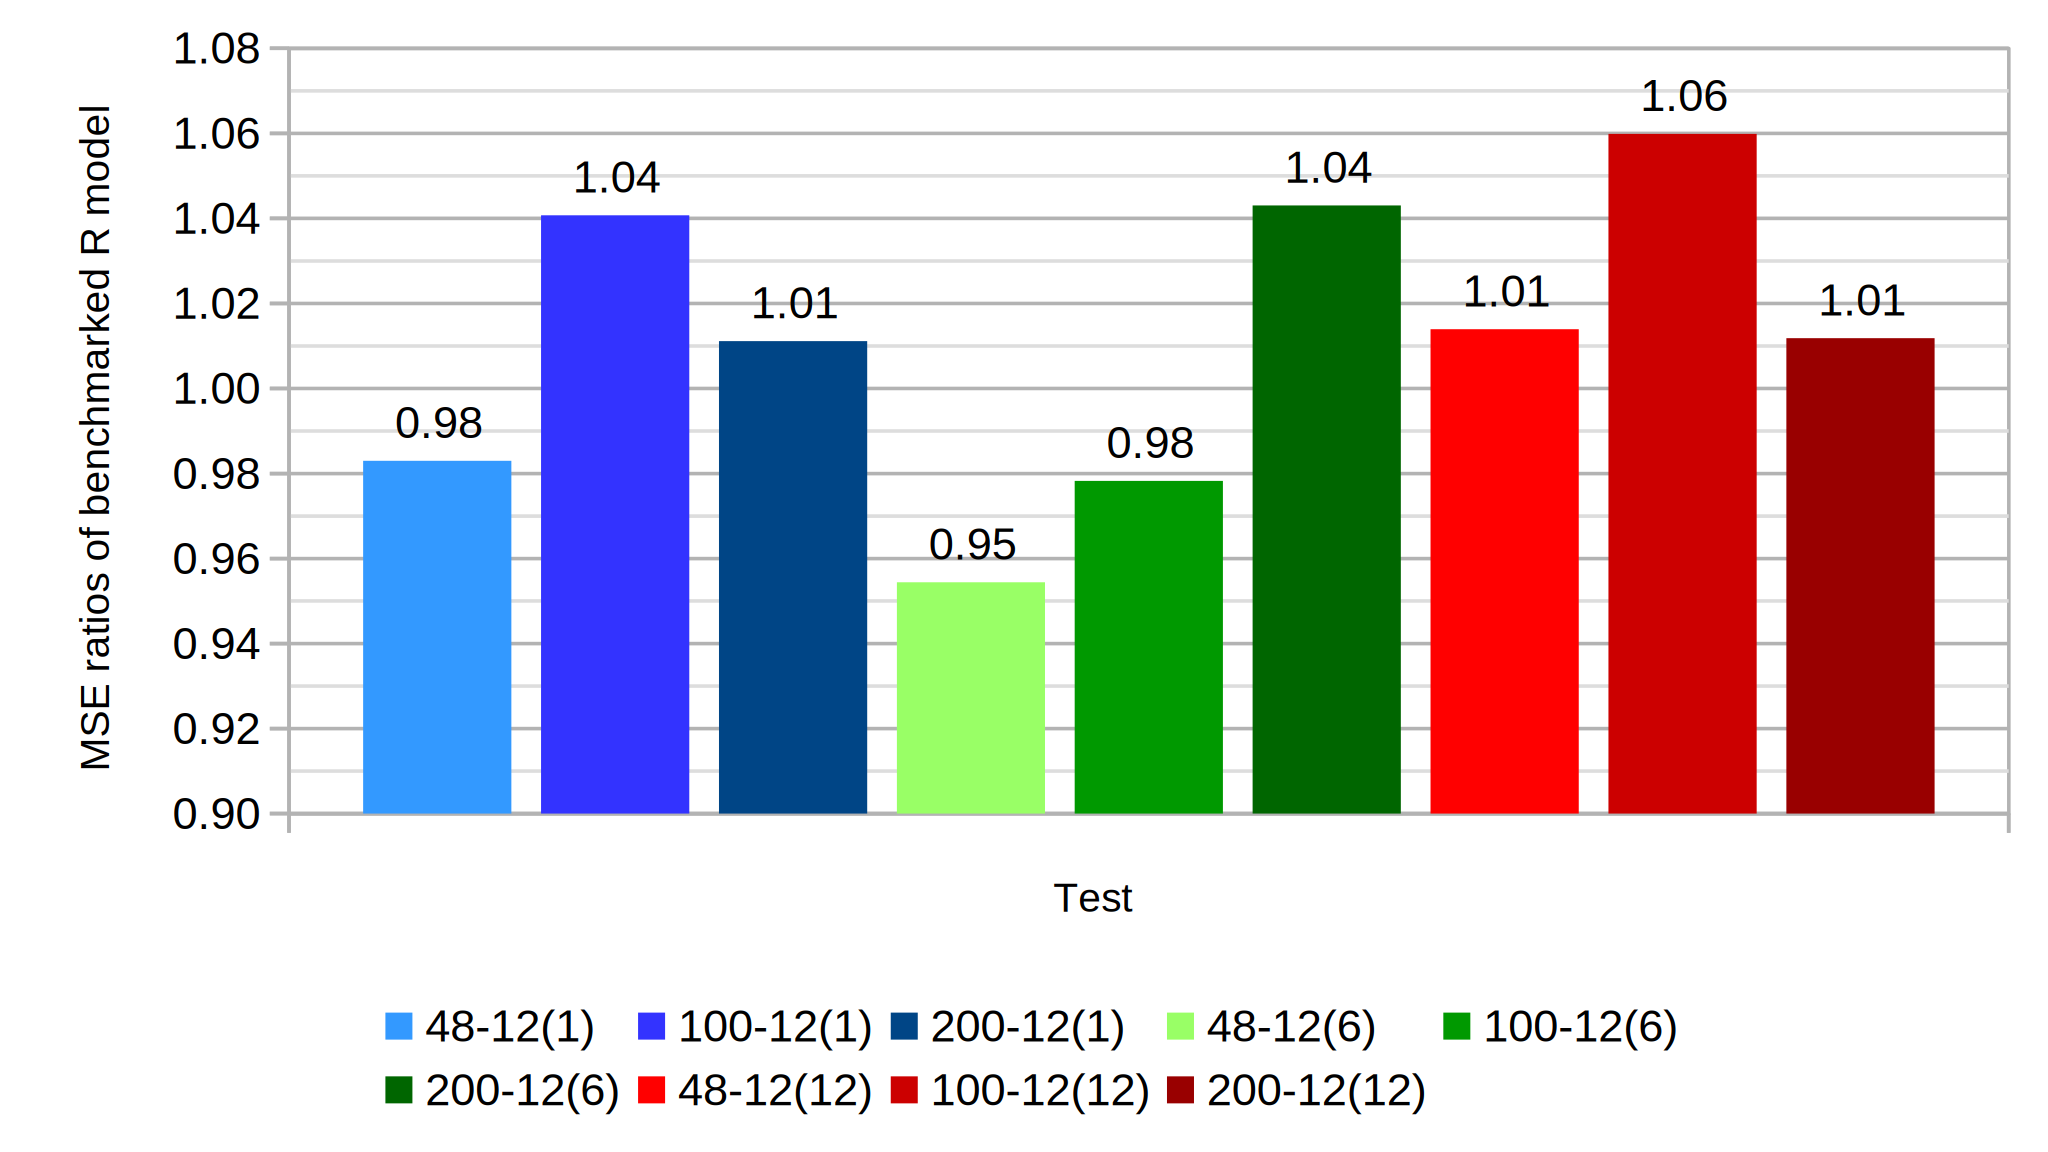
\includegraphics[angle=0]{img/src/results-double-r.pdf}}
                \caption{Test results for double exponential smoothing. Comparison to reference R model.}
                \label{img:results-double-r}
            \end{center}
        \end{figure}

        The last chart for double exponential smoothing is \ref{img:results-double-mse}.
        It shows that model similarly as simple exponential smoothing produces higher MSE for larger training sets.

        \begin{figure}[H]
            \begin{center}
                \scalebox{0.65}[0.45]{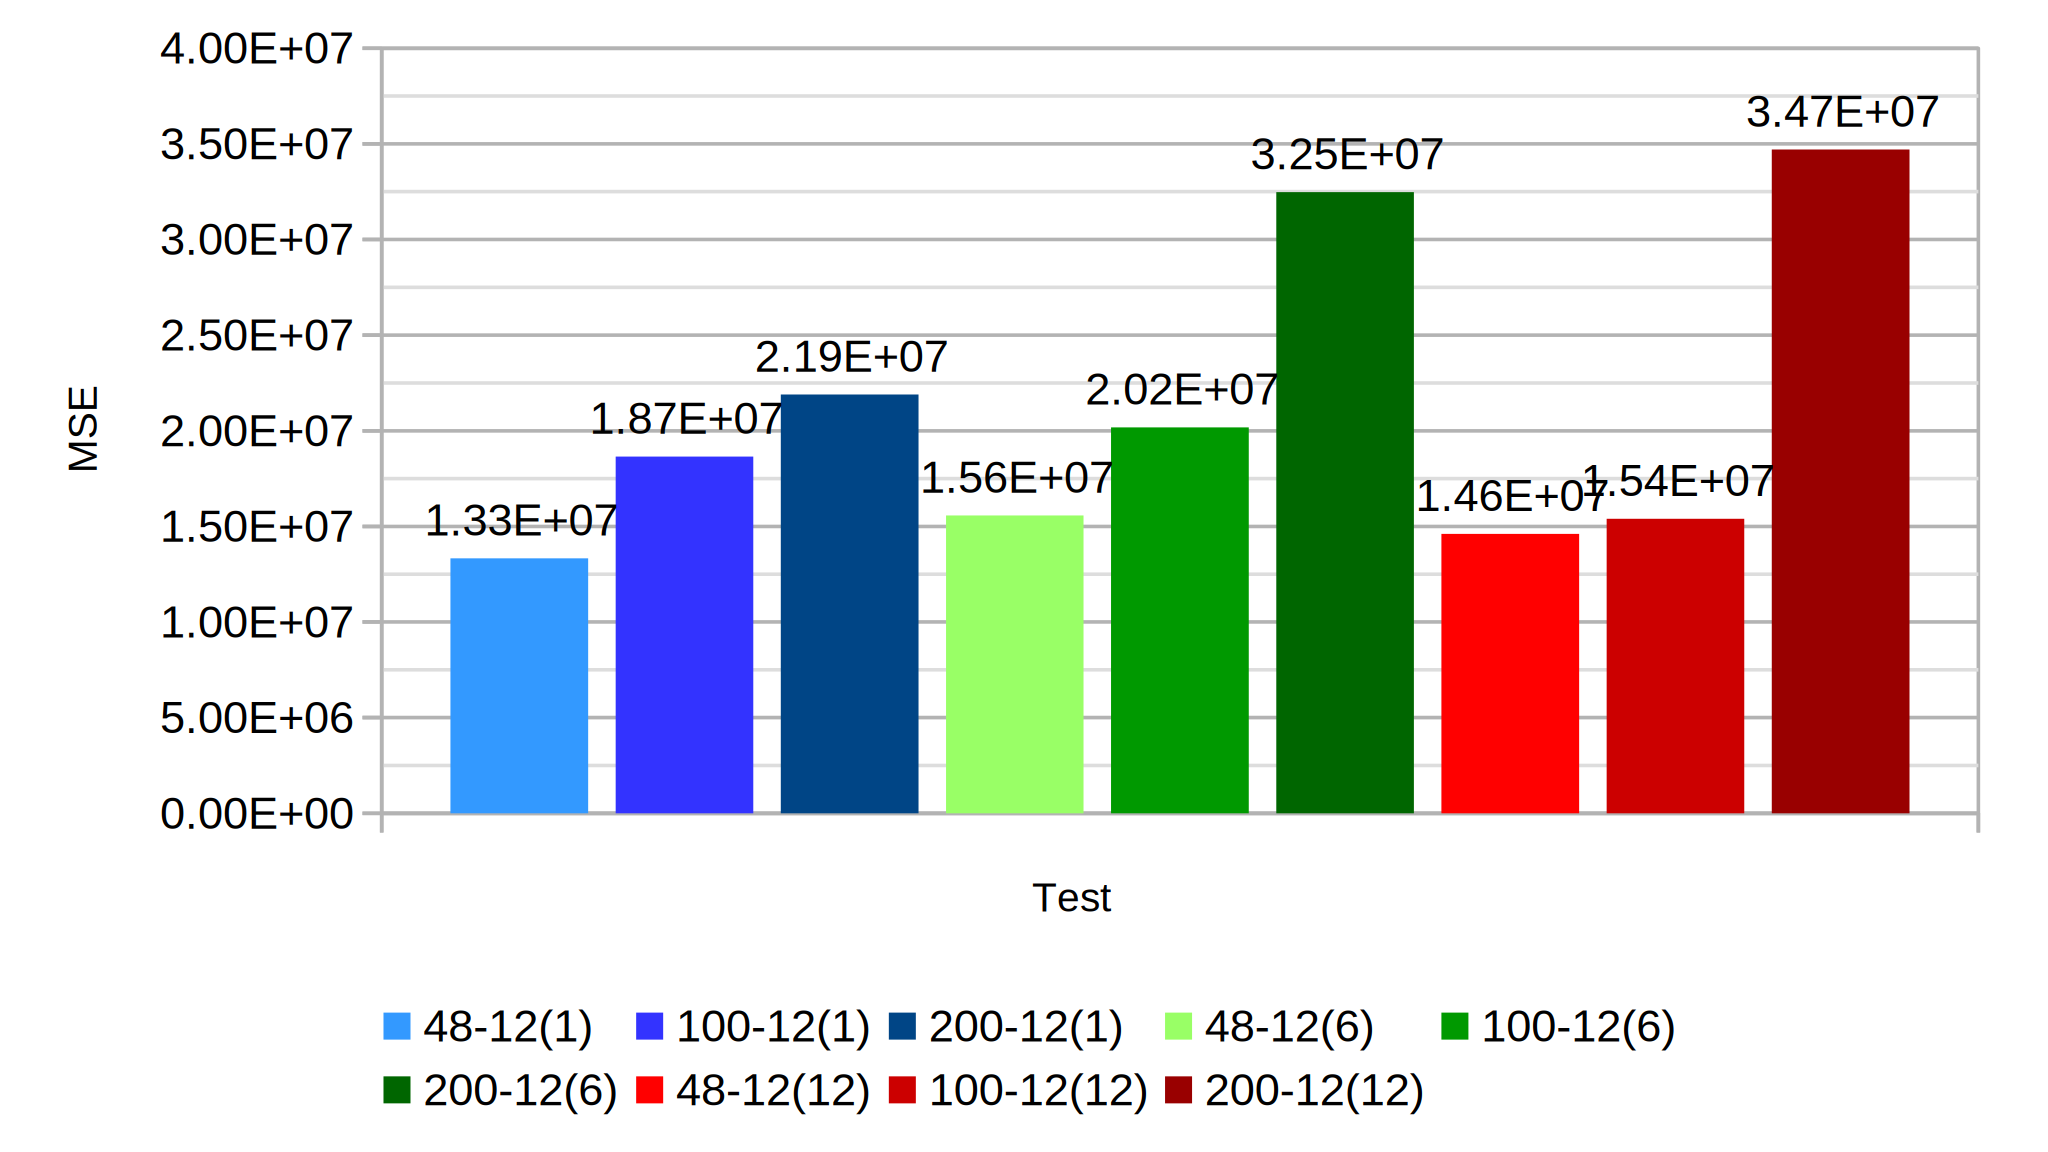
\includegraphics[angle=0]{img/src/results-double-mse.pdf}}
                \caption{Test results for double exponential smoothing. Average values of MSE for all tests samples.}
                \label{img:results-double-mse}
            \end{center}
        \end{figure}

        %%%%%%%%
        \subsection{Triple Exponential Smoothing} \label{sec:results-triple}
        Raw tests results for triple exponential smoothing are listed in Table \ref{appen:tab:triple-results}. In
        this case test cases can be run only on two data sets, because it does not make sense to fit seasonal
        model on non seasonal data. Therefore in total only eighteen tests were performed.

        During the testing it was observed that execution time of R script takes significantly more time than for other
        exponential smoothing models. On the other hand Data Mining implementation for triple exponential smoothing
        does not take more time compared to other exponential smoothing models. Table \ref{tab:datamining-perf} shows
        that R in average for one estimation takes 0.209 seconds which is for eighteen executions equals to 3.8 seconds.
        Whereas one estimation in Data Mining takes in average 0.023 seconds so time for eighteen estimation is 0.4
        seconds.

        Pie Chart \ref{img:results-triple-pie} shows that Data Mining triple exponential smoothing produces lower MSE
        in 67\% of all eighteen tests. It is better result than for simple or double exponential smoothing. However
        three tests produced MSE higher than 20\%. This could happen for example because R may use some better strategy
        for decomposing time series and setting seasonal indices.

        \begin{figure}[H]
            \begin{center}
                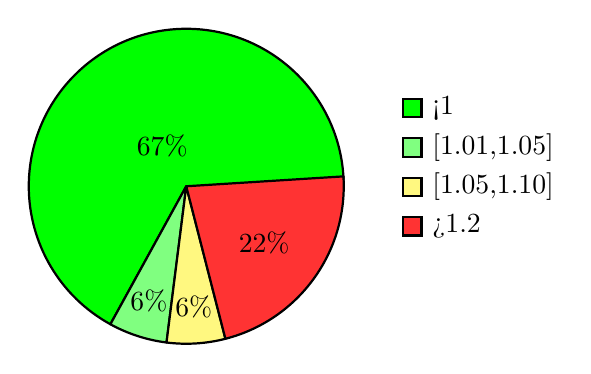
\begin{tikzpicture}
                    \pie[text=legend, radius=2, color={green!100 , green!50, yellow!50, red!80}]
                    {67/<1,
                    6/\interval[{1.01,1.05}],
                    6/\interval[{1.05,1.10}],
%                    11/ \interval[{1.1,1.2}],
                    22/>1.2}
                \end{tikzpicture}
                \caption{The proportion of Data Mining MSE to R MSE ratios split into intervals.}
                \label{img:results-triple-pie}
            \end{center}
        \end{figure}

        Averages of the MSE ratios are showed in Chart \ref{img:results-triple-r}. From the chart it can be seen that
        four out of nine tests produces higher MSE. R produces only 0.95 MSE in test case 200\,--\,12(12) on
        \texttt{sine} sample, but for smaller training sizes it produces 4.31 and 2.26 which is quite unstable result.
        Data Mining produces 4.07, 2.15 and 2.63 (training sets of size 50, 100 and 200). This causes significantly
        higher ratio for this test case.

        Overall results for averaged MSE ratios show that Data Mining performs better than R on smaller training sets.

        \begin{figure}[H]
            \begin{center}
                \scalebox{0.65}[0.44]{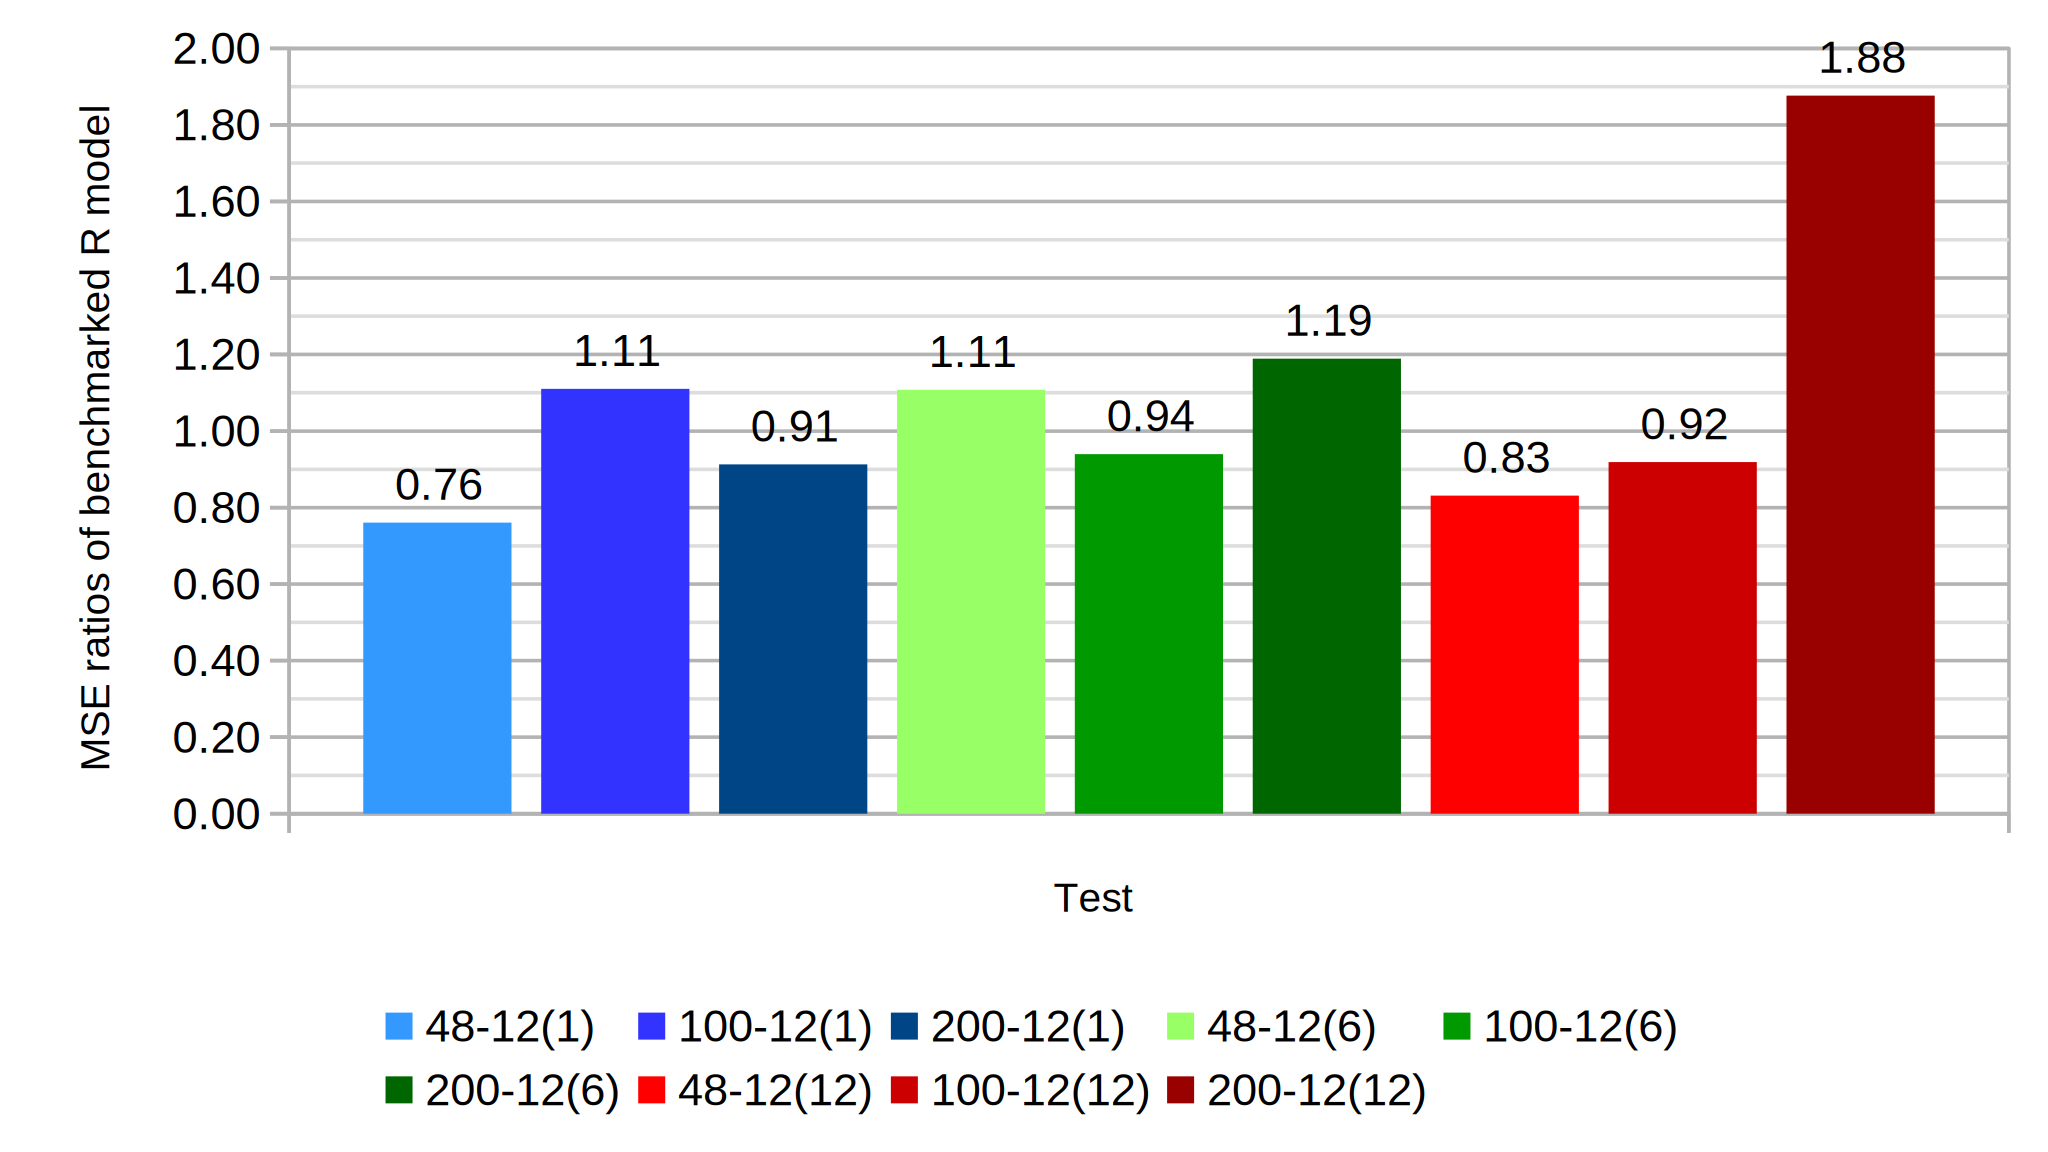
\includegraphics[angle=0]{img/src/results-triple-r.pdf}}
                \caption{Test results for triple exponential smoothing. Comparison to reference R model.}
                \label{img:results-triple-r}
            \end{center}
        \end{figure}

        Chart \ref{img:results-triple-mse} emphasize that larger training size does improve forecasting accuracy. It is
        the same result as for other models.

        \begin{figure}[H]
            \begin{center}
                \scalebox{0.65}[0.44]{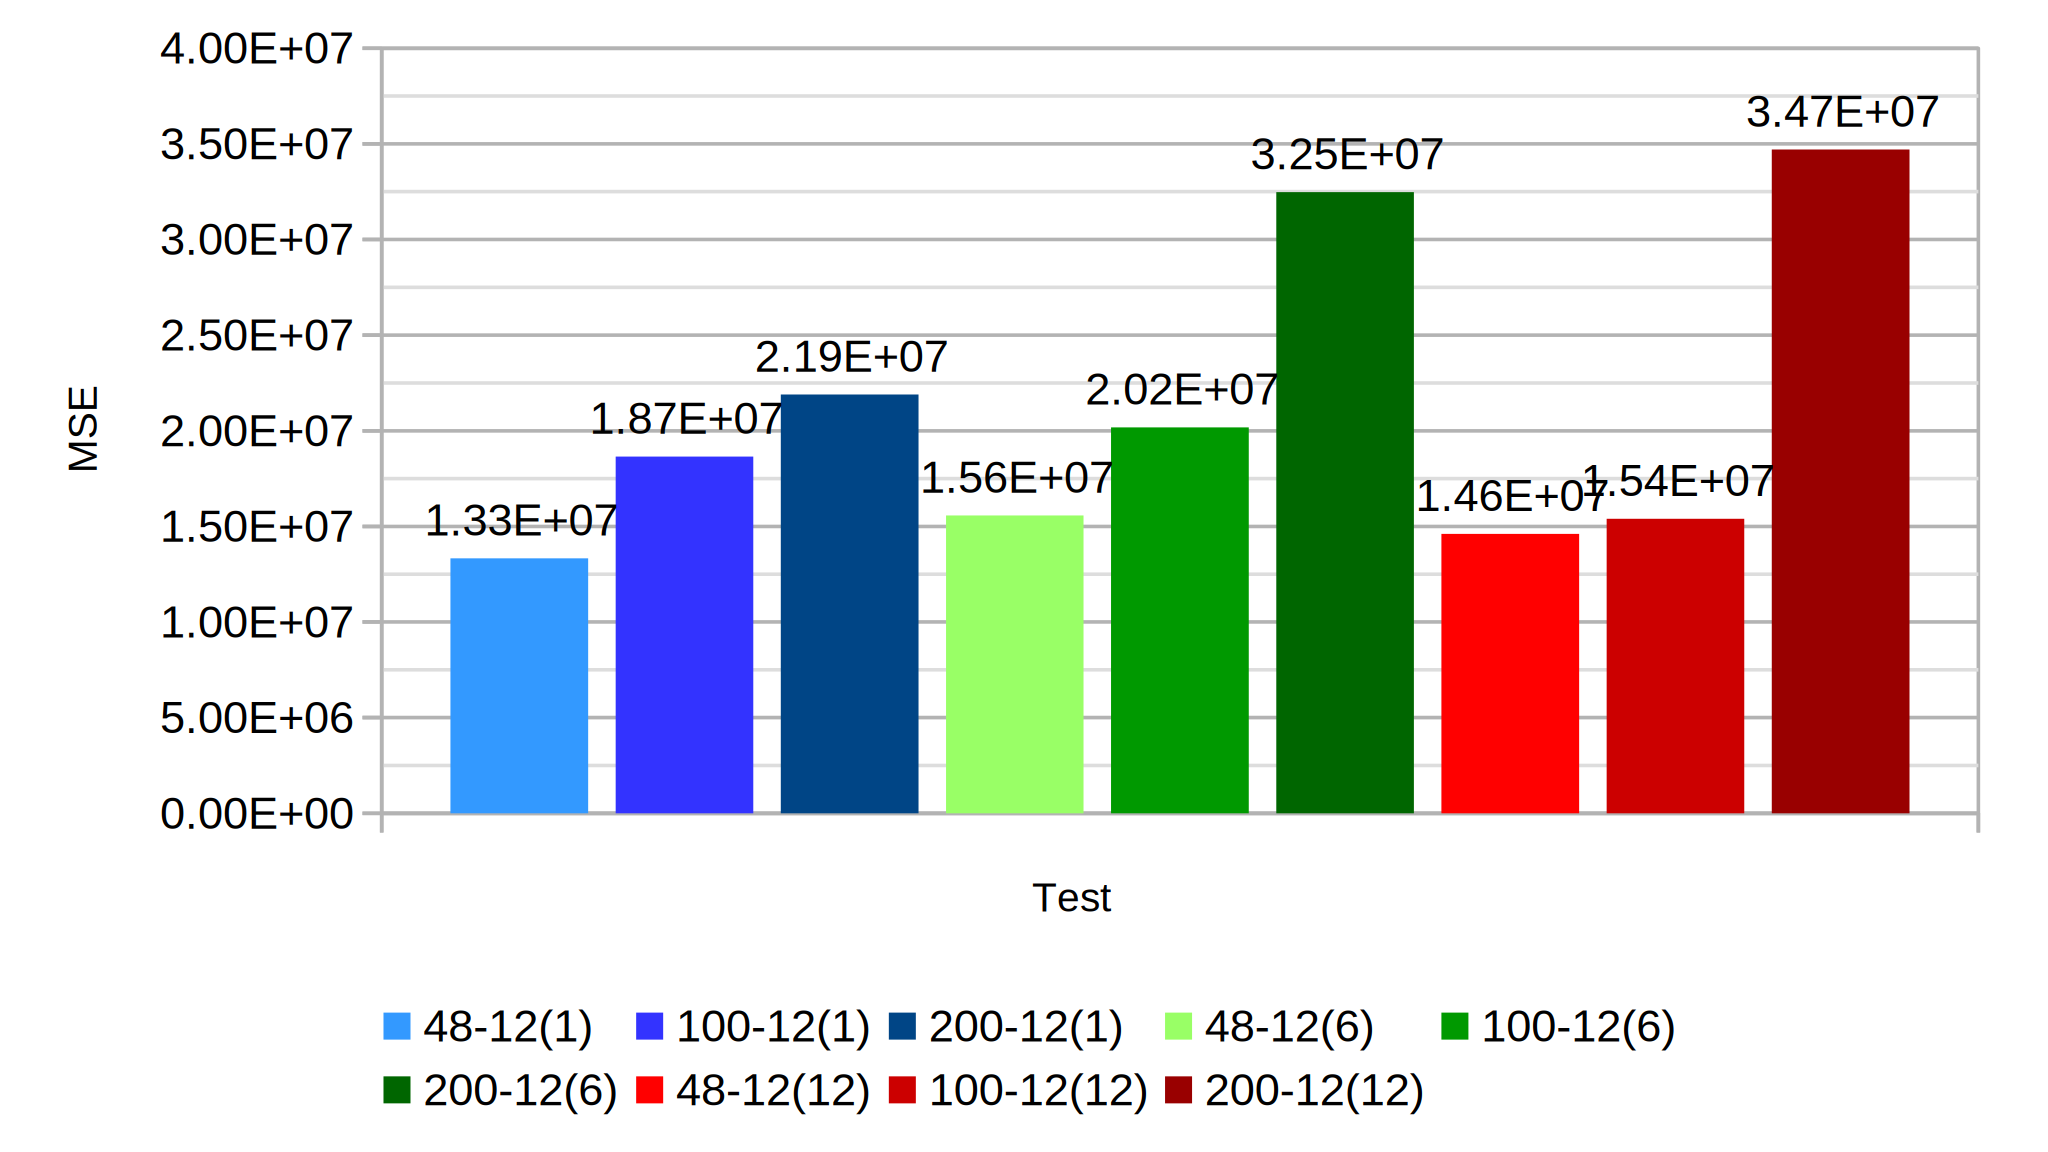
\includegraphics[angle=0]{img/src/results-double-mse.pdf}}
                \caption{Test results for triple exponential smoothing. Average values of MSE for all tests samples.}
                \label{img:results-triple-mse}
            \end{center}
        \end{figure}

        %%%%%%%%
        \subsection{Overall Results} \label{sec:overall}
        This section contains aggregated results for simple, double and triple exponential smoothing models.

        Chart \ref{img:results-overall-r} highlights that only in four tests Data Mining models in average produce
        higher MSE than alternative R models. Test case 200\,--\,12(12) shows the worst result which is 28\%
        higher than benchmarked R model. This was discussed in Section \ref{sec:results-triple}.

        Average for all test cases is equal to 2\%. In other words Data Mining models in average produced mean
        squared error higher than 2\% compared to R models. Therefore Data Mining model's prediction capabilities
        can be considered as R alternatives.

        \begin{figure}[H]
            \begin{center}
                \scalebox{0.65}[0.45]{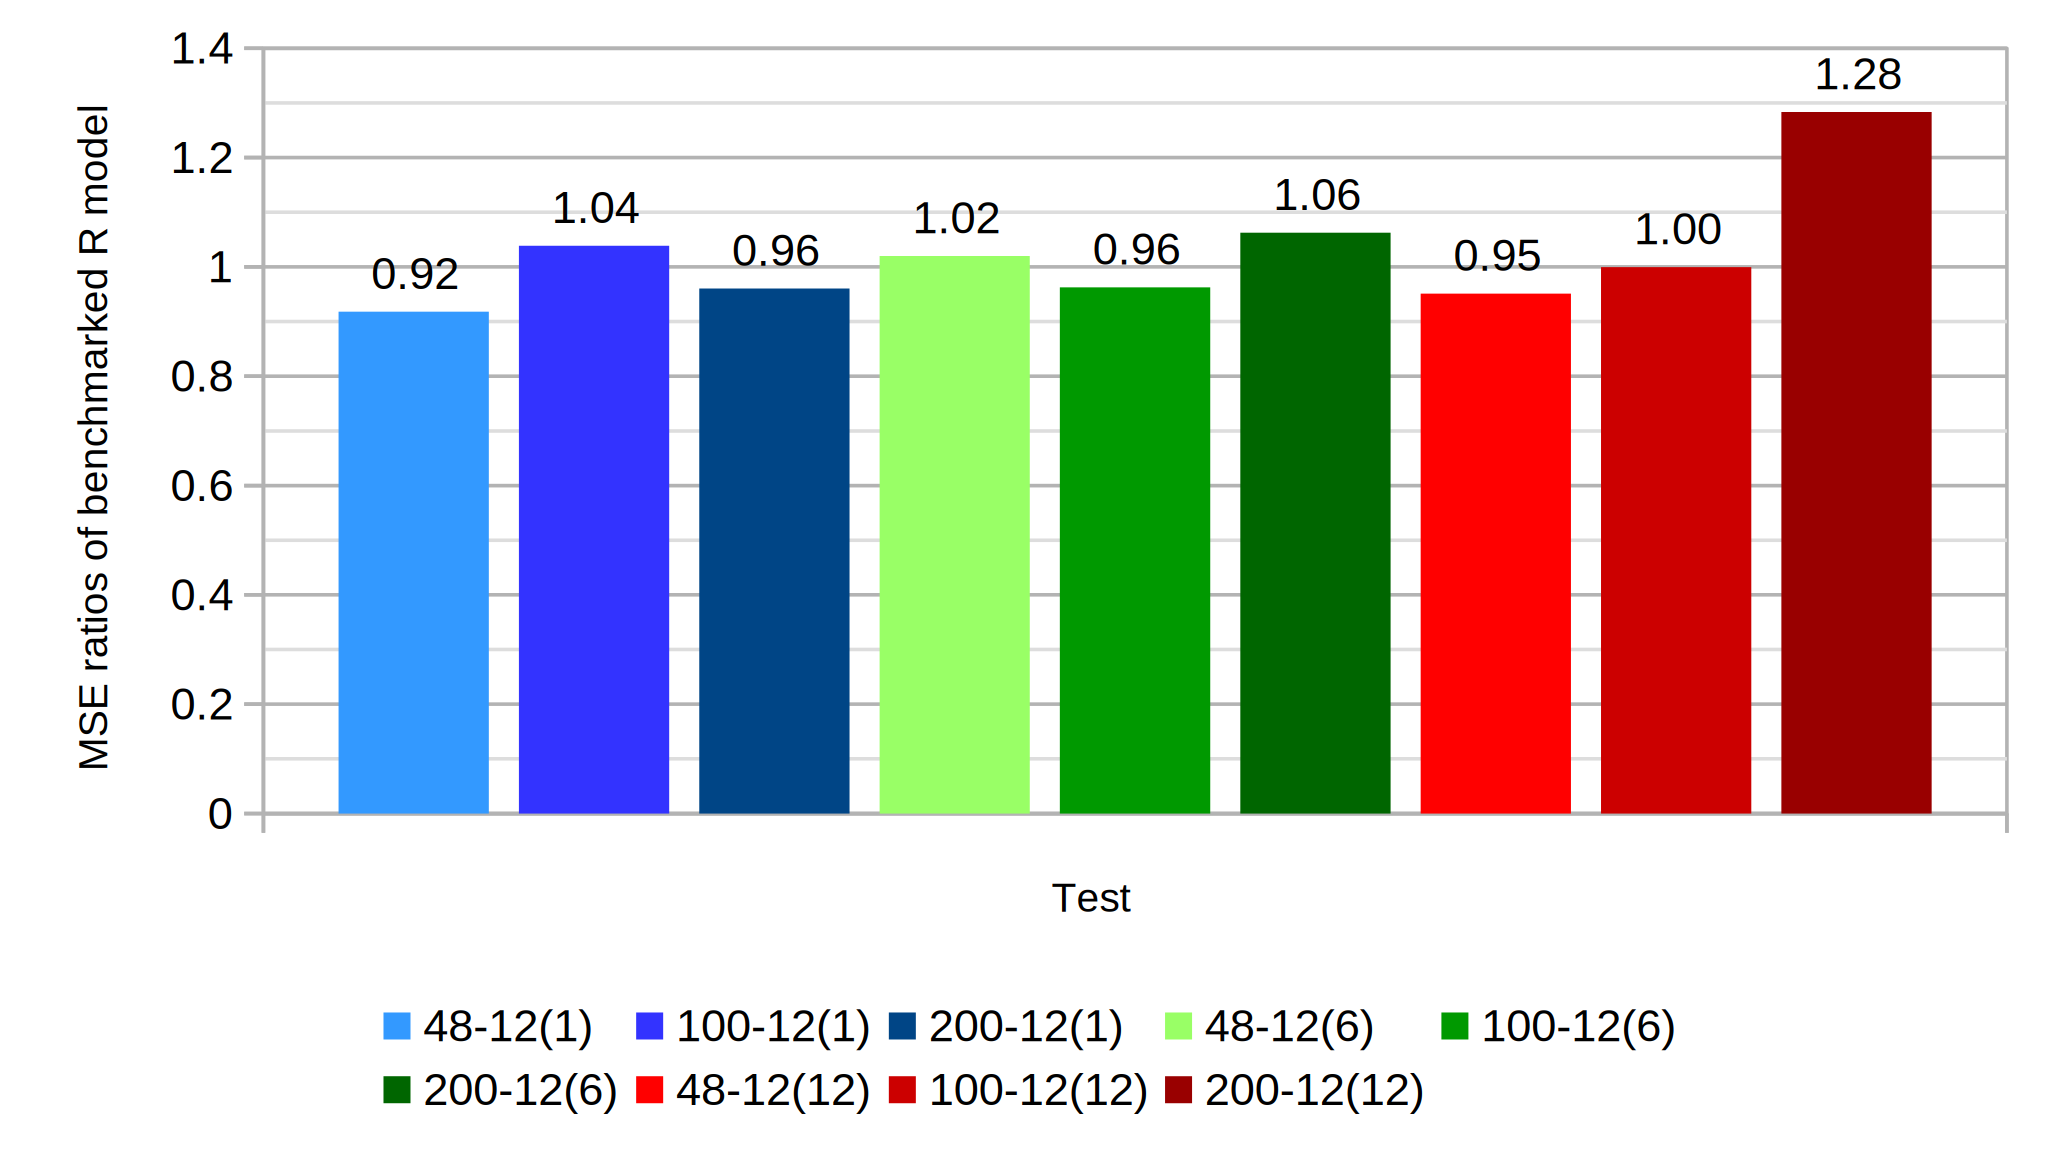
\includegraphics[angle=0]{img/src/results-overall-r.pdf}}
                \caption{Aggregated test results for all models. Comparison to reference R model.}
                \label{img:results-overall-r}
            \end{center}
        \end{figure}

        Aggregated results for Data Mining mean squared errors are depicted in Chart \ref{img:results-overall-mse}. The
        results are similar to the results discussed for each model. It shows that longer training set does not
        improve forecasting accuracy. Further research could identify ideal size of training set. These tests
        proved that longer training size does not imply better forecasts.

        \begin{figure}[H]
            \begin{center}
                \scalebox{0.65}[0.45]{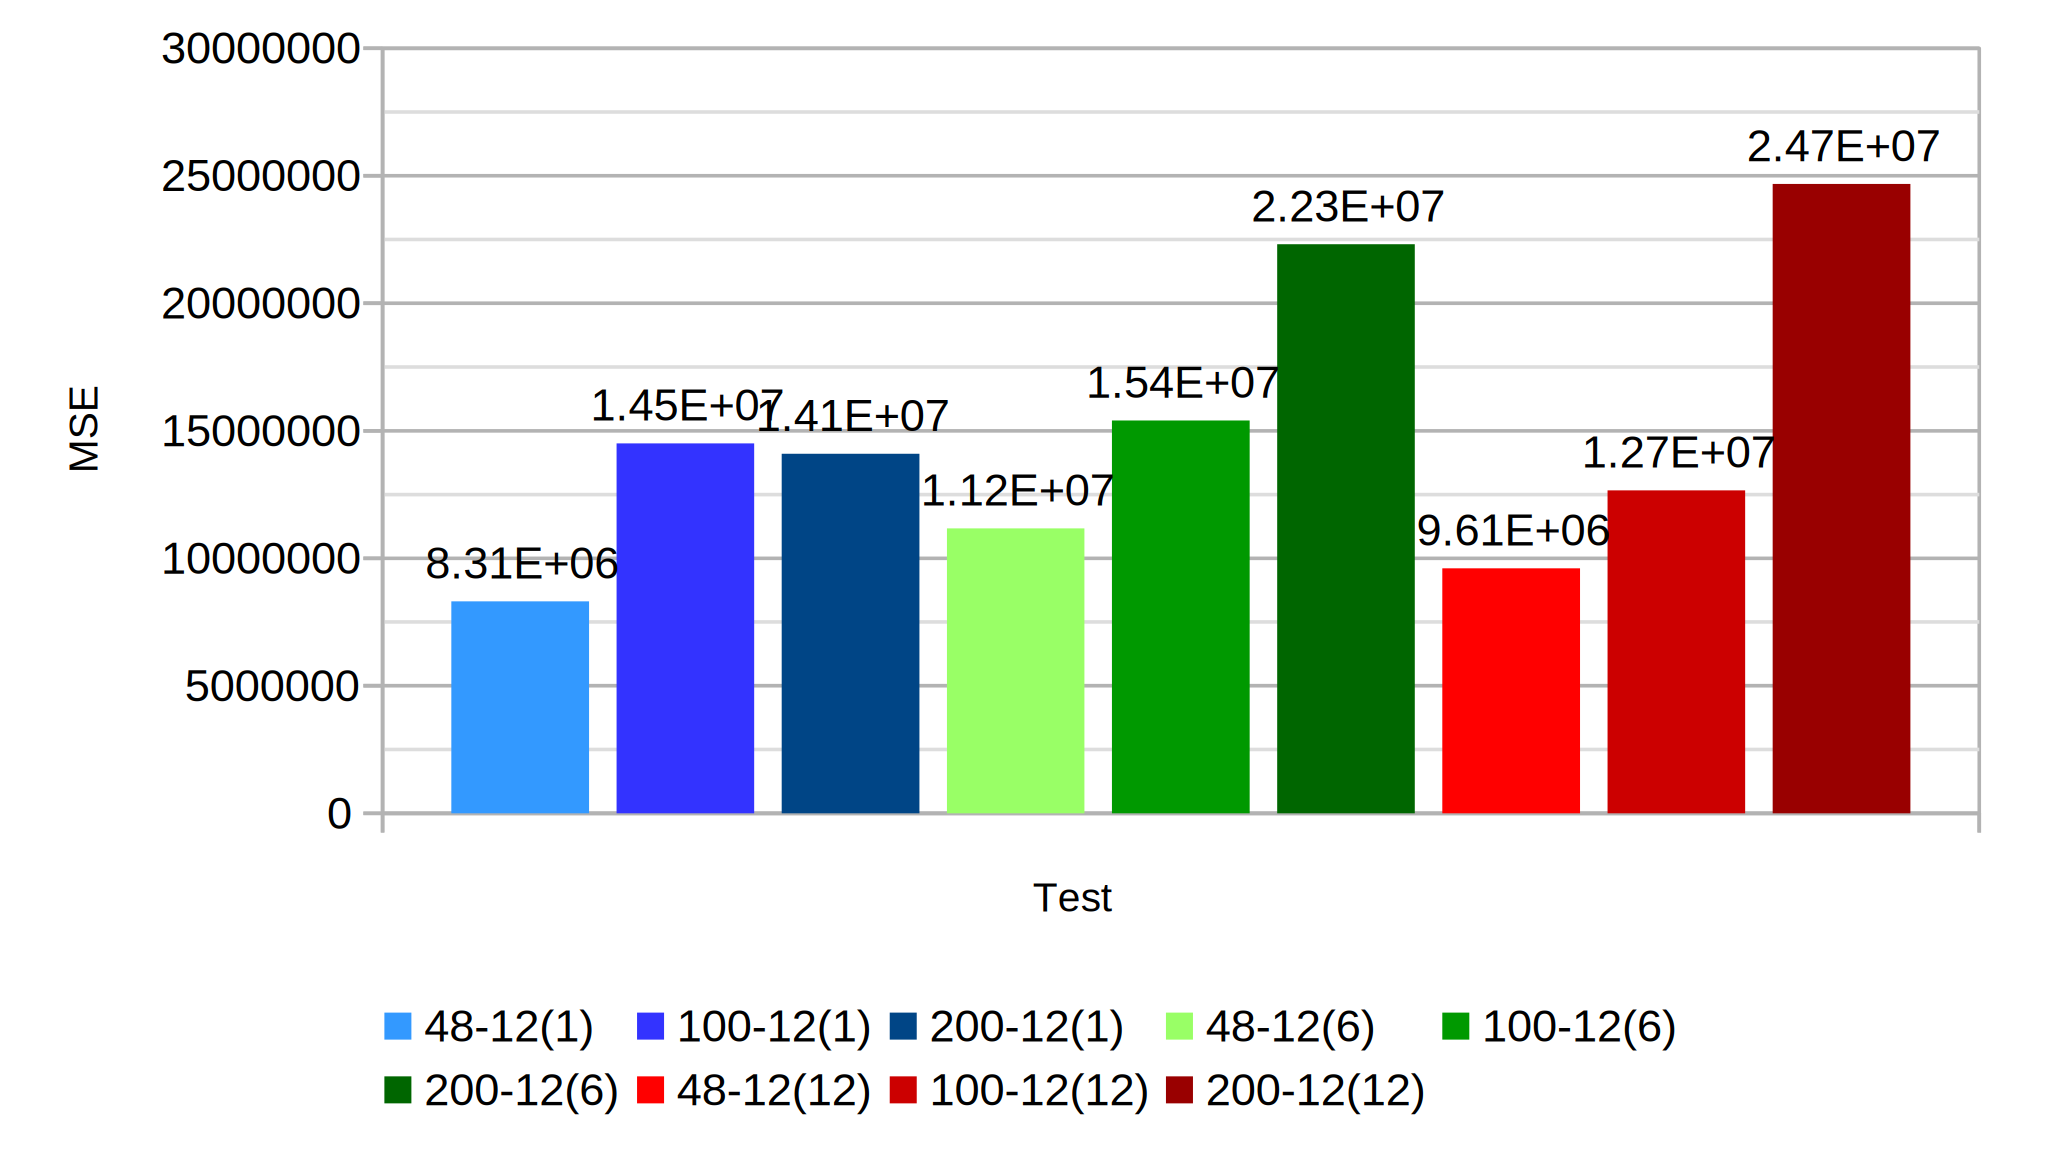
\includegraphics[angle=0]{img/src/results-overall-mse.pdf}}
                \caption{Aggregated test results for all models. Average values of MSE for all tests samples.}
                \label{img:results-overall-mse}
            \end{center}
        \end{figure}

%%%%%%%%%%%%%%%%%%%%%%%%%%%%%%%%%%%%%%%%%%%%%%%%%%%%%%%%%%%%%%%%%%%
\chapter{Conclusion} \label{chap:conclusion}
The goal of the master's thesis is to develop independent module in Java language for providing alert prediction
capabilities for open source project Hawkular.

Implementation part is split into multiple artifacts with dedicated functionality. The most important module
focuses on time series modelling. It contains simple, double and triple exponential smoothing models which
use non-linear optimization algorithm for finding the best parameters with goal of minimizing prediction error.
The library also contains several time series utility classes and statistical tests for time series analysis.

Data Mining prediction engine autonomously selects the best time series model for underlying time series. Most
importantly, it is capable of dealing with concept drift problem. So there is no need of any analytical configuration
in production.

The last chapter benchmarks forecasting accuracy of the implemented models. It is shown that forecasts produced by
implemented models are in some cases more accurate that forecast from package \texttt{forecast} from R language and
in average Data Mining models can be compared to R models. In terms of execution time performance Data Mining
models are much efficient.

During the development of the module, Hawkular was still in development phase, therefore it was not
possible to gather real data from production environment. This would help with tunning models for specific metrics
for example Java heap usage.

The module was successfully integrated into Hawkular and predictive charts of the metrics are located in Metric explorer
tab.

Future work on this module should analyze data from production servers and if necessary change the properties of
optimizers in order to get more accurate predictions. Analysis could also contain evaluation if damped trend should be
added to the implemented models.

As it is open source project, it would be great to attract more people into development and continue with adding new
models and features for time series analysis, because there is no widely used and maintained library for this purpose
in Java.


\makeatletter\thesis@blocks@clear\makeatother
\phantomsection %% Print the index and insert it into the
\addcontentsline{toc}{chapter}{\indexname} %% table of contents.

%\bibliographystyle{czechiso} % sets plain bibliography style
\bibliographystyle{czplain}
\bibliography{bibliography}     % BibTeX database file

\appendix %% Start the appendices.
\chapter{Diagrams}
    \begin{figure}[H]
        \begin{center}
            % original from idea
            %\scalebox{0.34}[0.475]{\includegraphics{img/src/maven-deps-tree.pdf}}
            \scalebox{0.6}{\includegraphics{img/src/maven-deps-tree.pdf}}
            \caption{Dependency tree of maven artifacts.}
            \label{appen:maven-deps}
        \end{center}
    \end{figure}

    \begin{figure}[H]
        \begin{center}
            \scalebox{0.35}[0.21]{\includegraphics[angle=90]{img/src/class-diagram.pdf}}
            \caption{Partial class diagram of \texttt{datamining-forecast} and \texttt{datamining-api}.}
            \label{appen:class-diagram}
        \end{center}
    \end{figure}

\chapter{Predictive Charts}
    \begin{figure}[H]
        \begin{center}
            \scalebox{0.6}[0.443]{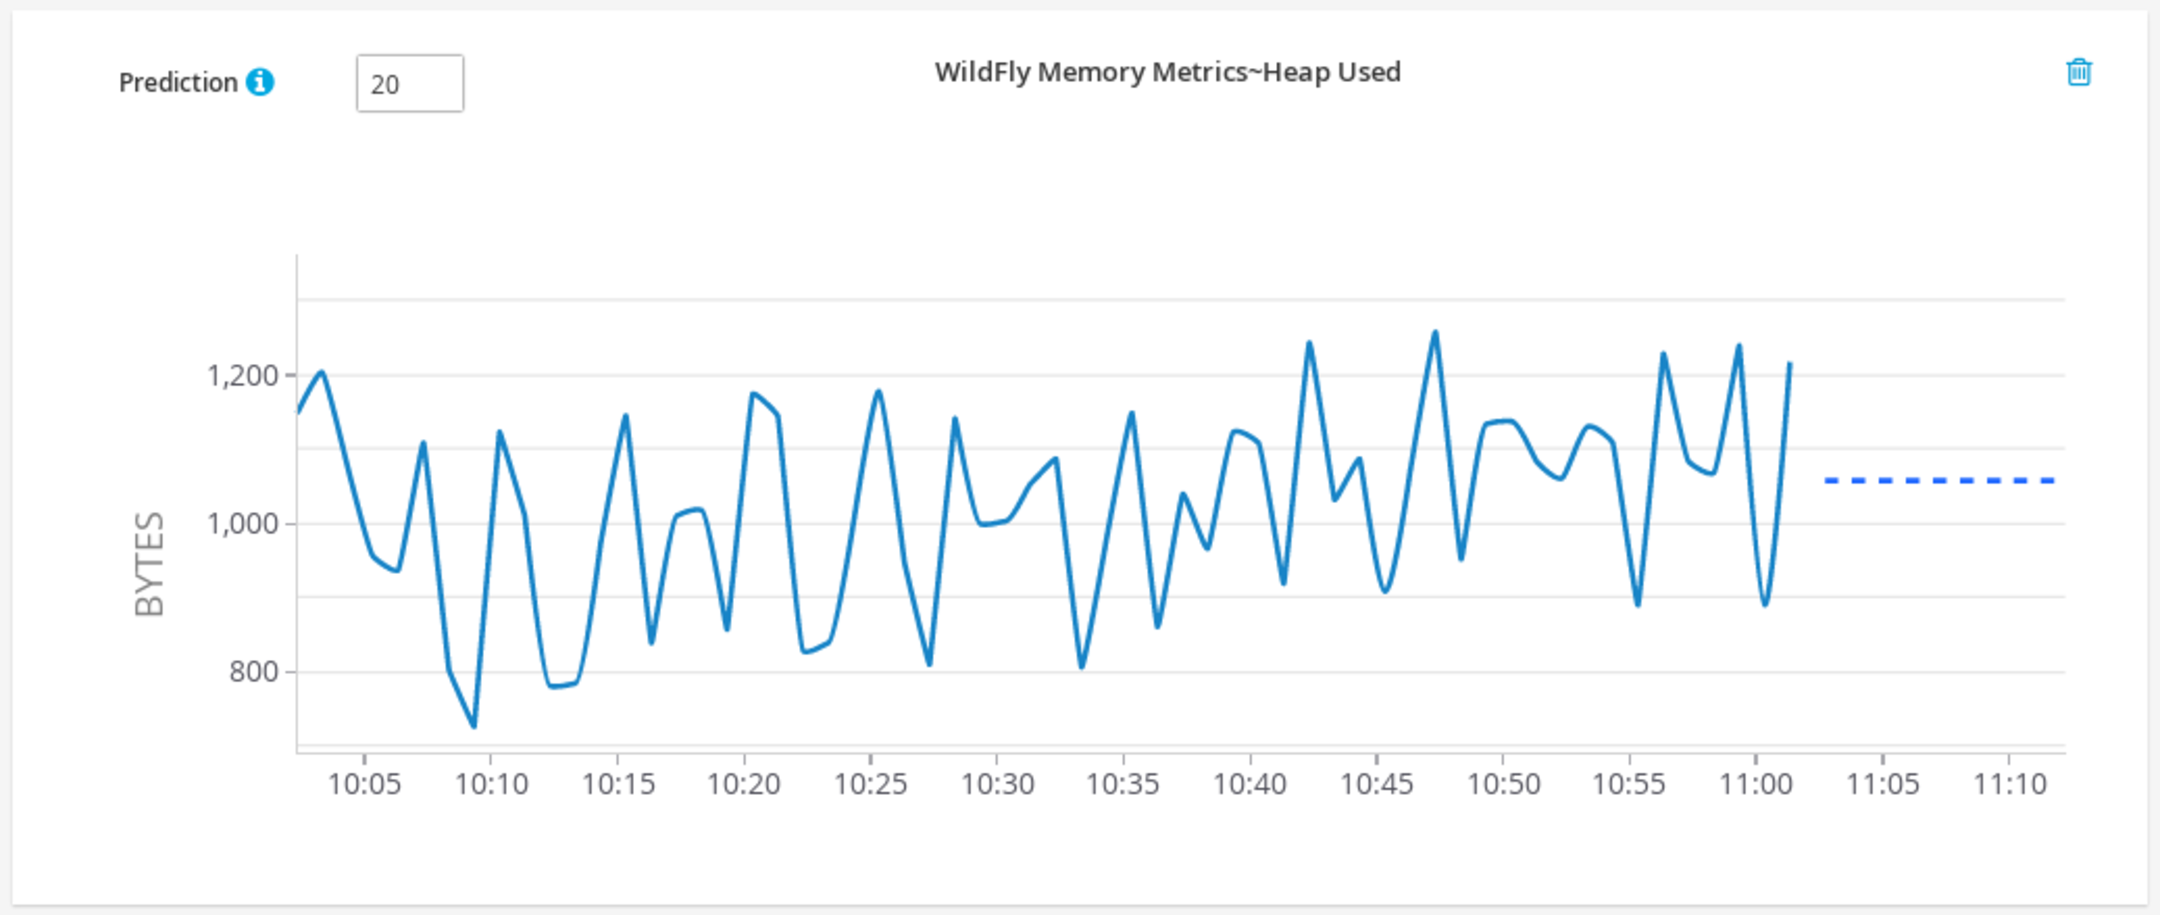
\includegraphics[angle=90]{img/hawkular-simple.pdf}}
            \caption{Predictive chart for simple exponential smoothing.}
            \label{appen:hawkular-simple}
        \end{center}
    \end{figure}
    \begin{figure}[H]
        \begin{center}
            \scalebox{0.6}[0.5]{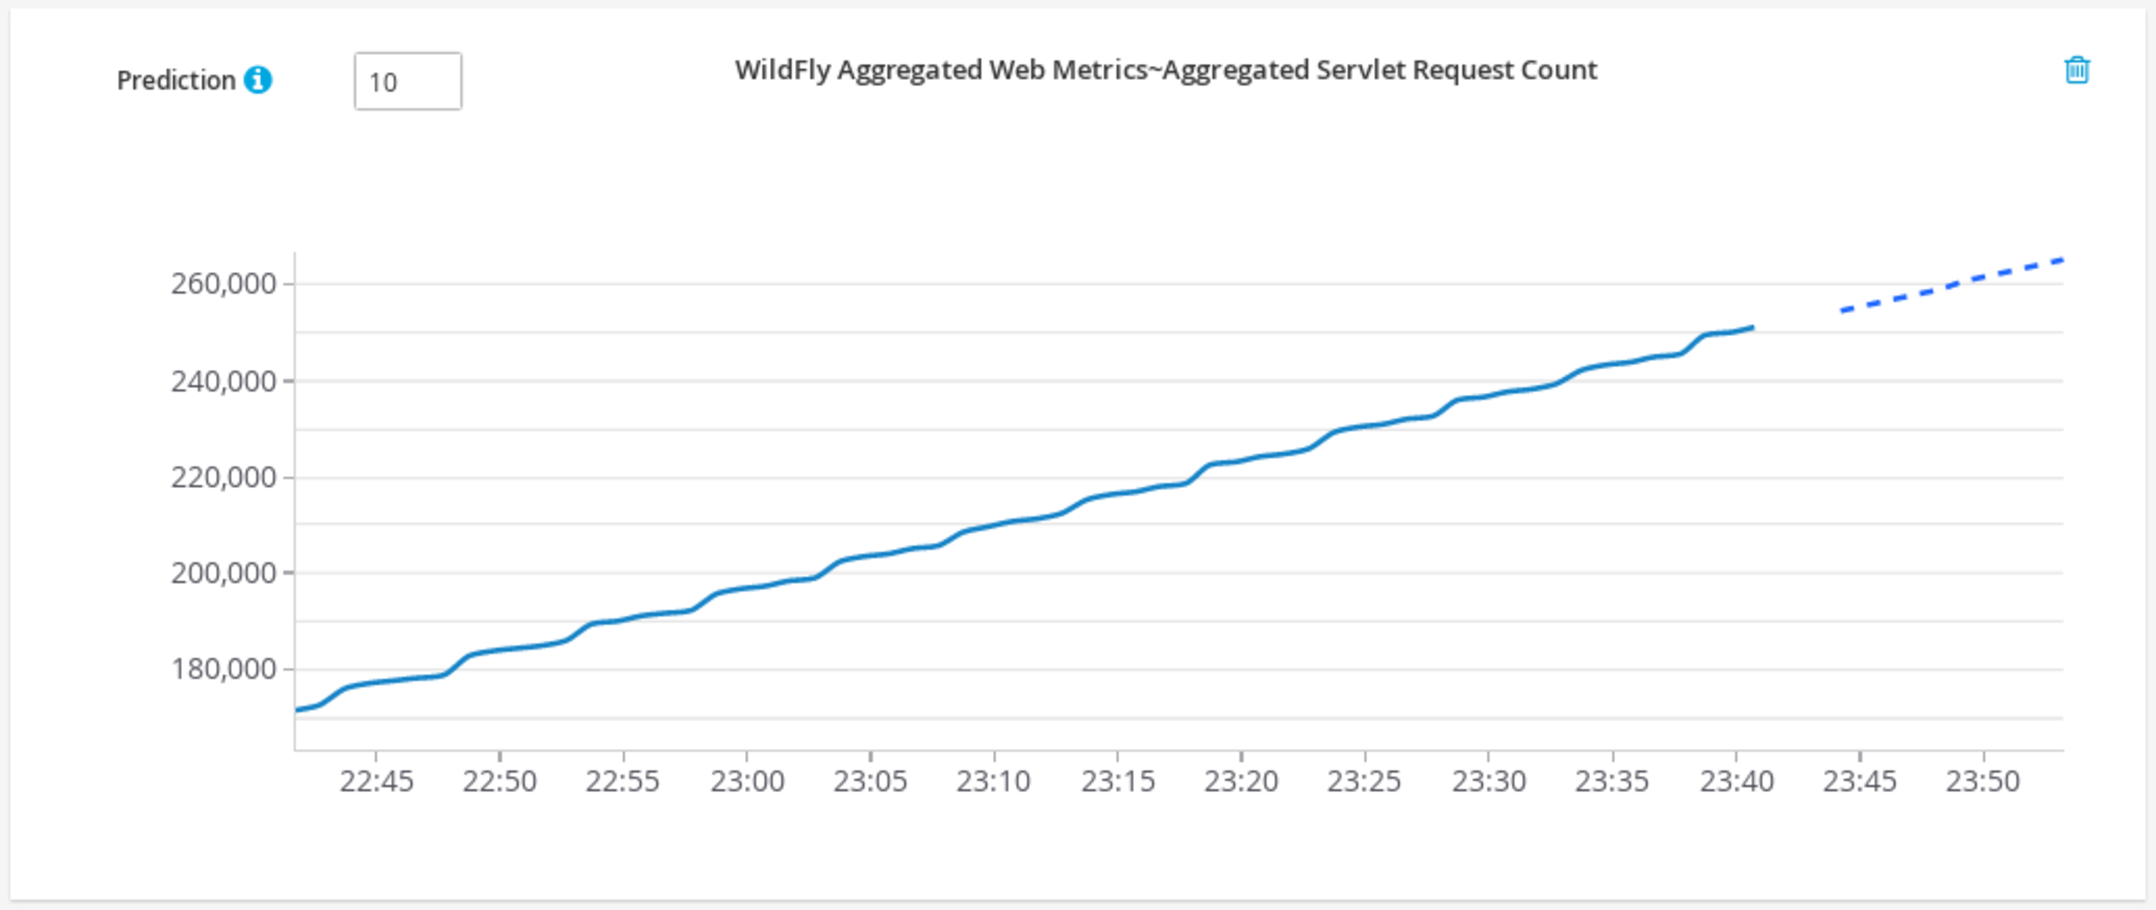
\includegraphics[angle=90]{img/hawkular-double.pdf}}
            \caption{Predictive chart for double exponential smoothing.}
            \label{appen:hawkular-double}
        \end{center}
    \end{figure}
    \begin{figure}[H]
        \begin{center}
            \scalebox{0.6}[0.5]{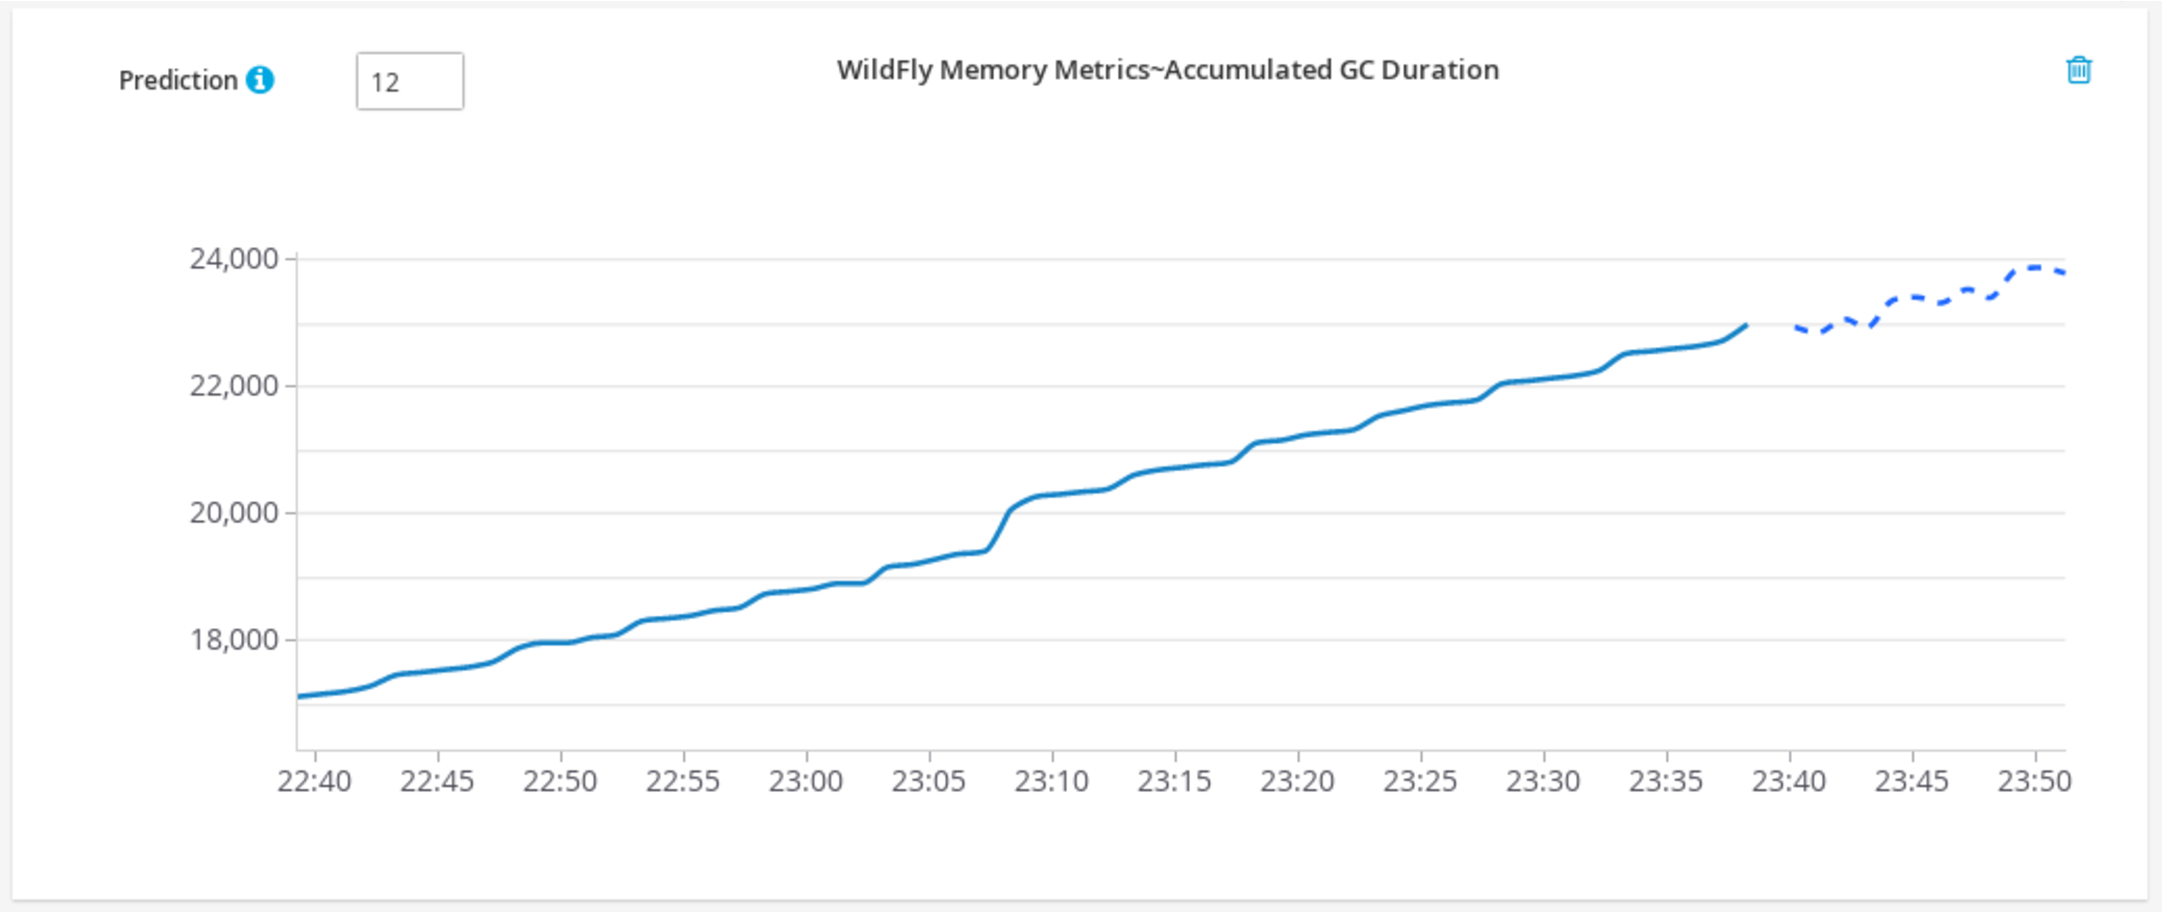
\includegraphics[angle=90]{img/hawkular-triple.pdf}}
            \caption{Predictive chart for triple exponential smoothing.}
            \label{appen:hawkular-triple}
        \end{center}
    \end{figure}

\chapter{Testing Time Series Samples} \label{appen:testing-samples}
    \begin{figure}[H]
        \begin{center}
            \scalebox{0.22}[0.62]{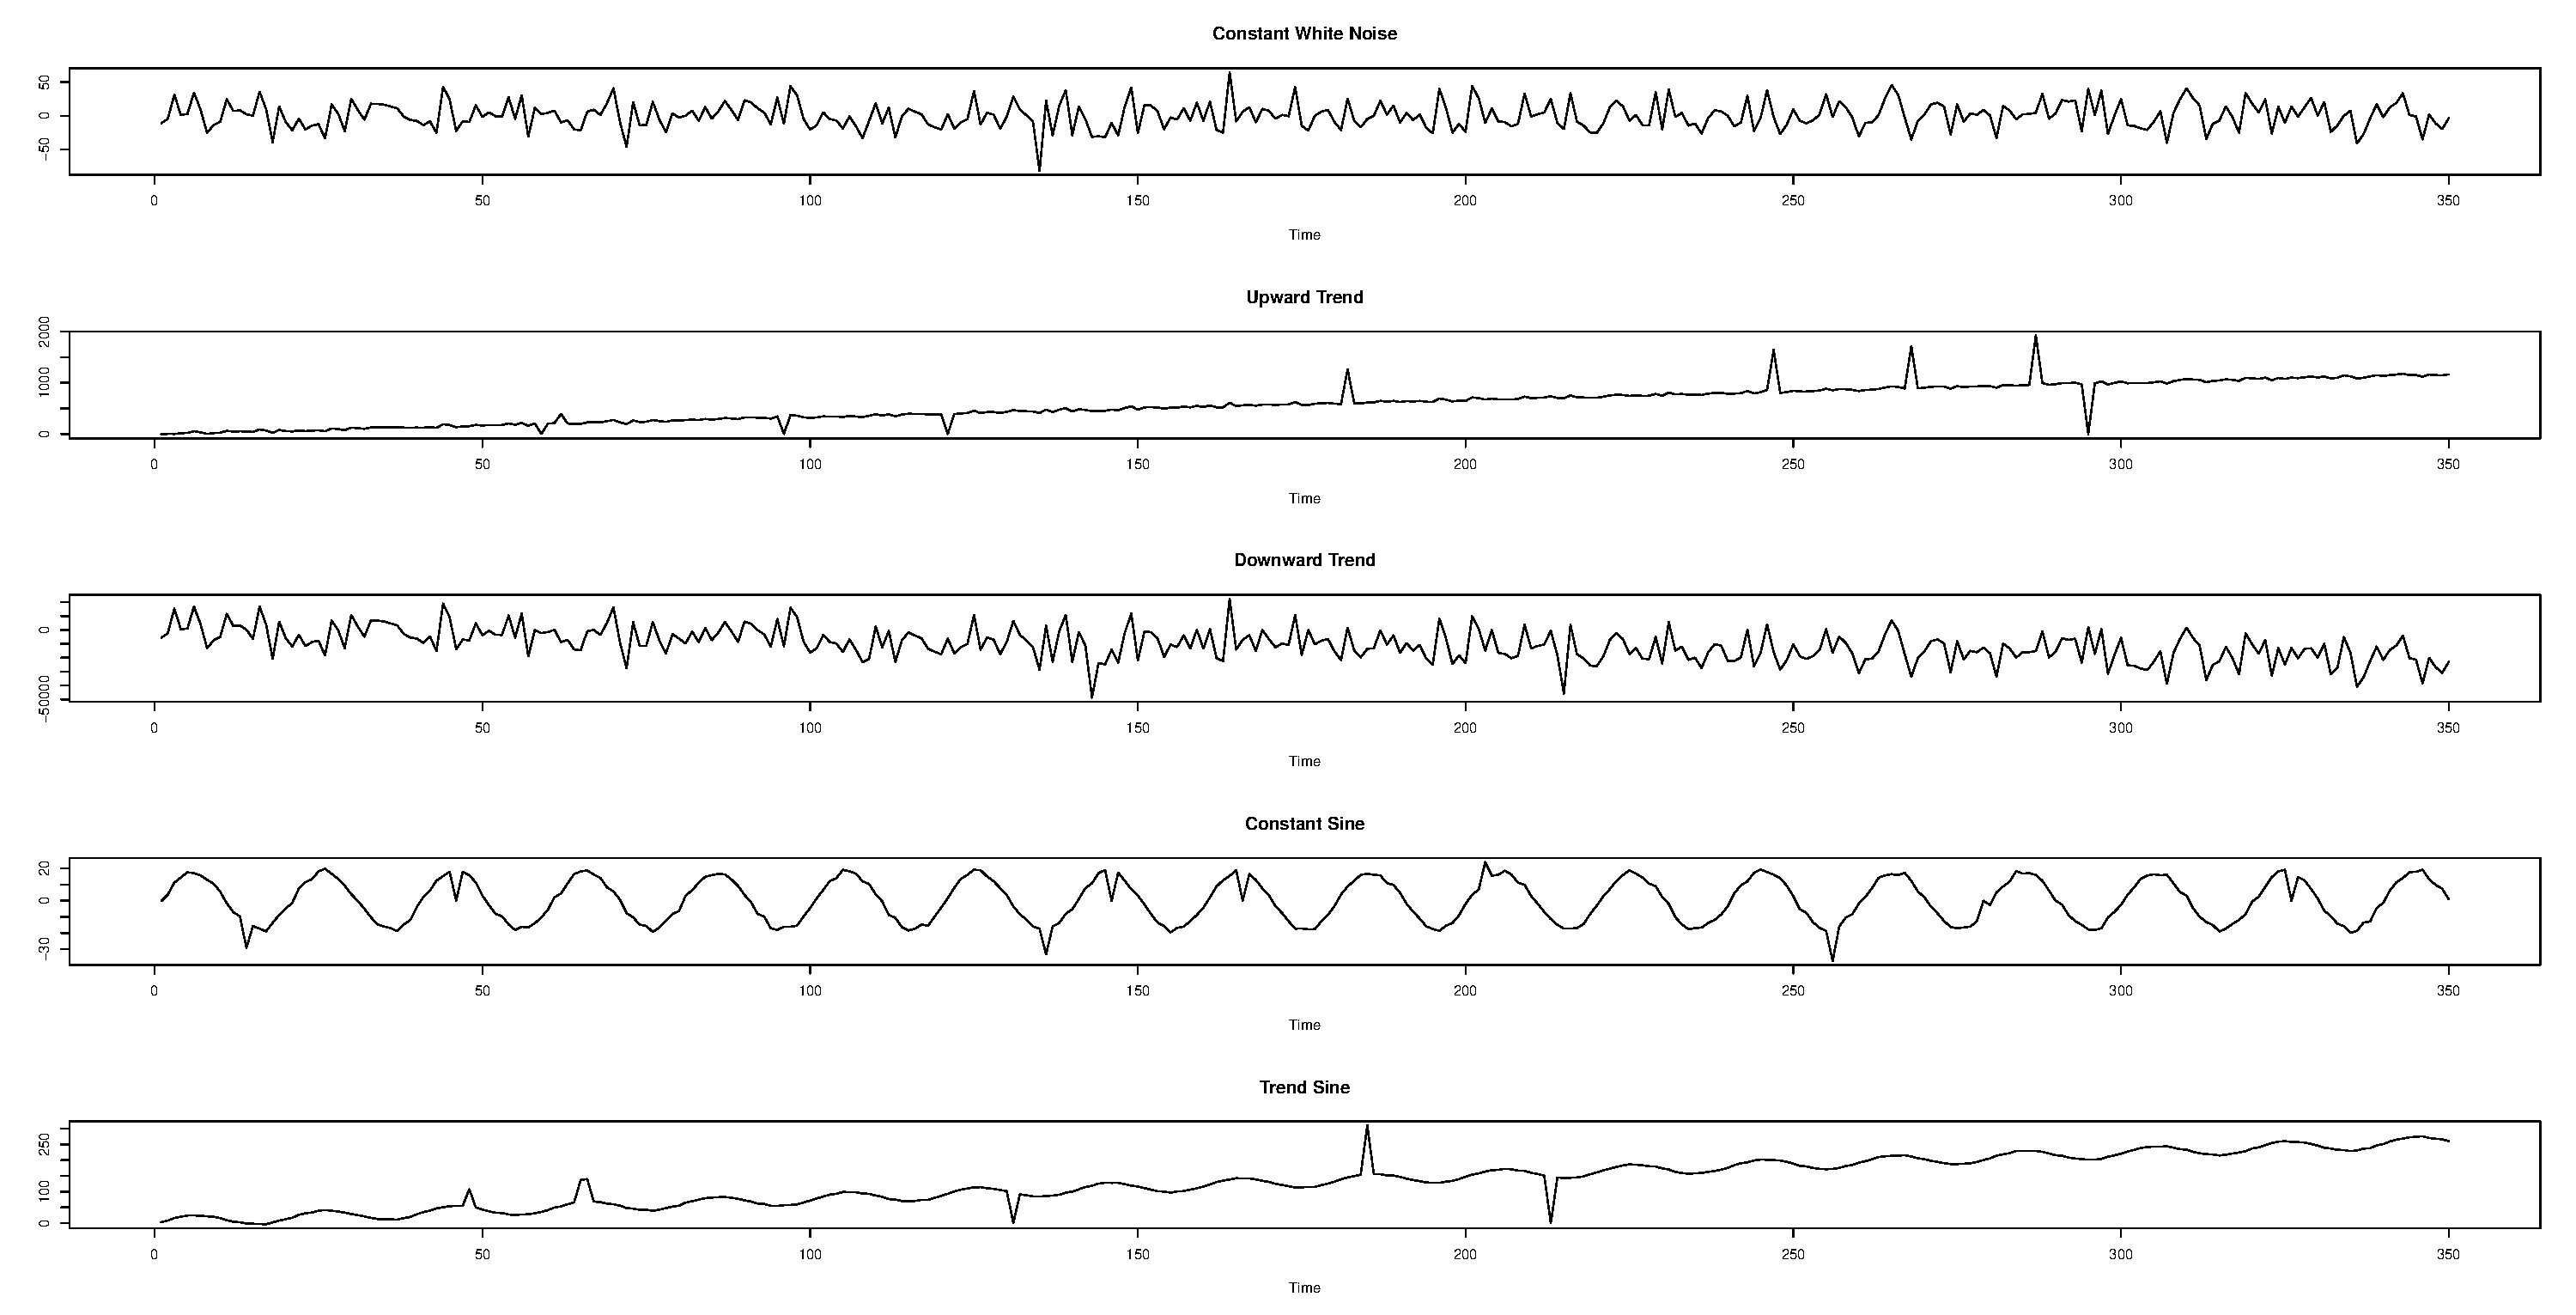
\includegraphics[angle=0]{img/testing-time-series.pdf}}
            \caption{Time series samples for evaluation.}
            \label{appen:img-testing-samples}
        \end{center}
    \end{figure}

\chapter{Tests Results} \label{appen:chap:results}

    \begin{table}[h]
        \begin{center}
            \begin{tabular}{c|c|c|c|c|c}
                \textbf{Test case} &
                \rotatebox{90}{wn} &  \rotatebox{90}{\texttt{trendUpLow}} & \rotatebox{90}{\texttt{trendDownHigh}} &
                \rotatebox{90}{\texttt{sine}} & \rotatebox{90}{\texttt{sineTrend}} \\ \hline \hline
                \multirow{2}{*}{48\,--\,12 (1)}   & 252.60 & 4293.10 & 59074630.35 & 19.91 & 291.89 \\
                                                  & 251.72 & 4602.83 & 57931198.55 & 19.97 & 291.90 \\ \hline
                \multirow{2}{*}{100\,--\,12 (1)}  & 247.72 & 702.52  & 117983966.67 & 23.54 & 25.82 \\
                                                  & 252.96 & 513.46 & 124329179.62 & 23.54 & 26.30 \\ \hline
                \multirow{2}{*}{200\,--\,12 (1)}  & 380.51 & 862.58 & 100868036.49 & 45.14 & 50.91 \\
                                                  & 380.57 & 718.39 & 101969913.50 & 45.14 & 47.95 \\ \hline \hline

                \multirow{2}{*}{48\,--\,12 (6)}   & 333.07 & 7071.66 & 90579713.93 & 483.70 & 1772.85\\
                                                  & 325.33 & 7206.03 & 89687108.81 & 483.88 & 1772.86 \\ \hline
                \multirow{2}{*}{100\,--\,12 (6)}  & 287.00 & 1916.31 & 125727085.38 & 420.33 & 346.06 \\
                                                  & 289.63 & 1531.48 & 130162180.73 & 420.33 & 347.18 \\ \hline
                \multirow{2}{*}{200\,--\,12 (6)}  & 325.67 & 1457.51 & 172882341.31 & 394.90 & 2734.56 \\
                                                  & 327.13 & 1132.87 & 172309610.96 & 394.90 & 2733.64 \\ \hline \hline

                \multirow{2}{*}{48\,--\,12 (12)}  & 271.78 & 7556.76 & 71166890.64 & 535.57 & 2956.52 \\
                                                  & 276.16 & 7742.00 & 71094737.26 & 535.46 & 2956.52 \\ \hline
                \multirow{2}{*}{100\,--\,12 (12)} & 239.68 & 12726.82 & 104525954.16 & 513.42 & 288.09 \\
                                                  & 251.44 & 12416.04 & 112937185.50 & 513.42 & 286.96 \\ \hline
                \multirow{2}{*}{200\,--\,12 (12)} & 381.57 & 2875.74 & 197649156.81 & 562.27 & 2064.04 \\
                                                  & 381.71 & 2316.18 & 196658315.76 & 562.27 & 2077.42 \\ \hline
            \end{tabular}
            \caption{Test results in MSE for simple exponential smoothing.}
            \label{appen:tab:simple-results}
        \end{center}
    \end{table}

    \begin{table}[h]
        \begin{center}
            \begin{tabular}{c|c|c|c|c|c}
                \textbf{Test case}  & \rotatebox{90}{wn} &
                \rotatebox{90}{\texttt{trendUpLow}} & \rotatebox{90}{\texttt{trendDownHigh}} &
                \rotatebox{90}{\texttt{sine}} & \rotatebox{90}{\texttt{sineTrend}} \\ \hline \hline
                \multirow{2}{*}{48\,--\,12 (1)}   & 272.33 & 3617.53 & 65694458.22 & 22.70 & 668.61 \\
                                                  & 279.60 & 3574.63 & 66644587.71 & 20.41 & 659.66 \\ \hline
                \multirow{2}{*}{100\,--\,12 (1)}  & 282.50 & 190.63 & 90967195.65 & 8.46 & 26.17 \\
                                                  & 302.91 & 193.77 & 93267732.29 & 9.40 & 25.61 \\ \hline
                \multirow{2}{*}{200\,--\,12 (1)}  & 399.27 & 361.50 & 108286781.11 & 35.56 & 48.96 \\
                                                  & 405.67 & 347.69 & 109496254.07 & 38.48 & 48.21 \\ \hline \hline

                \multirow{2}{*}{48\,--\,12 (6)}   & 354.67 & 6324.32 & 86541840.59 & 880.76 & 8031.60 \\
                                                  & 320.00 & 6454.35 & 77856708.99 & 856.96 & 7843.41 \\ \hline
                \multirow{2}{*}{100\,--\,12 (6)}  & 323.09 & 263.81 & 110815056.99 & 636.99 & 449.11 \\
                                                  & 332.08 & 253.23 & 100878861.50 & 673.94 & 420.09 \\ \hline
                \multirow{2}{*}{200\,--\,12 (6)}  & 324.50 & 316.76 & 167489984.23 & 811.24 & 2958.53 \\
                                                  & 340.14 & 374.38 & 162368879.38 & 830.81 & 2933.63 \\ \hline \hline

                \multirow{2}{*}{48\,--\,12 (12)}  & 275.92 & 3077.24 & 65058787.15 & 4394.80 & 29063.69 \\
                                                  & 299.00 & 3068.45 & 72999868.22 & 3921.33 & 28324.64 \\ \hline
                \multirow{2}{*}{100\,--\,12 (12)} & 272.97 & 13143.67 & 58829949.01 & 4919.03 & 565.68 \\
                                                  & 315.49 & 13449.97 & 76982996.39 & 4646.99 & 490.45 \\ \hline
                \multirow{2}{*}{200\,--\,12 (12)} & 376.87 & 423.64 & 186182717.66 & 5777.67 & 2507.91 \\
                                                  & 381.13 & 499.08 & 173511817.12 & 5462.19 & 2489.15 \\ \hline
            \end{tabular}
            \caption{Test results in MSE for double exponential smoothing.}
            \label{appen:tab:double-results}
        \end{center}
    \end{table}

    \begin{table}[h]
        \begin{center}
            \begin{tabular}{c|c|c}
                \textbf{Test case} &
                \rotatebox{90}{\texttt{sine}} & \rotatebox{90}{\texttt{sineTrend}} \\ \hline \hline
                \multirow{2}{*}{48\,--\,12 (1)}   & 11.24 & 25.08 \\
                                                  & 8.07 & 20.15 \\ \hline
                \multirow{2}{*}{100\,--\,12 (1)}  & 2.29 & 43.64   \\
                                                  & 2.09 & 57.07 \\ \hline
                \multirow{2}{*}{200\,--\,12 (1)}  & 15.92 & 88.18 \\
                                                  & 15.74 & 73.84 \\ \hline \hline

                \multirow{2}{*}{48\,--\,12 (6)}   & 9.26 & 390.64 \\
                                                  & 4.07 & 693.93 \\ \hline
                \multirow{2}{*}{100\,--\,12 (6)}  & 3.09 & 34.05 \\
                                                  & 2.44 & 37.11 \\ \hline
                \multirow{2}{*}{200\,--\,12 (6)}  & 4.19 & 1853.59 \\
                                                  & 5.65 & 1908.62 \\ \hline \hline

                \multirow{2}{*}{48\,--\,12 (12)}  & 4.31 & 965.75 \\
                                                  & 4.07 & 693.93 \\ \hline
                \multirow{2}{*}{100\,--\,12 (12)} & 2.26 & 8.44 \\
                                                  & 2.15 & 7.48 \\ \hline
                \multirow{2}{*}{200\,--\,12 (12)} & 0.95 & 1954.75 \\
                                                  & 2.63 & 1924.38 \\ \hline
            \end{tabular}
            \caption{Test results in MSE for triple exponential smoothing.}
            \label{appen:tab:triple-results}
        \end{center}
    \end{table}

\chapter{Source Code Metrics}
    \paragraph*{Number of Java files:} 105
    \paragraph*{Number of lines:} 9782
    \paragraph*{Size of the WAR archive of \texttt{hawkular-dataminig-dist} module} : 8744B

\chapter{Content of the Attachment}
    \paragraph*{Directory \texttt{doc}:} \LaTeX source code of this thesis.
    \paragraph*{Directory \texttt{src}:} source code of Data Mining module.
    \paragraph*{Directory \texttt{src-hawkular}:} source code of Hawkular with integrated Data Mining.
    \paragraph*{Directory \texttt{bin}:} binaries of Data Mining and Hawkular with integrated Data Mining.

\end{document}
